% **************************************************************************************************************
% A Classic Thesis Style
% An Homage to The Elements of Typographic Style
%
% Copyright (C) 2010 Andr� Miede http://www.miede.de
%
% If you like the style then I would appreciate a postcard. My address 
% can be found in the file ClassicThesis.pdf. A collection of the 
% postcards I received so far is available online at 
% http://postcards.miede.de
%
% License:
% This program is free software; you can redistribute it and/or modify
% it under the terms of the GNU General Public License as published by
% the Free Software Foundation; either version 2 of the License, or
% (at your option) any later version.
%
% This program is distributed in the hope that it will be useful,
% but WITHOUT ANY WARRANTY; without even the implied warranty of
% MERCHANTABILITY or FITNESS FOR A PARTICULAR PURPOSE.  See the
% GNU General Public License for more details.
%
% You should have received a copy of the GNU General Public License
% along with this program; see the file COPYING.  If not, write to
% the Free Software Foundation, Inc., 59 Temple Place - Suite 330,
% Boston, MA 02111-1307, USA.
%
% **************************************************************************************************************
% Note:
%    * You must not use "u etc. in strings/commands that will be spaced out (use \"u or real umlauts instead)
%    * New enumeration (small caps): \begin{aenumerate} \end{aenumerate}
%    * For margin notes: \graffito{}
%    * Do not use bold fonts in this style, it is designed around them
%    * Use tables as in the examples
%    * See classicthesis-ldpkg.sty for useful commands
% **************************************************************************************************************
% To Do:
%    * [high] Check this out: http://www.golatex.de/koma-script-warnung-in-verbindung-mit-listings-package-t2058.html
%    * [medium] mathbb in section-titles/chapter-titles => disappears somehow in headlines!!!
%    * [low] Calculate text block size for Libertine font
%    * [low] Think about processing a4paper, a5paper, 10pt, 11pt, 12pt etc. options for typearea layout
%            (store values in internal variables and handle by \AtEndOfPackage{\areaset...})
% **************************************************************************************************************
\documentclass[ twoside,openright,titlepage,fleqn,numbers=noenddot,headinclude,%1headlines,footinclude
                11pt,letterpaper,BCOR5mm,cleardoublepage=empty,abstractoff % <--- obsolete, remove (todo)
                ]{scrreprt}
% ********************************************************************
% Development Stuff
% ********************************************************************
\listfiles
%\usepackage[l2tabu, orthodox, abort]{nag}
%\usepackage[warning, all]{onlyamsmath}
% ********************************************************************
% Re-usable information
% ********************************************************************
\newcommand{\myTitle}{A Substrate for Accountable Layered Systems\xspace}
\newcommand{\myDegree}{Ph.D. in the Media Arts and Sciences\xspace}
\newcommand{\myName}{Bo Morgan\xspace}
\newcommand{\myProf}{Marvin Minsky\xspace}
\newcommand{\myOtherProf}{Gerald Sussman\xspace}
\newcommand{\mySupervisor}{Joseph Paradiso\xspace}
\newcommand{\myFaculty}{Put data here\xspace}
\newcommand{\myDepartment}{Media Lab\xspace}
\newcommand{\myUni}{\protect{Massachusetts Institute of Technology}\xspace}
\newcommand{\myLocation}{Cambridge\xspace}
\newcommand{\myTime}{September 2012\xspace}
\newcommand{\myVersion}{Version 1.0\xspace}
%*******************************************************
% Packages with options that might require adjustments
%*******************************************************
\usepackage[latin1]{inputenc}
\usepackage[ngerman,american]{babel}
\usepackage{natbib}
%\usepackage[square,numbers]{natbib}
\usepackage[fleqn]{amsmath} % math environments and more by the AMS

%*******************************************************
\usepackage{classicthesis-ldpkg} % [backref]
%*******************************************************
% Options for classicthesis.sty:
% tocaligned eulerchapternumbers drafting linedheaders listsseparated 
% subfig nochapters beramono eulermath parts minionpro pdfspacing 
% listings dottedtoc minionprospacing manychapters
\usepackage[eulerchapternumbers,drafting,listings,listsseparated,%pdfspacing,%listings,
            subfig,beramono,eulermath,parts,manychapters]{classicthesis}

%*******************************************************
% Some font experiments
%*******************************************************
%\usepackage[osf]{libertine}
%\usepackage{hfoldsty}
%\usepackage[light,condensed,math]{iwona}
%\renewcommand{\sfdefault}{iwona}
%\usepackage{lmodern} % <-- no osf support :-(
%\usepackage[urw-garamond]{mathdesign} <-- no osf support :-(

%*******************************************************
% Fine-tuning for the text area
%*******************************************************
%\linespread{1.05} % a bit more for Palatino
%\areaset[5mm]{312pt}{761pt} % 686 (factor 2.2) + 33 head + 42 head \the\footskip
%\setlength{\marginparwidth}{7em}%
%\setlength{\marginparsep}{2em}%

%*******************************************************
% hack to use citations in float environments 
% will be fixed with caption package version 3.2
%*******************************************************
\usepackage{makerobust} 
\makeatletter 
%\MakeRobustCommand\caption@xref 
\makeatother 




\usepackage{amsthm} % defines \newtheorem
\newtheorem{expression}{Expression}[section] % Funk2 expression
\newtheorem{definition}{Definition}[chapter] % mathematical definition

% BEGIN DRAFT WATERMARK CODE
%
% This code is from
% http://filoxus.blogspot.com/2008_01_01_archive.html
%
% Thanks to the ``Daily rant: A random blog about everything, mostly
% programming''

\usepackage{graphicx}
\usepackage{type1cm}
\usepackage{eso-pic}
\usepackage{color}

\makeatletter
\AddToShipoutPicture{
  \setlength{\@tempdimb}{.5\paperwidth}
  \setlength{\@tempdimc}{.5\paperheight}
  \setlength{\unitlength}{1pt}
  \put(\strip@pt\@tempdimb,\strip@pt\@tempdimc){
%    \makebox(0,0){
%      \rotatebox{45}{
%        \makebox(-72,0){
%          \vspace{3cm}\textcolor[gray]{0.875}{{\fontsize{3cm}{3cm}\selectfont{UNOFFICIAL}}}
%        }
%      }
%    }
%    \makebox(0,0){
%      \rotatebox{45}{
%        \makebox(-72,0){
%          \vspace{-6cm}\textcolor[gray]{0.875}{{\fontsize{6cm}{6cm}\selectfont{DRAFT}}}
%        }
%      }
%    }
    \makebox(0,0){
      \rotatebox{45}{
        \vspace{-6cm}\textcolor[gray]{0.9375}{{\fontsize{6cm}{6cm}\selectfont{DRAFT}}}
      }
    }
  }
}
\makeatother

% END DRAFT WATERMARK CODE


%*******************************************************            
%\usepackage[section,below]{placeins} <--- not everybody wants this
%\usepackage[all]{hypcap} <--- does not work with MiKTeX 2.6
% ********************************************************************
% Language/strings for backrefs (change here, thanks, Lorenzo)
%*******************************************************
%\renewcommand{\backrefnotcitedstring}{\relax}%(Not cited.)
%\renewcommand{\backrefcitedsinglestring}[1]{(Citato a pagina~#1.)}
%\renewcommand{\backrefcitedmultistring}[1]{(Citato alle pagine~#1.)}
%\renewcommand{\backreftwosep}{ e~}
%\renewcommand{\backreflastsep}{ e~}
% ********************************************************************
% Setup and Finetuning
%*******************************************************
\newlength{\abcd} % for ab..z string length calculation
\newcommand{\myfloatalign}{\centering} % how all the floats will be aligned
\setlength{\extrarowheight}{3pt} % increase table row height
% ********************************************************************
% Captions look and feel
%*******************************************************
\captionsetup{format=hang,font=small}
% ********************************************************************
% Listings setup
% ********************************************************************
%\lstset{emph={trueIndex,root},emphstyle=\color{BlueViolet}}%\underbar} % for special keywords
% ********************************************************************
\lstset{language=[LaTeX]Tex,%C++,
    keywordstyle=\color{RoyalBlue},%\bfseries,
    basicstyle=\small\ttfamily,
    %identifierstyle=\color{NavyBlue},
    commentstyle=\color{Green}\ttfamily,
    stringstyle=\rmfamily,
    numbers=none,%left,%
    numberstyle=\scriptsize,%\tiny
    stepnumber=5,
    numbersep=8pt,
    showstringspaces=false,
    breaklines=true,
    frameround=ftff,
    frame=single,
    belowcaptionskip=.75\baselineskip,
    %numberbychapter=false
    %frame=L
}

% ********************************************************************
% Where to look for graphics
%*******************************************************
%\graphicspath{{gfx/}{misc/}} % considered harmful according to l2tabu
% ********************************************************************
% Hyperreferences
%*******************************************************
\hypersetup{%
    colorlinks=true, linktocpage=true, pdfstartpage=3, pdfstartview=FitV,%
    % uncomment the following line if you want to have black links (e.g., for printing)
    %colorlinks=false, linktocpage=false, pdfborder={0 0 0}, pdfstartpage=3, pdfstartview=FitV,% 
    breaklinks=true, pdfpagemode=UseNone, pageanchor=true, pdfpagemode=UseOutlines,%
    plainpages=false, bookmarksnumbered, bookmarksopen=true, bookmarksopenlevel=0,%
    hypertexnames=true, pdfhighlight=/O,%hyperfootnotes=true,%nesting=true,%frenchlinks,%
    urlcolor=webbrown, linkcolor=RoyalBlue, citecolor=webgreen, %pagecolor=RoyalBlue,%
    %urlcolor=Black, linkcolor=Black, citecolor=Black, %pagecolor=Black,%
    pdftitle={\myTitle},%
    pdfauthor={\textcopyright\ \myName, \myUni, \myFaculty},%
    pdfsubject={},%
    pdfkeywords={},%
    pdfcreator={pdfLaTeX},%
    pdfproducer={LaTeX, HyperRef, ClassicThesis, GraphViz, and LibreDraw}%
}




\usepackage{rotating}



% BEGIN LONG DIVISION DIGIT SPACING
%
\newdimen\digitwidth
\settowidth\digitwidth{0}
\def~{\hspace{\digitwidth}}

\def\longdivisionrule#1#2{%
\noalign{\moveright#1\digitwidth%
\vbox{\hrule width#2\digitwidth}}}

%101\,\begin{tabular}[b]{@{}r@{}}
%10010 \\ \hline
%\big)\begin{tabular}[t]{@{}l@{}}
%1011110 \\
%101 \\ \longdivisionrule{0}{7}
%~~~111 \\
%~~~101 \\ \longdivisionrule{3}{4}
%~~~~100
%\end{tabular}
%\end{tabular}
%
% END LONG DIVISION DIGIT SPACING


% BEGIN EQUATION SECTION NUMBERING
%
%\numberwithin{equation}{section}
%
% END EQUATION SECTION NUMBERING








%********************************************************************
% Hyphenation
%*******************************************************
%\hyphenation{put special hyphenation here}
% ********************************************************************
% GO!GO!GO! MOVE IT!
%*******************************************************
\begin{document}
\frenchspacing
\raggedbottom
\selectlanguage{american} % american ngerman
%\renewcommand*{\bibname}{new name}
%\setbibpreamble{}

%% remarked for starting pages with 1
%\pagenumbering{roman}

\pagestyle{plain}
%********************************************************************
% Frontmatter
%*******************************************************
%*******************************************************
% Little Dirty Titlepage
%*******************************************************
\thispagestyle{empty}
%\pdfbookmark[1]{Titel}{title}
%*******************************************************
\begin{center}
    \spacedlowsmallcaps{\myName} \\ \medskip                        

    \begingroup
        \color{Maroon}\spacedallcaps{\myTitle}
    \endgroup
\end{center}        

{\flushright{Advisor\hspace{0.5cm}          \makebox[3in]{\hrulefill}}}

{\flushright{Committee Member\hspace{0.5cm} \makebox[3in]{\hrulefill}}}


%*******************************************************
% Titlepage
%*******************************************************
\begin{titlepage}
  % if you want the titlepage to be centered, uncomment and fine-tune the line below (KOMA classes environment)
  \begin{addmargin}[-1cm]{-3cm}
    \begin{center}
      \large  
      
      \hfill
      
      \vfill
      
      \begingroup
      \color{Maroon}\spacedallcaps{\myTitle} \\ \bigskip
      \endgroup
      
      \spacedlowsmallcaps{\myName}
      
      \vfill
      
      \includegraphics[height=7cm]{gfx/model-6} \\ \medskip
      
      \vspace{5mm}

      \myDegree \\ \medskip
      \myDepartment \\                            
      %\myFaculty \\
      \myUni \\ \bigskip
      
      \myTime
      
      \vfill                      
      
    \end{center}  
  \end{addmargin}       
\end{titlepage}   

\include{frontbackmatter/titleback}
\cleardoublepage%*******************************************************
% Dedication
%*******************************************************
\thispagestyle{empty}
%\phantomsection 
\refstepcounter{dummy}
\pdfbookmark[1]{Dedication}{Dedication}

\vspace*{3cm}

\begin{center}
    Don't do anything that isn't play. \\ \medskip
    --- Joseph Campbell
\end{center}

\medskip

\begin{center}
    Dedicated to the loving memory of Push Singh. \\ \smallskip
    1972\,--\,2006
\end{center}

\cleardoublepage%*******************************************************
% Abstract
%*******************************************************
%\renewcommand{\abstractname}{Abstract}
\pdfbookmark[1]{Abstract}{Abstract}
\begingroup
\let\clearpage\relax
\let\cleardoublepage\relax
\let\cleardoublepage\relax

\chapter*{Abstract}
%Between the ages of 1-3 years old, children display primary emotions,
%such as joy, disappointment, and surprise.  These emotional processes
%have been hypothesized to be related to the process of failing or
%succeeding to accomplish a goal.  Around age 4, children begin to
%display emotions that involve the self, such as guilt and shame.  It
%has been hypothesized that these emotions relate to another person's
%evaluation of the child's goals as good or bad.
%
%We approach modelling this developmental process by applying Marvin
%Minsky's theory of the child-imprimer relationship.  According to
%Minsky's theory, at a young age, a human child becomes attached to a
%person that functions as a teacher.  The imprimer could be a parent or
%a caregiver or another person in the child's life, but the function of
%the imprimer is to provide feedback to the child in terms of what
%goals are good or bad for the child to pursue.




Recently, there have been two directions of research with the goal of
building a machine that explains intelligent human behavior.  The
first approach is the machine learning approach and the second is the
pattern recognition approach.  Each of these solutions has benefits
and drawbacks.  The machine learning approach attempts to build a
machine that learns to accomplish goals by learning the effects of its
actions by interacting with its environment.  The pattern recognition
approach is given large amounts of knowledge and finds statistical
regularities within this knowledge in order to generate more
knowledge.  Machine learning is good for dealing with novel problems,
but these problems are necessarily simple because complex problems
require background knowledge.  Pattern recognition deals well with
complicated problems requiring a lot of background knowledge, but
fails to adapt to changing environments, for which the algorithm has
not already been trained.

We are working on an algorithm that combines these two extremes into
an algorithm that inherits cultural language knowledge, while
recognizing the failures of this knowledge through failures and
successes when this knowledge is used.  We develop a definition of the
utility of cultural knowledge in a domain that is grounded in
goal-oriented action that corrects this knowledge by learning in the
context of failure and success.





\endgroup

\vfill

\cleardoublepage%*******************************************************
% Publications
%*******************************************************
\pdfbookmark[1]{Publications}{publications}
\chapter*{Publications}
Some ideas and figures have appeared previously in the following publications:

\bigskip

\noindent Morgan, B.; ``Moral Compass: Commonsense Social Reasoning
 Cognitive Architecture''; http://em-two.net/about; Commonsense Tech
 Note; MIT Media Lab; 2011 January

\vspace{5mm}

\noindent Smith, D. and Morgan, B.; "IsisWorld: An open source
 commonsense simulator for AI researchers"; AAAI 2010 Workshop on
 Metacognition; 2010 April

\vspace{5mm}

\noindent Morgan, B.; ``A Computational Theory of the Communication of
 Problem Solving Knowledge between Parents and Children''; PhD
 Proposal; MIT Media Lab 2010 January

\vspace{5mm}

\noindent Morgan, B.; ``Funk2: A Distributed Processing Language for 
 Reflective Tracing of a Large Critic-Selector Cognitive
 Architecture''; Proceedings of the Metacognition Workshop at the
 Third IEEE International Conference on Self-Adaptive and
 Self-Organizing Systems; San Francisco, California, USA; 2009
 September

\vspace{5mm}

\noindent Morgan, B.; ``Learning Commonsense Human-language Descriptions
 from Temporal and Spatial Sensor-network Data''; Masters Thesis;
 Massachusetts Institute of Technology; 2006 August

\vspace{5mm}

\noindent Morgan, B.; ``Learning perception lattices to compare
 generative explanations of human-language stories''; Published
 Online; Commonsense Tech Note; MIT Media Lab; 2006 July

\vspace{5mm}

\noindent Morgan, B. and Singh, P.; ``Elaborating Sensor Data using
 Temporal and Spatial Commonsense Reasoning''; International Workshop
 on Wearable and Implantable Body Sensor Networks (BSN-2006); 2005
 November

\vspace{5mm}

\noindent Morgan, B.; ``Experts think together to solve hard problems'';
 Published Online; Commonsense Tech Note; MIT Media Lab 2005 August

\vspace{5mm}

\noindent Morgan, B.; ``LifeNet Belief Propagation''; Published Online;
 Commonsense Tech Note; MIT Media Lab; 2004 January

\cleardoublepage%*******************************************************
% Acknowledgments
%*******************************************************
\pdfbookmark[1]{Acknowledgments}{acknowledgments}

%Don't do anything that isn't play. \\ \medskip
%    --- Joseph Campbell



\begin{flushright}{\slshape    
Don't do anything that isn't play.} \\ \medskip
    --- Joseph Campbell
\end{flushright}



\bigskip

\begingroup
\let\clearpage\relax
\let\cleardoublepage\relax
\let\cleardoublepage\relax
\chapter*{Acknowledgments}

I would first like to thank:

\begin{itemize}
\item{Push Singh for being an inspiring friend and advisor.}
\end{itemize}

Next, I would like to thank my committee:

\begin{itemize}
\item{Joe Paradiso for unfailing support and faith in my ability to do
  something well.}
\item{Marvin Minsky for consistently and patiently providing an
  inspiringly critical perspective and a wealth of important problems
  to solve.}
\item{Gerry Sussman for loving to program.}
\item{Mike Cox for providing critical direction for navigating the
  space of the contemporary meta-cognitive computational sciences.}
\end{itemize}

I would next like to thank my immediate family:

\begin{itemize}
\item{Greg Morgan and Carolyn Spinner for being supportive parents---willing to help me think about anything at any time.}
\item{Paul Bergman for teaching me how to program.}
\item{Virginia Barasch for painting my finger nails.}
\item{Leaf Morgan for playing Archon with me.}
\end{itemize}

Professors and Scientists: Walter Bender, Henry Lieberman, Whitman
Richards, Ed Boyden, Sebastian Seung, Hugh Herr, Ted Selker, Rebecca
Saxe.

Popes: Dustin Smith, Scotty Vercoe, Dane Scalise.

Friends: Mako Hill, Barbara Barry.

\endgroup


\pagestyle{scrheadings}
\cleardoublepage\include{frontbackmatter/contents}
%\cleardoublepage%\manualmark
%\markboth{\spacedlowsmallcaps{Preface}}{\spacedlowsmallcaps{Preface}} % work-around to have small caps also
\refstepcounter{dummy}

%************************************************
\addtocontents{toc}{\protect\vspace{\beforebibskip}} % to have the bib a bit from the rest in the toc
\addcontentsline{toc}{chapter}{\tocEntry{Preface}}
%************************************************

\chapter*{Preface}
\chaptermark{Preface}


%*******************************************************
% Mainmatter
%*******************************************************

%% remarked for starting pages with 1
%\pagenumbering{arabic}

%************************************************
\chapter{Introduction}
\label{chapter:introduction}
%************************************************

In this dissertation I present the substrate for accountable layered
systems.  I have focused on building this substrate for doing
reflective thinking on a large scale in learning systems, using
{\mbox{\citeauthor{singh:2005b}'s~\citeyearpar{singh:2005b}}} example
of reflective architectures as the precedent.  My approach focuses on
a purely procedural approach that does not assume any logical search
algorithms that work behind-the-scenes without a reflective learning
focus.  Without increasing the computational time complexity of basic
search, this approach learns to search in $n$ concurrent layers of
goal-oriented optimization, learning to plan physical actions, while
concurrently learning to plan planning actions.  Physical activities
are presented as analogous to thinking activities, allowing a
recursive application of the model to itself.  The contributions of
this thesis are:

\begin{itemize}
\item \emph{Emotion Machine Cognitive Architecture}: A computational
  implementation of metacognition that contains a physical simulation
  that is controlled by a deliberative physical object-level reasoning
  layer with another reflective meta-level reasoning layer that learns
  to control the first-order problem solving resources.  This is the
  result of stacking two very similar planning machines on top of one
  another, pointing toward future reflective architectures that will
  be able to recursively ``grow'' layers of reflective planning over
  any given preexisting problem solving resources.
\item \emph{Grounded Learning of Knowledge Utility}: A dependency
  tracing learning algorithm that is capable of learning both from
  ``being told'' as well as from experience, learning what types of
  knowledge are useful in different contexts, correcting knowledge
  when it turns out to be wrong, learning and correcting assumptions
  of the utility of knowledge through experience acting in the
  physical world.
\item \emph{The Substrate for Accountable Layered Systems}: A
  concurrent and parallel lisp-like virtual machine and programming
  language with procedural tracing features that facilitate the
  automatic monitoring of control systems running many concurrent
  tasks.
\end{itemize}

\section{Closed-loop Control and Learning}

There are many artificial intelligence algorithms that provide
explanations for how to accomplish goals or gather rewards in a
domain. A basic artificial intelligence system consists of three
processes: (1) perceptual data are generalized and categorized to
learn induced abstract models, (2) abstract models are used to infer
expected hypothetical states, i.e. states of future, past, or
otherwise ``hidden'' variables, (3) actions are chosen based on
considerations of different action-dependent inferences.  While there
are many types of machine learning algorithms that focus on this
abstract 3-step closed-loop process of learning to control, the field
of metacognition \cite[]{cox_and_raja:2008} focuses on making at least
two layers of closed-loop systems. The first closed-loop learning
algorithm learns how to deal with the external world, while the second
closed-loop learning algorithm perceives the state of the algorithm
below. I see metacognition as a layering of learning algorithms, such
that the second layer algorithm learns from perceiving the activity of
the first layer and controls or modifies this first layer. While it
may be clear how to trace changes in the perceptual inputs of layer
one of the algorithm, it is less than clear how the second layer
learner should monitor the changes in the state of the first layer
learner.

\section{A Review of the Emotion Machine v1.0}

One system that implements commonsense reasoning, based on Minsky's
Emotion Machine theory of mind \cite[]{minsky:2006}, is a
metareasoning system for correcting faulty plans, called EM1 (Emotion
Machine, v1) \cite[]{singh:2005b}. EM1 is written in Lisp, using a
Prolog extension as the logical resolution tool. EM1 is a layered
architecture consisting of reactive, deliberative, and reflective
layers. Mental critics are represented as commonsense narratives that
result in queries to a collection of different Prolog knowledge
bases. The commonsense narratives are given to the system in a Lisp
format that is compiled into the knowledge bases as collections of
horn clauses. These knowledge bases consist of collections of
domain-specific horn clauses that are divided into physical, social,
and mental domains of reasoning. On top of this Prolog logical
substrate, the Lisp program is organized into layers as a
critic-selector model of mind. The narrative plans that are generated
by the deliberative layer are executed by a lower-layer, called the
reactive layer. Part of the reactive layer of the algorithm is written
in C and runs PID control loops in a simulated social two-wheeled
inverted pendulum type robot. EM1 demonstrates how a system can use
commonsense narratives in order to reason by analogy in order to
generate plans. Also, EM1 demonstrates a learning process that is
driven by reflective critical recognition of failure. Because of the
complexity of the rigid-body physics in the world, sometimes even the
most carefully constructed plans fail. EM1 has a layer of reflective
critics that debug deliberative narratives as they are being
interpreted by using a collection of commonsense narrative debugging
critics.  Using narratives about social situations, EM1 infers the
goals of the other agents in the world given partial knowledge of
their visible physical actions. When mistakes are made in this
inference process, the failure is recognized reflectively, after the
fact. Specific types of debugging responses are implemented for
different forms of critical failures. EM1 is a step toward a large and
complex commonsense reasoning agent with multiple layers of
metareasoning that inspect, control, and debug mental representations.

\section{The Simulation}

The second thesis contribution is an example of a mathematical
simulation model that gives answers for the following questions:
\begin{itemize}
\item How do we assign credit to the planning process and learn to
  plan?
\item When many individual processes interact in the solution of a
  common problem, for example, controlling a complicated parallel
  system, how is credit traced for decisions that have been made in
  performing actions?
\item How do we learn what particular knowledge is either good or bad
  at solving different types of problems?
\item How do we trace dependencies back to the point that models of
  planning can be learned?
\item How do algorithms currently assign credit backwards in time and
  how does this model relate to these methods?
\end{itemize}

In this thesis, I evaluate how well this model is able to learn, not
only at the ground level but also at the hypothesis manipulation
level, improving the ground learning performance.  This simulation
will be described as a potential path around the exponential search
explosion problem.  There is a certain ``curse of dimensionality,''
which limits a search algorithm from considering an exponentially
vanishing percentage of the possible search paths as the length of the
paths is increased.  The simulations are often defined in abstract
terms, such as logical relationships, in order to make abstract
simulations of large domains.  Large systems that have logical
relationships require search algorithms to evaluate the implications
of the declarative forms.  These systems fail because there is this
explosion of exponential search.  In my model, in analyzing the
simulation, the curse of dimensionality is reduced through layers of
planned heuristic learning.  Any given algorithm can be procedurally
traced, resulting in a stream of events that do not change the time
complexity of the original algorithm, while a reflective algorithm can
learn to optimize this original algorithm.  The details of the
simulation model are the basis of the computational substrate that
allows for this improvement.

\section{The Substrate}

The substrate is a system for developing large software applications,
which enables parallel and concurrent process control.  The advantage
is the system's ability to selectively pause these parallel processes
when bugs are encountered, so that they can be easily examined in this
paused state.  Additionally, there are intricate thread control
operations for these processes.  When they ``sleep'', they are removed
from the scheduler, allowing the substrate to focus computational
resources on other processes.  When required, thousands of sleeping
processes can efficiently be ``triggered'' awake.  The primary point
of the system is that while running many different problem solvers at
the same time, it has the ability to conveniently trace the
interactions between those problem solvers.  Thus, all of the memory
in this substrate allows for the tracing of all memory allocations and
mutations.  It is a frame-based system.  Many AI systems are
implemented in an object-oriented or frame-based representation.  This
allows for all of the commonly associated programming methodologies to
exist, e.g.  object types and inheritance.  The substrate includes a
high-level lisp-like programming language, so the compiler can be
redefined by the running program.  There are layered ``cognitive
architecture'' structural primitives included in the language.  This
allows the programmer to build a ``layer'' which contains ``agencies''
which contain ``resources''.  These resources then are able to exist
as ``minds'' which control ``physical worlds'' because these
primitives already exist in this substrate.  This substrate, which can
be downloaded as open-source software, serves as an extensible
platform for continuing research on this implementation of reflective
thinking.

\section{Document Overview}

{\mbox{\autoref{part:the_model}}} begins with a non-technical
description of the model of mind that is used as the basis of both the
mathematical simulation and the computational implementations.  In
{\mbox{\autoref{part:the_simulation}}}, I explain the modelling
assumptions that I make in transitioning to the mathematical notation
of the simulation model.  Using this notation, I explain how this
model can be used to reduce the complexity of search algorithms.  In
{\mbox{\autoref{part:the_implementation}}}, I give an explanation of
how this simulation is automated on a concurrent computer, the thesis
implementation, SALS, the substrate for accountable layered systems.
In conclusion, in {\mbox{\autoref{part:conclusion}}}, I discuss
promising directions for future research in not only AI but also the
other cognitive sciences.

The focus of the dissertation will be a description of the reflective
problem of learning-to-control.  I describe control in terms of layers
of reflective credit assignment because this simplifies understanding
the problem of learning-to-control.  The focus will be on the
implementation of credit assignment at the level of planning
activities and then describe an example of a computational simulations
of reflective learning in a block building physical domain.

\section{Programming}

An example problem domain called the block building domain is shown in
{\mbox{\autoref{figure:example_problem_domain}}}.  In this case, we
have two blocks, which have relationships with the objects in the
room, such as the table.  If the goal state is to get the physical
world to exist in a particular configuration, the stack of {\tt
  Block-2} on top of {\tt Block-1},
{\mbox{\autoref{figure:example_program}}} shows an example of a
program that a programmer might write to move this gripper around in
this block building domain.  In this program, the gripper has very
simple symbolic commands: {\tt move-right}, {\tt reach}, {\tt grab},
{\tt move-left}, {\tt drop}.  One can imagine that this program might
intend to pick up the green block and put it on the blue block.
\begin{figure}
\center
\includegraphics[width=10cm]{gfx/blocks_world_example-1}
\caption{An example problem domain.}
\label{figure:example_problem_domain}
\end{figure}
\begin{figure}
\center
\begin{tabular}{l}
\\
  {\tt ~~[defunk example-program []}~~ \\
  {\tt ~~~~[move-right]} ~~\\
  {\tt ~~~~[reach]} ~~\\
  {\tt ~~~~[grab]} ~~\\
  {\tt ~~~~[move-left]} ~~\\
  {\tt ~~~~[drop]]} ~~\\
\\
\end{tabular}
\caption{An example program.}
\label{figure:example_program}
\end{figure}

\section{State Space Planning}

State space planning can be thought of as automatic programming.
Planning refers to the computer's ability to write its own program.
In an algorithm that plans by using a search algorithm, there is an
initial state with a number of possible actions that may lead away
from this state.  We can move left; we can stop; we can move right.
We can imagine what the possible future states would be after each
action.  In an imagined future state, the gripper may be in a
different position.  An example of the exponential growth resulting
from continuing a planning search is shown in
{\mbox{\autoref{figure:combinatorial_explosion_example}}}.
\begin{figure}
\center
\includegraphics[width=10cm]{gfx/combinatorial_explosion_example}
\caption{Exponential growth in planning as search.}
\label{figure:combinatorial_explosion_example}
\end{figure}
If every considered state in a search has the same number of possible
actions, this search becomes an exponential search problem.  The
number of actions from each state is the \emph{branch factor} of the
search.  Exponential searches quickly become intractable, even in
state spaces with a reasonable number of actions.  For example, games
of chess are played to 20 levels deep with about 30 moves from each
state.  Thus, expanding this search tree gives $30^{20}$, or $3 \times
10^{29}$ plans.  If there were one billion computers that each
processed one billion plans per second in parallel, this search would
still take over ten thousand years to complete, and that is just to
play the first move!  The fastest algorithms include good heuristics,
e.g. a count of the number of pieces on the board for each player.

\section{Heuristics}

When a problem is exponential, it progresses for as long as can be
afforded computationally, traversing the state space, hopefully
finding the goal state in this large space of all possible
alternatives, but then stops, usually not able to find the required
answer to the problem in the given time or space limitations.
\emph{Heuristics} are one way to alleviate the problematic exponential
growth of the search tree.  In order to search more efficiently,
heuristics provide weightings over the search tree that give a metric
of distance to a completed plan.  Beam search is an example of a
heuristically weighted search that has a finite number of plans that
it considers, forgetting the rest.  As used in beam search, a
heuristic is a function that defines an ordering on search paths.  A
heuristic function defines whether or not a given plan will
successfully accomplish the goal, also, a heuristic gives a metric of
the planning time required until a plan is created that will
accomplish the goal.  The algorithm uses this information to guide the
search, thus reducing the branch factor of the search tree, reducing
the search problem.
{\mbox{\autoref{figure:combinatorial_explosion_example_with_heuristics}}}
shows the same exponential growth example with heuristic weightings
overlayed with blue arrows.
\begin{figure}
\center
\includegraphics[width=10cm]{gfx/combinatorial_explosion_example_with_heuristics}
\caption{Exponential growth example with heuristics.}
\label{figure:combinatorial_explosion_example_with_heuristics}
\end{figure}

\section{Representing Actions}

The planning as search problem assumes that we have a representation
of the world and a representation for the changes that actions
perform.  Given these models, the physical world can be simulated
according to different plans.  \cite{fikes:1972} describe an action
representation, called ``STRIPS'', that includes an object called a
\emph{transframe} for simulating actions.  In the STRIPS model, the
world is a set of symbols.  A transframe is composed of two sets: one
for the removals from the world and one for the additions to the
world.  A transframe represents a change between two states of the
world.  In a symbolic relational domain, the state space is a set of
symbolic relationships rather than just symbols.  Here is an example
of a symbolic relationship that could exist in a relational domain:
{\tt [block-1 is-on block-2]}.  Here is an example of a transframe for
the world in a relational domain: \emph{remove} {\tt [block-1 on
    table-1]} and \emph{add} {\tt [block-1 on block-2]}.  In
predicting the effects of an action on the world, STRIPS considers one
transframe for each action.  Transframes can also be dependent on the
current state of the world.  Although many function approximation
methods could be used, in my simulation model I have addressed the
problem of learning to predict the correct transframes in the terms of
{\mbox{\citeauthor{mitchell:1997}'s~\citeyearpar{mitchell:1997}}}
``hypothesis spaces,'' which provide a simple and understandable
formulation of the category hypothesis learning problem, given
labelled examples.  Hypothetical models are learned to predict the
effects of actions.  The physical state space informs sets of
hypotheses that can be used to support assumptions, thus, the creation
of new knowledge from an absence of knowledge, given the listed
assumptions.

\section{Learning to Plan for Successful Execution}

Dependency traces for a hypothesized successful plan creation compose
an important set of knowledge to associate with a plan for debugging
the planning process when, later, it is realized that the plan fails
to execute.  {\mbox{\autoref{figure:dependency_traces}}} shows a
picture of dependency traces with hypothesis creation events being
pictured as shapes on a time line.  These hypotheses have arrows
between them that represent the derivation dependencies of each
hypothesis creating decision.  The circles in the picture represent
the symbolic states of the world that are used to create hypotheses,
which are represented by squares.  If any hypothesis is used to derive
another hypothesis, these dependencies give a credit assignment path
that is able to jump back retrospectively an arbitrary distance in
time as well as between reflective layers.  Notice in the picture that
the circle on the far left is a dependency of a square block, but
these two events are not necessarily consecutive in time.  If a
hypothesis is derived from a number of other hypotheses, possibly far
in the past, and this hypothesis fails in action, each one of these
traced dependencies represents a learning opportunity.  Every
additional layer of reflective control in the model, represents
another hypothetical learning opportunity, leading to more efficient
search toward plans that succeed in execution.
\begin{figure}
\center
\includegraphics[width=10cm]{gfx/dependency_traces}
\caption[Dependency traces.]{Dependency traces, where circles are
  symbols, squares are hypotheses, and arrows are dependencies.}
\label{figure:dependency_traces}
\end{figure}

\section{Finding a Bug}

The credit assignment problem arises when a bug occurs in some part of
the system.  For example, plans can fail physically to accomplish what
they have been previously hypothesized to accomplish.  There are many
knowledge dependency algorithms that work at this physical knowledge
level.  In this thesis, a layered reflective knowledge representation
is presented for propagating failures to knowledge manipulation
actions as well as physical actions.
{\mbox{\autoref{figure:tracing_bug_dependencies}}} represents a bug
found in a planning hypothesis.  For example, the planning hypothesis
could be that some certain planning activity leads from one type of
plan to a plan that will successfully complete execution without
failing.  Failure propagates through reflective layers of goals and
distinct classes of hypotheses.  Bugs are propagated through every
reflective layer and, therefore, each reflective layer is presented
with a different learning opportunity.
\begin{figure}
\center
\includegraphics[width=10cm]{gfx/tracing_bug_dependencies}
\caption[Tracing bug dependencies.]{Tracing bug dependencies, where
  the bold arrows represent the credit assignment path for a failure
  in a hypothesis, represented by the red square on the far right.}
\label{figure:tracing_bug_dependencies}
\end{figure}

\section{Reflection}

The term reflection is a commonly used word in computer science and
AI.  The idea is extremely simple and is the focus of this thesis,
but, because of its simplicity, it is a widely applicable idea.  In
fact, \cite{maes:1988} distinguishes over 30 different types of
\emph{computational reflection}, grounded in the computer science
literature.  The type of computational reflection that is introduced
in this dissertation is not included in Maes' overview, although the
implementation of this model is based on many of the forms of
computational reflection that Maes does describe, e.g. procedural
reflection, type reflection, frame reflection, and others.  She does
not mention the type of reflection that I am focused on in this thesis
because it was not, at the time, commonly considered computational.
The type of reflection that is modelled here is a psychological type
of reflection: the ability to think about thinking in addition to the
ground problem.  This psychological form of reflection is the focus of
this thesis.

In terms of this model, reflection is the ability to perceive, act,
and plan mental activities.  A planning process is a type of mental
activity, weighing decisions, making plans, and trying to accomplish
goals.  A process that optimizes this planning activity by, for
example, learning heuristics for the planning search, is an example of
a reflective process.  In general, this layered reflective model
learns in reaction to bugs and relearns the planning processes through
dependency tracing for credit assignment.  This model is similar to
current models of \emph{metacognition}, which will be described as
related research.

\section{The Derivative Nature of the Contributions}

The three primary contributions of the thesis are: (1) the
implementation, (2) the simulation, and (3) the model of mind.  My
primary contribution is explained last because it is a derivative of
the first two.  The model of mind is the simplest contribution and
serves as a foundation for the other two.  The simulation model
introduces a discrete state space to the model of mind, so that a
mathematical description can be given of the model of mind.  The
implementation model introduces a computational definition of the
transfer function for the state space introduced in the simulation
model.  Each of these contributions builds on the simpler, prior
contribution.  Therefore, in order to explain the implementation, I
begin with the simplest contribution and work through each additional
component in order to accomplish the primary goal of explaining the
computational implementation of reflective thinking.
{\mbox{\autoref{figure:layers_of_contributions}}} shows the derivative
nature of the contributions of the thesis in the order that they will
be described from most foundational to most abstract.
\begin{figure}
\center
\begin{tabular}{p{3.5cm}p{6.5cm}}
The Model:          & A foundation for how to think about reflective thinking. \\
The Simulation:     & Introduces a discrete state space to the model for a mathematical description of reflective thinking. \\
The Implementation: & Introduces a computational transfer function to the model for automatically simulating the mathematical description of reflective thinking.
\end{tabular}
\caption{The derivative nature of the contributions.}
\label{figure:layers_of_contributions}
\end{figure}

%\section{Hypotheses and Decisions}

%let me just go through a simple example of what a decision is because this becomes very confusing very quickly if we don't ground that idea out.
%this dog looks hungry should i feed him?
%he may bite me.
%this is a basic decision, so let's say we have two options
%how do we think about modelling these two options.
%we're in a current state
%it could possibly lead to two other states
%the question is: what action should we take?
%there is a lot of complicated processing that could into making this decision, but if we just want to talk about the basic development of what a hypothesis is and how do we develop the provenance of data based on that.
%that's what i'm building this up to.
%we have to choose of all of the knowledge we have, maybe from the current state, maybe from the past, which should this decision be based on?
%that's a very complicated problem.
%generally these algorithms are focused on a dataset, so they're not required to learn those types of relationships.
%how should i weigh my relative goals into this decision?
%certain algorithms will have a clear ranking of goals, like a reinforcement learning algorithm will have basically, any time you get into an important state, it will give you an exact number, this state was worth this much.
%this state was worth ten.
%this state was worth negative ten.
%the system that i'm talking about is a little more general than that.
%it uses multiple goals.
%they can have partial orderings.
%but you have to consider, some of the may not even be directly related, so you may have to, part of this decision process could be coming up with that partial order.
%i'd like to dog to not be hungry.
%i also don't want to be bitten.
%you're defining the states of the world that you're going to pay attention to.
%what might be the results of this?
%what might be the relationships?
%what are the relationships now that might help us to make this decision?
%for example, the properties of the dog that we might be paying attention to.
%let's say, there is a hunger for the dog.
%he looks hungry or he looks full.
%these are all things that we're perceiving to make this decision.
%the dog has a color, a breed, it could be barking or not, its going to tell us whether or not the dog is going to bite us basically.
%how do we develop a hypothesis?
%we may have multiple sets of training data.
%this may be our first example.
%we want to take the current situation and we want to make a prediction.
%what kind of hypotheses could we use?
%what does a hypothesis even look like?
%if we feed the dog, there are a bunch of things that might happen.
%he could fall asleep.
%he could continue to be hungry.
%here's a set of examples.
%imagine that we're feeding these examples into the algorithm 1 through 4 on the lefthand side there.
%there are a number of properties that we could then categorize into, for each of these numbered examples we could predict the category on the right.
%we're trying to predict whether or not our hand was bitten given the features on the dog.
%it's basically a function approximation algorithm that we're trying to develop as a hypothesis for this state space.
%
%minsky: mark twain had advice about buying a stock.
%if it goes up sell it.
%if it goes down don't but it.
%
%bo: i think there's a loop in that causal chain.
%i've tried to avoid those.
%
%what's the point?
%why are we talking about this?
%goals!
%because we have goals.
%there are good parts of the world
%there are bad parts of the world
%we want to know how to get to the good parts and avoid the bad parts
%we have avoidances
%we have goals
%we have states of the world
%these might be partial states of the world that we want to pursue or avoid
%deciding on an action depends on weighing these considerations
%what is the state of the world going to be?
%which parts is it going to contain?
%to make this categorization, here's an example.
%very simple algorithm is relatively efficient for doing what it does for getting conjunctions of features as hypotheses for what might predict a category.
%for example, this line here, the first two question marks with "pitbull yes" means "if the statement contains pitbull and it contains that the pitbull is barking then it is categorized as this type of category."
%you can imagine the more general hypothesis is that every dog is going to bite me
%that's all question marks, any of these features match.
%the most specific hypothesis is that none of these features could possibly match
%no matter what feature you tell me its always going to not bite me
%it is a perfectly safe dog.
%these are one example and then two ends of the range of this hypothesis space.
%so, hypothesis h of x is a function that takes state x and predicts whether or not it is an instance of a category.
%what are all of the possible hypotheses that we could learn?
%this is called the inductive bias of the algorithm.
%this is the assumption that we come to the state space with a certain language that we're going to describe our hypothesis within.
%in general this could be a very complicated language.
%in this case its very simple.
%it is just a conjunction of features.
%it helps us to think of these features.
%i'm just going to go over these quickly because this is not fundamental to the theory, but this is just showing that we can efficiently implement a search over the entire hypothesis space.
%we can use a general to specific concept ordering.
%if we consider one concept always predicts that this is a positive category whenever this other concept predicts that its a positive category, then we can say that the hypothesis that predicts it more often is more general than the hypothesis that predicts it less often.
%h 0f j would be the hypothesis that predicts it more often, h of k would be the less often predictor, so there an implication reelationship between every positive instance of h of k to h of j.
%
%making decisions given hypotheses.
%we have collections of these hypotheses that we can efficiently keep track of.
%given training input into this algorithm.
%this is called the version space learning algorithm, which i'm not going into the details of because it isn't important.
%we have hypotheses represented.
%we have collections of every single hypothesis that matches the given training input
%we can efficiently keep track of that
%given a new training instance we can run it through this decision machine to predict what the output is going to be
%when all of our hypotheses agree, we know that we can be confident in our prediction
%when the hypotheses disagree, this is given the assumptions of the version space learning algorithm, which means that the hypothesis that we're looking for is actually in the hypothesis space that we've chosen and things like that.
%if all of the hypotheses agree, then we know that this is the right answer.
%the hypothesis is in that space and it would also agree.
%when the hypotheses disagree it becomes a lot more interesting.
%so, how do we make decisions?
%it could go one of two possible ways depending on if our hypothesis is in one set or the other, but we still act
%we make some kind of assumption there.
%there are probabilistic formulations of this for decision theory that says "all of my hypotheses are equally likely"
%you need a prior on your hypothesis space that gives some kind of weighting on these things so that you can make a decision
%there are 10 hypotheses that say yes there are 5 that say no, given that they're all equally probable, i'm going to take the one that says yes.
%you can make those decisions.
%you can apply those assumptions to this algorithm.
%
%in any case, you do have to make a decision, if you do make the decision which is useful, then you can keep track of that decision's knowledge.
%yes, i'm going to imagine this state of the world.
%you can associate with that knowledge the hypotheses used to generate it.
%you can even imagine going both ways.
%if you consider that both of these are possible outcomes, you can imagine both possible states given the hypotheses that derive them.
%we understand decision making.
%the definition of the hypothesis is relatively clear.
%the tracing the provenance of data is relatively clear.
%
%the causal tracing of processes.
%this is the low level computer science graphic of how you would trace a process.
%we have low level commands or events that we are told to execute.
%this is a normal AI program that is just running without reflection.
%we can imagine a loop being hardcoded into this algorithm, a sequence of events that has pointers back to loop.
%there's the process sitting there in memory.
%we can run this process.
%we can take a virtual machine.
%this is loading the process into the execution register of the machine.
%it starts running.
%that's all the execution register knows how to do.
%it just interprets and starts running.
%this is what a normal AI system will do.
%you load the program into the processor and it executes the program.
%what we've added to this is the creation of semantic events.
%when something important happens in the process below, we create a sequence of semantic events.
%things that might be important to keep track of.
%this function is just beginning its an important function so maybe you should know about that.
%that function has exited successfully.
%there were not bugs in it or i wouldn't have gotten here.
%keeping track of all of these kinds of events can give us knowledge to reflect over the process.
%its a basic low level computer science, computational reflection.
%i'm going to distinguish that from the psychological word of reflection which i'm going to use to refer to controlling the deliberative process.
%we keep track of these semantic events, which then we can recognize.
%oh this pattern looks like this function is entering.
%this function looks like this function is executing.
%we can then have responses that happen in parallel to the basic running process.
%there is an efficiency thing that we can talk about here.
%the tracing of the events require a constant time slowdown.
%algorithmically, that isn't a slowdown, theoretically, its big O notation.
%this algorithm is running the same speed and now we've added computational reflection to it.
%
%gjs: what is this diagram showing?
%i'm confused.
%
%bo: there is a list of.  we can think of these as low level instructions to a machine, like bytecode operations.
%
%gjs: yes.
%
%bo: these bytecodes have a jump from the C to the W there.
%
%gjs: right.
%
%bo: this virtual machine is like a thread.
%
%gjs: yes.
%
%bo: you can load this program in to have the thread start running it.
%then on the top we can keep track of a trace of semantic events.
%
%gjs: i'm confused about these top things that look like a sliding R on a little device I could carry around.
%
%bo: this is meant to be a physical analogy.
%it's kind of like chemistry with the dna.
%
%gjs: i'm trying to figure out what its an analogy to.
%what are you trying to actually
%
%bo: right.  let me describe the analogy and then i'll describe how its implemented.
%the analogy is that we have dna.
%we have transcriptase running along the rna
%and its creating amino acids that end up folding into proteins.
%what this end up doing is it reads along this chain and its creating this string, which is basically, these are the amino acid codons that i want to be attaching to me.
%
%gjs: is the string the one in the purple?
%
%bo: the string is the one in the purple.
%
%gjs: yes, okay.
%
%bo: these are the codons that i want to attach.
%these basically represent the amino acid binding.
%
%gjs: these things on top are patterns.
%is that what they are?
%
%bo: these are patterns.
%
%gjs: they match something?
%
%bo: right.
%
%gjs: ah.  thank you.
%
%bo: they're meant to be floating around and then they float down and bind to the string.
%
%gjs: okay.
%
%bo: this is the physical analogy.
%how that's implemented is you have a stream with multiple listeners each one recognizing a pattern.
%
%gjs: fine.
%
%bo: i use the physical analogy because there's parallel processing.
%you can imagine the basic transcriptase running along the molecule without worrying about slowing down the other molecules around it in their physical simulation.
%we can have responses that are other processes that immediately begin running concurrently.














\cleardoublepage\part{The Implementation}\label{part:the_implementation}
%************************************************
\chapter{Introducing Computation}
\label{chapter:introducing_computation}
%************************************************

\section{Digital Abstraction}

Computer simulations are based on the \emph{digital abstraction}, an
assumption that provides the most basic symbols of a computational
model, ``$1$'' and ``$0$''.  I will refer to the capacity to arrange
symbols in Space as \emph{computer memory}.  I will refer to a
specific arrangement of symbols in computer memory as \emph{data}.
While computer memory is often thought of as arising from physical
objects, such as transistors, the specific physical derivation of
these symbols is not important, given the modelling assumption of
digital abstraction.  For example, computer memory can be written down
on paper and manipulated by hand, once the idea is understood, it is a
tool for thinking, separately from any physical implementation.  This
assumption is necessary when using computers in modelling work.
Computer memory is a static arrangement of symbols in Space.

\section{The Combinational Device}

The digital abstraction is not all that is assumed when using a
computer to simulate a model.  The digital abstraction provides the
static symbols in Space, so let us now focus on the dynamic activities
in Duration.  In simulating a model with a computer, there is a
predetermined discrete transition from the past to the future.  In the
past, there is an arrangement of symbols in Space and there is a
predetermined activity in Duration that causes these symbols in Space
to be arranged in a different specific configuration in the future.
This discrete activity is designed to be exactly the same for every
transition from the past to the future.  This logical predetermined
transition is referred to as \emph{the combinational device}.  The
combinational device maps any specific combination of symbols
Spatially arranged in the past to a specific Spatial arrangement in
the future.

\section{Digital Reflection}
\label{section:digital_reflection}

Because the combinational device is always understood to be the exact
same activity, there is not a non-tautological reason to symbolically
reference this activity in the computer memory.  Because this
transitional activity is always understood to be exactly the same, the
symbolic cause that refers to the activity during the transition from
the past to the future would be predefined and thus always the same,
making no distinctions.  I will refer to the ability to symbolize the
ongoing dynamic activity of the digital transition from the past to
the future as \emph{digital reflection}.

\section{The Programmer}

Symbols have grounding only in reference to the ongoing activities in
Duration.  So, then, the question becomes: to what dynamic activities
of Duration do digital symbols refer?  The symbols in computer memory
are programmed by a programmer that uses these symbols as references
to the activities in Duration that are actively ongoing and currently
being experienced by the programmer.  Computer memory is a static tool
of thought for the programmer, who provides the grounded reference to
the dynamic for the $1$'s and $0$'s in the computer memory.  Again, a
computer does not create symbols that reference the dynamic.  Given
symbols that have meaning to the programmer, these symbols are used to
create models that are simulated according to the dynamic activities
of the combinational device.  The model that I have programmed in this
way simulates the reflective creation of simulated symbols, or
$\text{symbols}^*$.  These $\text{symbols}^*$ can then be dynamically
displayed on a computer monitor, symbolically perceived, and given
meaning outside of the computational process by the programmer or
other observer.


%************************************************
\chapter{Computational Activities in Duration}
\label{chapter:computational_activities_in_duration}
%************************************************

%\newcommand{\FibR}{$\text{Fib}^\text{R }$}
%\newcommand{\SALS}{SALS}

My implementation is based on a virtual machine that allows parallel
and concurrent scheduling of Lisp-like programs.  I refer to this
virtual machine as \emph{SALS}, the substrate for accountable layered
systems, the focus of this dissertation.  The purpose of SALS is to
provide a simulation of the actual dynamic activities in Duration, the
activities in Duration that actually exist.

In this dissertation, I am focusing on how SALS demonstrates
reflective learning in two distinct causal classes of knowledge from a
single physical expectation failure.  I must begin my description with
the dynamic activities in Duration.  Thus, first, I will describe how
SALS simulates the activities in Duration.  I will explain the
symbolization of these activities in the context of a block building
physical simulation.  I will describe how causal models are learned.
I will give examples of how causal models are put together into plan
objects that are simple serial and parallel SALS programs.  I will
explain how a plan may begin executing and fail.  Finally, I will
describe how the expectation failure response updates causal models in
both reflective layers.  This, in total, shows how learning how to
plan is simulated by SALS.

\section{The Funk Virtual Operating System}

The virtual concurrent machine and operating system underlying SALS is
called \emph{Funk} \cite[]{morgan:2009} for two reasons: (1) the
``slap'' style of bass guitar playing \cite[]{graham:1969,
  johnson:1984}, which emphasizes the fundamentals of the dynamic
actual ongoing, and (2) the focus on reflective tracing of concurrent
procedural ``funktions'' as opposed to purely declarative or logical
approaches, which have no means of optimizing the underlying search
problem.  In this dissertation, I focus on the implementation of
second-order reflective thinking within this virtual operating system.
In order to come to this point, a very general underlying substrate
has been programmed, which will largely not be discussed.  To briefly
give an idea of the complexity of the implementation, the following
table gives quantification of the size of the SALS codebase:

\vspace{5mm}
\begin{tabular}{lr}
Lines of C code:             &    141,138 \\
Lines of Funk code:          &     50,346 \\
Total lines of code:         &    192,868 \\
Total characters of code:    & 10,117,671
\end{tabular}
\vspace{5mm}

The project is small compared to other virtual operating systems and
programming languages, but represents a non-trivial effort toward a
fully reflective parallel and concurrent virtual operating system for
implementing large-scale practical applications, such as word
processors, web browsers, as well as scientific data processing tools.

\section{The Global Environment}

In SALS, the simulation state graph, $S$, becomes the \emph{global
  environment}.  The global environment is SALS' static graph
representation of the dynamic activities in Duration.  The previous
part described the simulation state as the mathematical representation
for the mind.  I previously defined this simulation state graph to
represent all subgraphs that actually exist in
Equation\ \ref{equation:define_exists}, reproduced here:
\begin{equation*}
\text{exists}(G) \longleftrightarrow (G ~{\subseteq}~ S)
\end{equation*}
Environments are organized into hierarchies that have two parts: (1) a
frame containing slots containing variable definitions, and (2) a
reference to a parent environment.  The global environment is a
special environment because it is the only environment that has no
parent environment.  The entire SALS computational implementation is
contained within the static global environment or its directed
references.

\section{The Global Scheduler}

SALS is able to take advantage of multi-core and multi-processor
hardware, which makes it a concurrent processing system.  SALS
explicitly represents these hardware processors in an object called
the \emph{global scheduler}.  The global scheduler is contained in the
global environment frame under the slot name {\tt global-scheduler}.
The global scheduler object contains references to a number of
processors that reflect the number of actual hardware processors in
the current system.  For example, the implementation has been
successfully tested on 1 through 32 processors, although most of the
demonstration simulations were computed using a machine with two
processors, each with 4 cores, which appears as 8 concurrent
processors within SALS.

\section{Fibers Simulate Activities}

SALS introduces an object that represents a virtual machine that can
run user programs, the \emph{fiber}.  Fibers are the fundamental
element for simulating parallel user programs in SALS.  Each
concurrent processor contains references to a collection of fibers
that it is responsible for simulating.  Fibers execute bytecode
programs.  In each concurrent processor's execution cycle, it runs a
given finite number of bytecodes for each of its fibers, simulating
parallel execution.

SALS begins the simulation with only one fiber that serves a
predefined ``boot-up'' function that starts all of the other
concurrent fibers that are necessary for simulating the mind.  Fibers
are the discrete elements that I have used as a model of the
concurrent, actually inseparable, activities in Duration.

My simulation of mind uses hundreds of thousands of fibers in order to
demonstrate two layers of reflective learning.  Fibers are often very
short-lived processes; for example, not execution, but simply
compiling a single Lisp-like expression in SALS can lead to the
creation and destruction of hundreds of fibers of activity.  Fibers
are generally useful in programs that could use an extra perspective
on a problem.  {\mbox{\autoref{figure:example_global_environment}}}
shows an example global environment, containing the global scheduler,
concurrent processors, and parallel executing user-programmable fiber
objects.
\begin{figure}
\center
\includegraphics[width=12cm]{gfx/example_global_environment}
\caption[An example of a global environment with concurrent processors
  and parallel fibers.]{An example of a global environment with its
  frame object and a definition of the global scheduler object.  The
  global scheduler contains references to concurrent processors, which
  organize the parallel fibers, virtual machines that execute user
  programs.}
\label{figure:example_global_environment}
\end{figure}

\section{Stepping the Simulation State}

For the purposes of description and evaluation of the complexity of my
implementation of the reflective simulation, I assume that each
concurrent processor executes at the same speed and steps the
simulation forward at the same time.  Given a simulation state graph,
$S$, all of the concurrent processors step the simulation forward to
the next simulation state graph.
Equations\ \ref{equation:define_simulation_step_first}
and\ \ref{equation:define_simulation_step_last} define the initial
simulation state and recursive definition of the step function that
computationally creates the next simulation state graph.
\begin{align}
\label{equation:define_simulation_step_first}
    S[0] &\equiv \text{\emph{Initial simulation state graph}} \\
\label{equation:define_simulation_step_last}
  S[n+1] &= \text{step}(S[n])
\end{align}
Note that until this point, I have not previously introduced a
computational step function for the simulation state.  I have
previously defined the temporal transitions that compose $n$ layers of
distinct temporal orderings, one for each reflective layer in the
model, but these layers of temporal transition representations are
within the static state of the mind.  This computational step function
allows all of the previously described static structures to change to
new static representations.  The computational step function does not
exist within the mind, and the mind does not have any access to
symbolizing these different simulation state graphs that are now
introduced in the computational implementation.

Causally traced procedural reflection is the key component that allows
SALS to monitor changes to its own simulation state graph
representation.  Before discussing how procedural reflection must be
embedded into the definition of SALS' fundamental memory
representation, I must first briefly describe how fibers are
programmed in order to simulate simple non-reflective programs.

\section{Programming Language}

SALS includes a Lisp-like programming language, which is programmed
by typing statements that are called \emph{expressions}.  If
expression \ref{expression:print_hello} were typed into SALS, the
symbol ``green'' would be printed to the user's terminal screen.
\begin{equation}
\label{expression:print_hello}
\text{\tt [print `green]}
\end{equation}
The {\tt print} command is a useful debugging tool that can report
status messages to the programmer as the fiber reaches a specific
point in the program.

\section{Sequential and Parallel Programs}

SALS includes expressions for describing serial and parallel
programs.  For example, the expression
\begin{equation*}
\begin{array}{l}
\text{\tt [prog [print 1]} \\
\text{\tt ~~~~~~[print 2]} \\
\text{\tt ~~~~~~[print 3]]}
\end{array}
\end{equation*}
results in the output trace
\begin{equation*}
\begin{array}{l}
\text{\tt 1} \\
\text{\tt 2} \\
\text{\tt 3.}
\end{array}
\end{equation*}
The command {\tt prog} is a way for expressing a sequence of commands
to be executed in serial order.  SALS also includes the {\tt parog}
command for executing a list of commands in parallel, waiting for them
all to complete, and then continuing.
\begin{equation*}
\begin{array}{l}
\text{\tt [parog [print 1]} \\
\text{\tt ~~~~~~~[print 2]} \\
\text{\tt ~~~~~~~[print 3]]}
\end{array}
\end{equation*}
When {\tt parog} is used, it is unclear what command will complete
first because they are all running concurrently, in parallel, starting
at slightly different times.  Here is an example output trace from the
{\tt parog} expression:
\begin{equation*}
\begin{array}{l}
\text{\tt 3} \\
\text{\tt 1} \\
\text{\tt 2.}
\end{array}
\end{equation*}
The {\tt parog} expression is one way to easily start a number of
parallel fibers to simultaneously execute a number of different tasks
and wait for these tasks to complete.

\section{Fibers Create Objects}

SALS includes an object type system.  Every expression in SALS,
besides {\tt nil}, has an object type.  Objects in SALS are in most
cases based on a frame knowledge representation.  Objects have three
main classes of functionality: {\tt get}, {\tt set}, and {\tt have}.
The uses of these types of functionality are as follows:
\begin{itemize}
\item {\tt [get <object> <slot-name>]}

The object-oriented {\tt get} command retrieves the value from the
named slot of the object's frame.
\item {\tt [set <object> <slot-name> <new-value>]}

The object-oriented {\tt set} command mutates the value at the named
slot of the object's frame to be the given new value.
\item {\tt [have <object> <slot-name> <arguments>]}

The object-oriented {\tt have} command performs other types of
activities that are not simple frame slot accessors and mutators.  The
{\tt have} commands sometimes involve complex mutations or other
side-effects.
\end{itemize}

\section{Creating Parallel Fibers}

The {\tt apply} operator is the normal way for a SALS program to
evaluate a given function with arguments:
\begin{equation*}
\text{\tt [apply <function> <arguments>]}
\end{equation*}
The fundamental operator of SALS's parallel programming language is
the {\tt fiber} operator:
\begin{equation*}
\text{\tt [fiber <function> <arguments>]}
\end{equation*}
The {\tt fiber} operator does not evaluate the given function with
arguments.  The {\tt fiber} operator starts a new parallel fiber that
will evaluate the given function and arguments; the new fiber object
is returned.  The intermediate state or final result can be monitored
through the fiber object.

\section{Monitoring Simulated Activities}

SALS includes a tool named \emph{FiberMon} that is written in the SALS
programming language.  FiberMon helps the programmer to introspect on
all fibers currently in the simulation scheduler and is shown in
\autoref{figure:fibermon_many_fibers}.  Fibers may be easily removed
or added to the scheduler, which enables efficient scheduler
optimizations to be implemented at the highest levels of the language.
If any bugs arise in any parallel fiber, that fiber shows up in red in
the monitoring application, so that it may be inspected and debugged
by hand.
\begin{figure}[bth]
  \center
  \includegraphics[width=11cm]{gfx/fibermon_many_fibers}
  \caption[FiberMon application monitoring many fibers]{FiberMon
    application monitoring hundreds of parallel fibers, simulated
    activities in Duration, executing on eight different physical
    processor cores.}
  \label{figure:fibermon_many_fibers}
\end{figure}

\section{Pausing and Resuming Activities}

SALS includes a {\tt pause} command to pause the current fiber:
\begin{equation*}
\text{\tt [pause]}
\end{equation*}
The {\tt pause} command causes the executing fiber to remove itself
from the scheduler, after removing itself, it yields the rest of the
scheduler cycle.  A fiber that is paused in this sense uses none of
SALS's processor resources because it is completely removed from
the scheduler.

If a fiber has paused, it cannot restart itself.  In order for a fiber
to resume execution, another executing fiber must use the
{\tt resume} command with the fiber object as an argument:
\begin{equation*}
\text{\tt [resume <fiber>]}
\end{equation*}

The {\tt pause} and {\tt resume} commands are extremely efficient for
managing large simulations in which most fibers will be inactive at
any given time, but they are a little cumbersome, so I have written a
lightweight and helpful \emph{fiber trigger} object, which I will
explain after explaining one more object that is used to program fiber
triggers.

\section{Mutual Exclusion}

SALS provides a primitive object called a \emph{mutex} for handling
the mutually exclusive access to resources.  A mutex object has two
possible states: locked and unlocked.  If the mutex object is unlocked
then when a fiber tries to locks the mutex, the mutex switches to the
locked state and the fiber continues execution.  If the mutex object
is already locked when a fiber tries to lock the mutex, the fiber will
pause until the mutex is unlocked, at which point the mutex will be
locked and the waiting fiber will resume execution.  Mutexes are used
for protecting shared resources from being used by more than one fiber
at a time.

Mutexes are a special type of object that must be supported by the
hardware of a concurrent computer.  Almost every parallel programming
language has a mutex construct that derives from this hardware mutex.
So, mutexes are common to parallel programming, but they are
notoriously difficult to debug, resulting in bugs affectionately
referred to as ``race conditions'' or ``deadlocks''.  In order to help
with debugging these types of problems, mutexes in SALS keep track of
which fibers are waiting for the lock or holding the lock.  I have
found this extra information invaluable in debugging complicated mutex
related bugs.

\section{Fiber Triggers}

The fiber trigger organizes sets of paused fibers so that they can be
woken up at the same time.  Basically, the fiber trigger is an object
that provides a useful abstraction for controlling fiber execution
that combines a mutex with the {\tt pause} and {\tt resume} commands.

A fiber can be added to the resume set of a fiber trigger by using the
{\tt wait-for-trigger} command as in the following example:
\begin{equation*}
\text{\tt [wait-for-trigger <fiber-trigger>]}
\end{equation*}
The {\tt wait-for-trigger} command atomically pauses the current fiber
and then adds the fiber to resume queue of the fiber trigger object.

\section{Fiber Complete and Bug-Found Triggers}

Fibers have two primary ways of completing their execution: by (1)
successfully reaching the end of their execution task, or by (2)
encountering a bug.  Each fiber has a special fiber trigger for each
of these two possible events: (1) a {\tt complete} trigger, and (2) a
{\tt bug-found} trigger.  When a parallel fiber is created, further
parallel fibers can be created in order to listen for one or both of
these triggers.  Within the internals of the Funk operating system, an
object called a \emph{larva} is created when a C function encounters
an error.  A larva object is similar to an exception in other
programming languages such as C++ or Java.  The larva object
propagates up the C execution stack until it reaches the {\tt value}
register of the Funk virtual operating system fiber object.  The Funk
virtual operating system never sees the larva object because when the
C code detects a larva object in the {\tt value} register of the
virtual machine represented by the fiber object, the larva object is
immediately converted to a bug object and the fiber is also
immediately paused by the C code.  When a bug is encountered the {\tt
  bug-found} trigger is triggered, and a reflective parallel fiber can
respond and inspect the paused fiber that contains the bug in its {\tt
  value} register.  Larva and bugs are very versatile frame-based
objects, so they can pass an arbitrary amount of information from the
depths of the C code internals of the virtual machine to the very
abstract reflective thinking capabilities of the SALS first-order
reflective learning-to-act and second-order reflective
learning-to-plan systems.

%\section{leftovers...}

%\section{Symbols and Simulated Symbols}

%It becomes important at this point to keep track of the layer of
%modelling that results when one simulates thinking.  The danger is in
%losing an awareness of the difference between what one is thinking and
%what a simulation is simulating as thought.  For example, a programmer
%types symbols to express commands to the computer in a programming
%language.  These symbols have grounding for the programmer.  The
%computer continually repeats the same symbolic manipulation function,
%the combinational device.  So, when the simulation appears to create
%new symbols by manipulating the symbols contained within its
%programming, this is an illusion.  The observer of output from the
%simulation may create new symbols, but the computational process only
%has grounding in terms of the symbols of its programming.  Therefore,
%I will use the previously introduced asterisk notation for referring
%to different classes of simulated modelling.

%Now that I have described the difference between the symbols the
%programmer types and the symbols* that the AI simulates as being
%created, the first goal of my description of the implementation is to
%describe how SALS simulates the creation of a symbol.  The rest of
%this chapter will cover the creation of a symbol*, but first, I must
%discuss how the activities in Duration begin simulating by programming
%lists of symbols into SALS' interactive programming language.

%get fiber triggers from fiber objects.
%
%execution complete versus bug found.
%
%
%\section{{\tt par-fib}}
%
%\begin{equation*}
%\begin{array}{l}
%\text{\tt [defunk par-fib [n]} \\
%\text{\tt ~~[if [== n 0]} \\
%\text{\tt ~~~~~~0} \\
%\text{\tt ~~~~[if [== n 1]} \\
%\text{\tt ~~~~~~~~1} \\
%\text{\tt ~~~~~~[let [[x []]} \\
%\text{\tt ~~~~~~~~~~~~[y []]]} \\
%\text{\tt ~~~~~~~~[parog [= x [par-fib [- n 2]]]} \\
%\text{\tt ~~~~~~~~~~~~~~~[= y [par-fib [- n 1]]]]} \\
%\text{\tt ~~~~~~~~[+ x y]]]]]}
%\end{array}
%\end{equation*}
%
%
%\section{Symbolic Statements in SALS}
%
%\section{Three Categories of Symbol}
%
%SALS programming expressions are combinations of symbols in lists.
%It is important to keep all of these symbols straight.  I have so far
%introduced three slightly different conceptions of symbols: (1) the
%symbols that are reflectively symbolized from the activities of
%Duration, (2) the symbols that a programmer types into a computer, and
%(3) the simulated symbols that are generated by the simulated
%first-order reflective layer of thinking.
%
%\section{Concurrent Memory Allocation Pools}
%
%SALS works off of a multiple pool memory allocation system that
%allows separate pools for each concurrent virtual processor,
%eliminating the need for many lock situations that occur with shared
%memory pools.
%
%\section{Garbage Collection}
%
%
%
%\section{Layered Cognitive Architecture}
%
%On this computational substrate, I have built a layered cognitive
%architecture that is inspired by Minsky's description of the bottom
%four layers of his Emotion Machine, or Model-6 architecture.  This
%includes, a physical world, a reactive mapping of the physical world
%to pre-symbolic activities, a first-order reflective thinking layer
%that creates symbols, causal models, and plans for accomplishing
%physical goals, as well as a second-order reflective thinking layer
%that creates symbols, causal models, and plans for accomplishing
%first-order thinking goals.  The model behind this implementation
%inductively explains how this implementation can be extended to an
%arbitrary number of reflective thinking layers.  While this part of
%the thesis is primarily focused on the simulation of a static,
%modelled representation of this model, I derive the fundamental basis
%of my model of mind in non-technical English in
%\autoref{part:the_model}.
%
%\section{Block Building Domain}
%
%My architecture exists in three main parts: the physical layer, the
%first-order reflective layer, and the second-order reflective layer.
%In order to explain how my model allows for learning at multiple
%levels, I use a simulation of a physical domain that is easy to
%understand.  I use this simulation primarily for communication of my
%working model by demonstrating learning at multiple reflective levels
%in response to a single physical failure.
%
%My simulation of the physical block building domain is meant to appear
%as similar to the canonical toy problem, \emph{Blocks World}, with one
%key exception: my model is meant to have a different interpretation
%than the original Blocks World.  The primary point to emphasize here
%is that my physical simulation is meant to represent a dynamic
%physical world as opposed to the logical and completely static
%reference for the Blocks World physical domain.
%
%
%
%\section{Reactive Layer}
%
%The physical layer in my model is implemented by combining the
%physical simulation with a reactive layer that maps the physical
%simulator perceptual and motor functions to ``sub-symbolic''
%activities that are available to first-order reflection.




%************************************************
\chapter{Causally Reflective Procedural Tracing}
\label{chapter:causally_reflective_procedural_tracing}
%************************************************

The parallel fiber virtual machines create, mutate, and read from
memory as they execute sequences of bytecodes.  At any given point,
the SALS memory system is static.  The current execution state of
every fiber is represented in the global environment.  In order for
SALS to be fully reflective on all of the procedural effects of any
given fiber, I introduce a technique that I call \emph{causal
  reflective tracing}.  Causal reflective tracing is simply a way of
defining variables that are specific to each fiber that can be used to
control the low-level memory access, mutation, and creation functions.
This allows one fiber within SALS to subscribe to the procedural trace
events of another fiber without receiving procedural trace events of
its own execution, which would lead to an infinite regress, halting
the system.  Further, because SALS is inherently a parallel processing
system, a given fiber will often start a number of child fibers that
handle part of the processing for the parent fiber.  When a new fiber
is created, the child fiber inherits the causal variable bindings of
its parent fiber, enabling the same procedural tracing options for the
child as well.  So, causal reflective tracing is one of the basic
tools for keeping track of which pieces of memory were created,
mutated, or read by which other fibers.

Creating procedural trace events for the execution of a given fiber
slows the fiber down by a constant factor.  This is an important point
to consider when evaluating the theoretical time complexity of
concurrent procedurally reflective control algorithms.

\section{Semantic Memory Focuses Reflective Tracing}

While causal reflective tracing focuses the procedural event tracing
to memory interactions of specific fibers, this still results in
millions of events to consider every real-time second of execution.
In order to further focus the reflective tracing focus to specific
objects within the SALS memory system, specific pieces of memory can
be marked as \emph{semantic memory}.  Semantic memory objects are
created, mutated, and accessed in roughly the same way as all of the
frame-based objects in the SALS memory system.  Semantic memory
objects provide event streams that can be subscribed to by a number of
different parallel listeners in different fibers.  The following code
example shows how frame-based objects with default slot values and
constructors are used to define a {\tt Planning-Machine} type object:
\begin{equation*}
\begin{array}{l}
\text{\tt [deframe Planning-Machine [layer} \\
\text{\tt ~~~~~~~~~~~~~~~~~~~~~~~~~~~~[focus ~~~~~~~~~nil]} \\
\text{\tt ~~~~~~~~~~~~~~~~~~~~~~~~~~~~[execute ~~~~~~~nil]} \\
\text{\tt ~~~~~~~~~~~~~~~~~~~~~~~~~~~~[register-a ~~~~nil]} \\
\text{\tt ~~~~~~~~~~~~~~~~~~~~~~~~~~~~[register-b ~~~~nil]} \\
\text{\tt ~~~~~~~~~~~~~~~~~~~~~~~~~~~~[register-c ~~~~nil]} \\
\text{\tt ~~~~~~~~~~~~~~~~~~~~~~~~~~~~[positive-goals nil]} \\
\text{\tt ~~~~~~~~~~~~~~~~~~~~~~~~~~~~[negative-goals nil]]} \\
\text{\tt ~~[new [initial-layer]} \\
\text{\tt ~~~~[= layer initial-layer]} \\
\text{\tt ~~~~nil]]}
\end{array}
\end{equation*}
Once a frame-based object is defined, the ``{\tt new}'' operator is
used in order to create a new instance of the object type as in the
following example:
\begin{equation*}
\begin{array}{l}
\text{\tt [new Planning-Machine `Reflective-1]} \\
\end{array}
\end{equation*}

\section{Forgetful Event Streams}

By default, when there are no listeners to the procedural event
streams of a semantic frame-based object, no reflective events are
created, allowing the use of the object to run at full speed.  When a
listener subscribes to the procedural use of a specific semantic
memory object, events are added to ordered streams for the listening
subscribers.  In order to conserve memory resources, when multiple
parallel listeners are subscribed to a given event stream, only those
events that have not already been seen by all of the subscribers are
remembered.  Once all subscribers have processed an event, all events
before this event are forgotten.  This type of memory conserving event
stream is referred to as a \emph{forgetful event stream}.  In this way
semantic frames report the addition and removal of slot values to
reflective forgetful event stream subscribers.

\section{Semantic Knowledge-Bases}

Because it becomes awkward to subscribe to each an every frame-based
object that may be interesting to the reflective focus, semantic
frames that are created by specific fibers can be added to collections
of semantic frames that are called \emph{semantic knowledge-bases}.
Semantic knowledge-bases are good for organizing entire layers or
subsets of reflective layers that contain different types of semantic
frames.  Semantic knowledge-bases allow the same forgetful event
stream subscription services as semantic frames with the additional
capability of tracing the addition and removal of entire semantic
frames to and from the knowledge-base.

\section{Reflectively Reconstructed Semantic Knowledge-Bases}

Each parallel subscriber to the reflective procedural knowledge-base
events receives each event slightly after it occurs.  It often becomes
necessary to be able to refer to the historical state of the
knowledge-base under the reflective focus.  However, in order to not
slow down the primary procedure, the primary knowledge base must be
allowed to change during the time that it takes the reflective process
to process each event.  In this case, it becomes necessary to maintain
accurate reflective reconstructions of knowledge-bases that are
accurate at the reflective time of each reflective event that is
processed in parallel.  For example, in order to implement symbolic
perception, each slot value addition to the physical knowledge-base is
reflectively traced and the physical knowledge base is constructed as
a reflective copy that is accurate to the reflective time.  This
\emph{reflectively reconstructed semantic knowledge-base} is used to
perform a check of the immediate frame-based graph surroundings of the
change to see if one of the symbolic perceptions has become active or
inactive due to the change.

\section{Semantic Event Interval-Tree Knowledge-Bases}

While knowledge-base reconstructions are extremely fast to reference,
$O(1)$, they require a duplication of the memory requirements of the
focus knowledge base for every different point in time that is
required.  In order to allow efficient access of the state of
knowledge-bases at arbitrary points in the past, \emph{semantic event
  interval-tree knowledge-bases} are another type of representation
that is reflectively maintained without slowing down the procedure
under reflective focus.  A semantic event knowledge-base stores a type
of semantic frame that represents when a given semantic frame has a
specific slot value called a \emph{semantic event}.  A semantic event
is a semantic frame is an interval that spans a time from a beginning
time and an ending time, each of which may or may not be specified.
Semantic event knowledge-bases are reflectively traced and the
knowledge is always stored in two different representations, the basic
semantic event frames as well as a balanced interval tree that always
represents the current state of the semantic event knowledge-base.
The balanced interval tree allows accessing the state of the focus
knowledge-base in $O(log n)$ time, where $n$ is the number of events
stored in the semantic event knowledge base.  Although the time
complexity is not as efficient as the constant, $O(1)$, access time of
the reflectively reconstructed semantic knowledge-base, the semantic
event interval-tree knowledge base only requires $O(n)$ memory
complexity in order to allow access to the structure of the
knowledge-base at any point in the past, where $n$ is the number of
semantic events.

\section{Implemented Mind Monitoring Application}

{\mbox{\autoref{figure:implemented_mindmon}}} shows the implemented
MindMon application.
\begin{figure}
\includegraphics[width=10cm]{gfx/implemented_mindmon}
\caption[The implemented mind monitoring application, MindMon.]{The
  implemented mind monitoring application, MindMon.}
\label{figure:implemented_mindmon}
\end{figure}

\section{Implemented Physical Knowledge}

{\mbox{\autoref{figure:implemented_physical_knowledge}}} shows the
implemented physical knowledge.
\begin{figure}
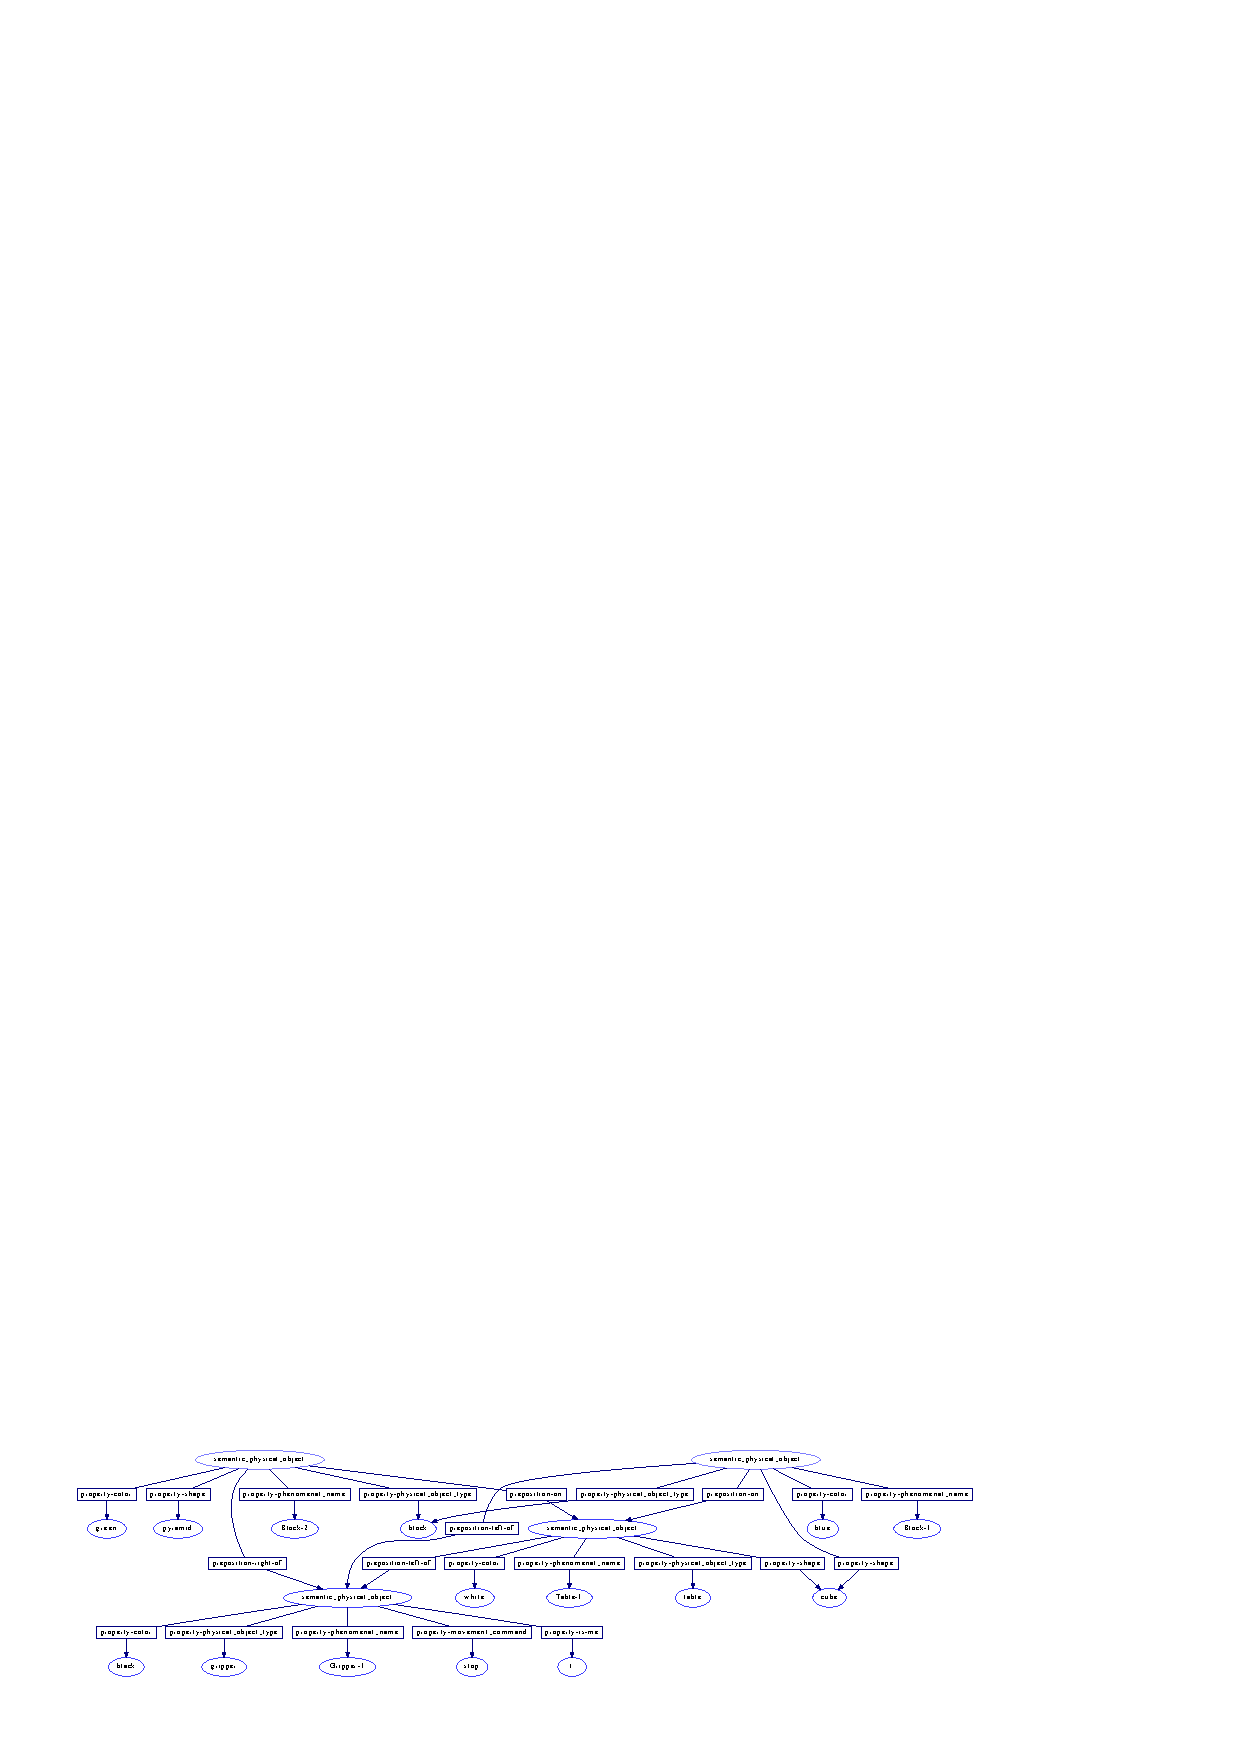
\includegraphics[width=10cm]{gfx/implemented_physical_knowledge}
\caption[The implemented physical knowledge.]{The implemented physical
  knowledge.}
\label{figure:implemented_physical_knowledge}
\end{figure}

\section{Implemented Reflective Knowledge}

{\mbox{\autoref{figure:implemented_reflective_knowledge}}} shows the
implemented reflective knowledge.
\begin{figure}

\includegraphics[width=10cm]{gfx/implemented_reflective_knowledge}
\caption[The implemented reflective knowledge.]{The implemented
  reflective knowledge.}
\label{figure:implemented_reflective_knowledge}
\end{figure}

\section{Implemented Semantic Event Knowledge-Base}

{\mbox{\autoref{figure:implemented_semantic_event_knowledge_base}}} shows the
implemented semantic event knowledge base.
\begin{figure}
\includegraphics[width=10cm]{gfx/implemented_semantic_event_knowledge_base}
\caption[The implemented semantic event knowledge base.]{The
  implemented semantic event knowledge base.}
\label{figure:implemented_semantic_event_knowledge_base}
\end{figure}

\section{Implemented First-order Resource Activator}

{\mbox{\autoref{figure:implemented_first_order_resource_activator}}}
shows the implemented first-order resource activator.
\begin{figure}
\includegraphics[width=10cm]{gfx/implemented_first_order_resource_activator}
\caption[The implemented first-order resource activator.]{The
  implemented first-order resource activator.}
\label{figure:implemented_first_order_resource_activator}
\end{figure}

\section{Implemented First-order Planning Machine Knowledge}

{\mbox{\autoref{figure:implemented_planning_machine_knowledge}}} shows
the implemented first-order planning machine knowledge.
\begin{figure}
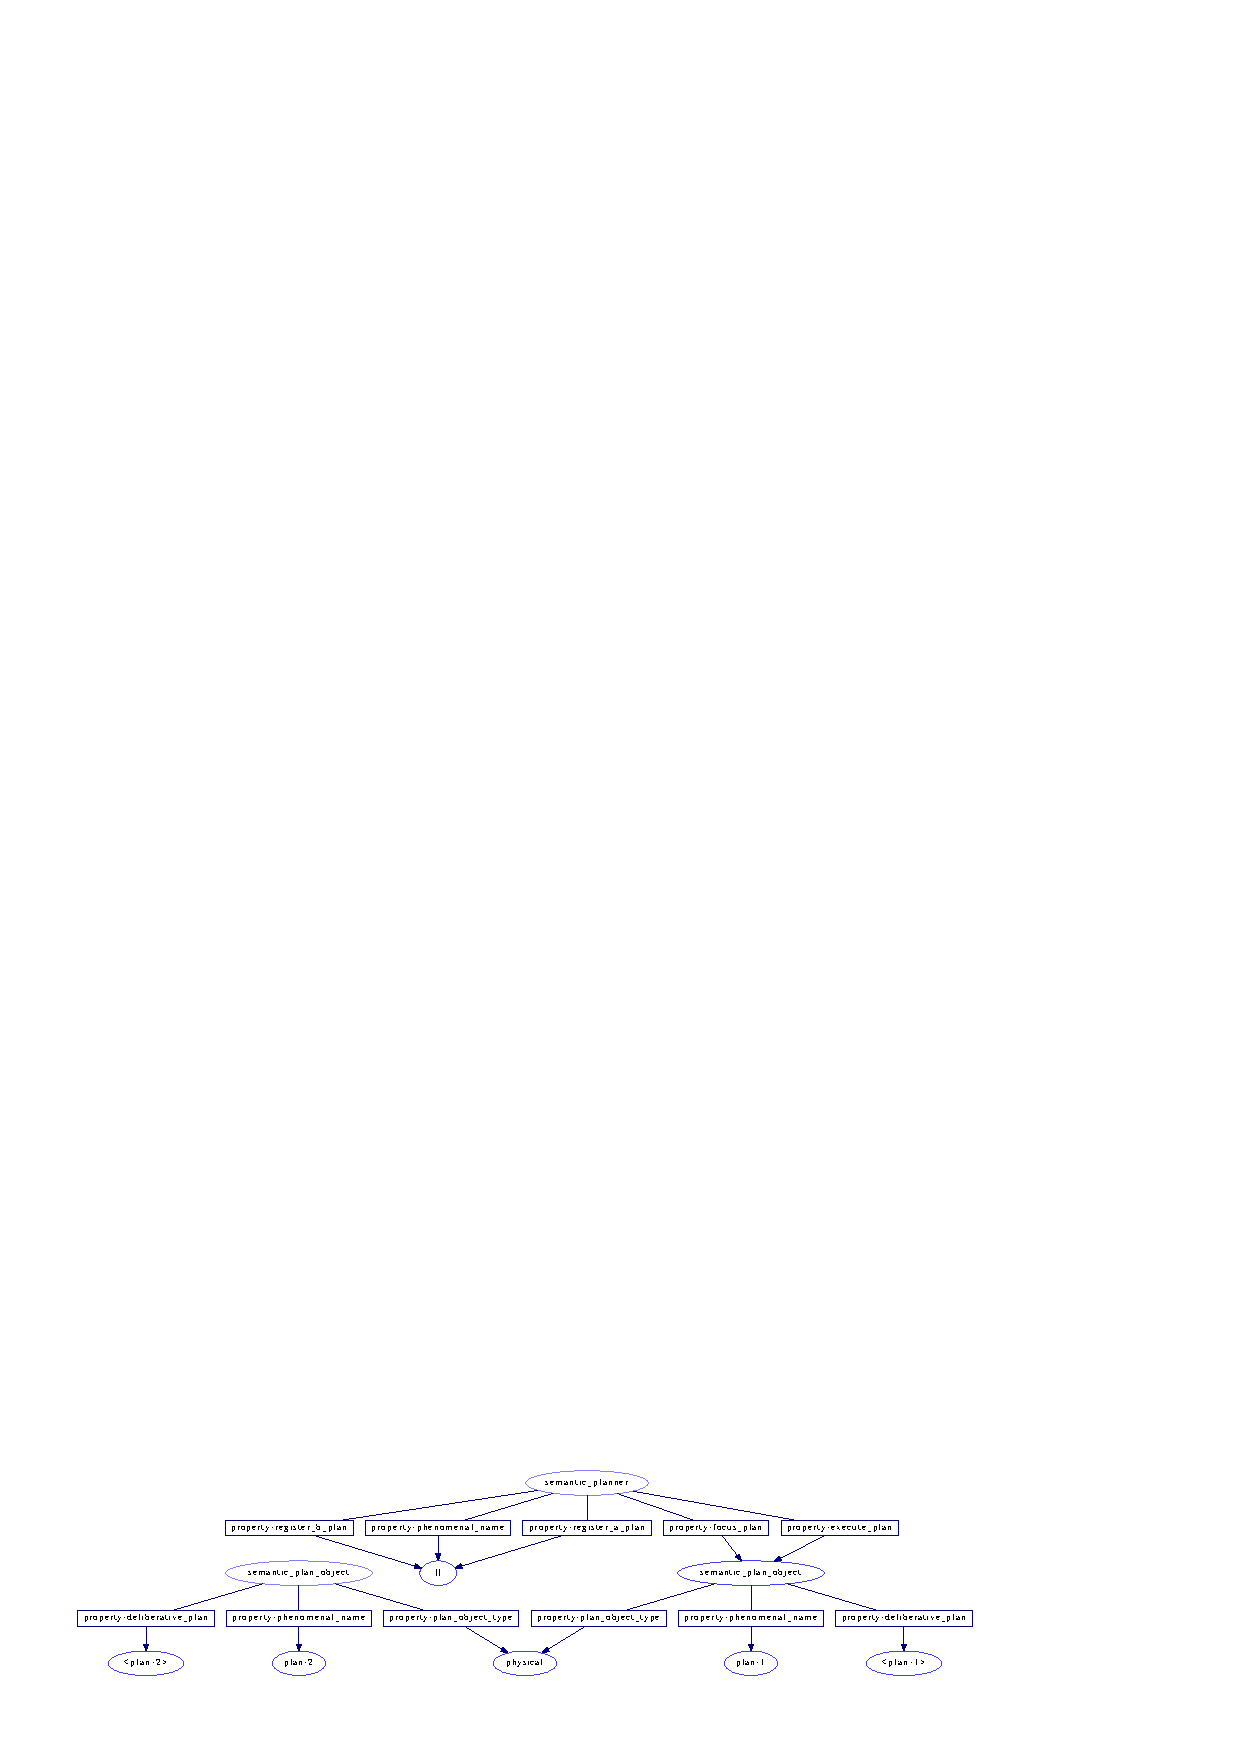
\includegraphics[width=10cm]{gfx/implemented_planning_machine_knowledge}
\caption[The implemented first-order planning machine knowledge.]{The
  implemented first-order planning machine knowledge.}
\label{figure:implemented_first_order_planning_machine_knowledge}
\end{figure}

\section{Implemented First-order Plan Activator}

{\mbox{\autoref{figure:implemented_first_order_plan_activator}}} shows
the implemented first-order plan activator.
\begin{figure}
\includegraphics[width=10cm]{gfx/implemented_first_order_plan_activator}
\caption[The implemented first-order plan activator.]{The implemented
  first-order plan activator.}
\label{figure:implemented_first_order_plan_activator}
\end{figure}

\section{Implemented Second-order Resource Activator}

{\mbox{\autoref{figure:implemented_second_order_resource_activator}}}
shows the implemented second-order resource activator.
\begin{figure}
\includegraphics[width=10cm]{gfx/implemented_second_order_resource_activator}
\caption[The implemented second-order resource activator.]{The
  implemented second-order resource activator.}
\label{figure:implemented_second_order_resource_activator}
\end{figure}


%************************************************
\chapter{The Mind Monitor Application}
\label{chapter:the_mind_monitor_application}
%************************************************

In order to control the SALS model of mind, a mind monitoring
application called \emph{MindMon} has been implemented.  MindMon is
based on abstract physical world and reflective thinking components
that allow reflective thinking layers to be interchanged with
different $\text{reflective}^0$ physical layers.  In this dissertation
I focus on a block building domain in order to demonstrate
second-order reflective learning to plan, but other more complex
physical domains have also been developed within SALS such as the
IsisWorld physical simulator described by \cite{smith:2010}, where
MindMon allows attaching multiple reflective thinking models to a
shared $\text{reflective}^0$ physical layer, a type of simulation that
assumes a more complex subjective philosophy of mind that is not
assumed in the non-subjective model described in
{\mbox{\autoref{part:the_model}}} of this thesis.
{\mbox{\autoref{figure:implemented_mindmon}}} shows the implemented
MindMon application.
\begin{figure}
\hspace*{-1cm}\includegraphics[width=13cm]{gfx/implemented_mindmon}
\caption[The implemented mind monitoring application, MindMon.]{The
  implemented mind monitoring application, MindMon, shown here with
  the simple block building domain and the reflective thinking layers
  described in this dissertation.}
\label{figure:implemented_mindmon}
\end{figure}

\section{The Physical Knowledge-Base}

The block building domain is a simulation based on two-dimensional
ridid-body physical laws, including floating point numerical
representations for object positions, velocities and accellerations.
These numerical representations and the processes that manipulate them
are part of the $\text{reflective}^0$ physical layer of the model, but
in order to focus the efficiency of the procedural reflection, a much
simpler relational graph representation has been specifically
represented in semantic frame-based objects in a semantic
knowledge-base, referred to as the \emph{physical knowledge-base}.
The physical knowledge-base includes objects with shapes, colors, and
multiple prepositional spatial relationships.
{\mbox{\autoref{figure:implemented_physical_knowledge}}} shows the
implemented physical knowledge.
\begin{sidewaysfigure}
\begin{center}
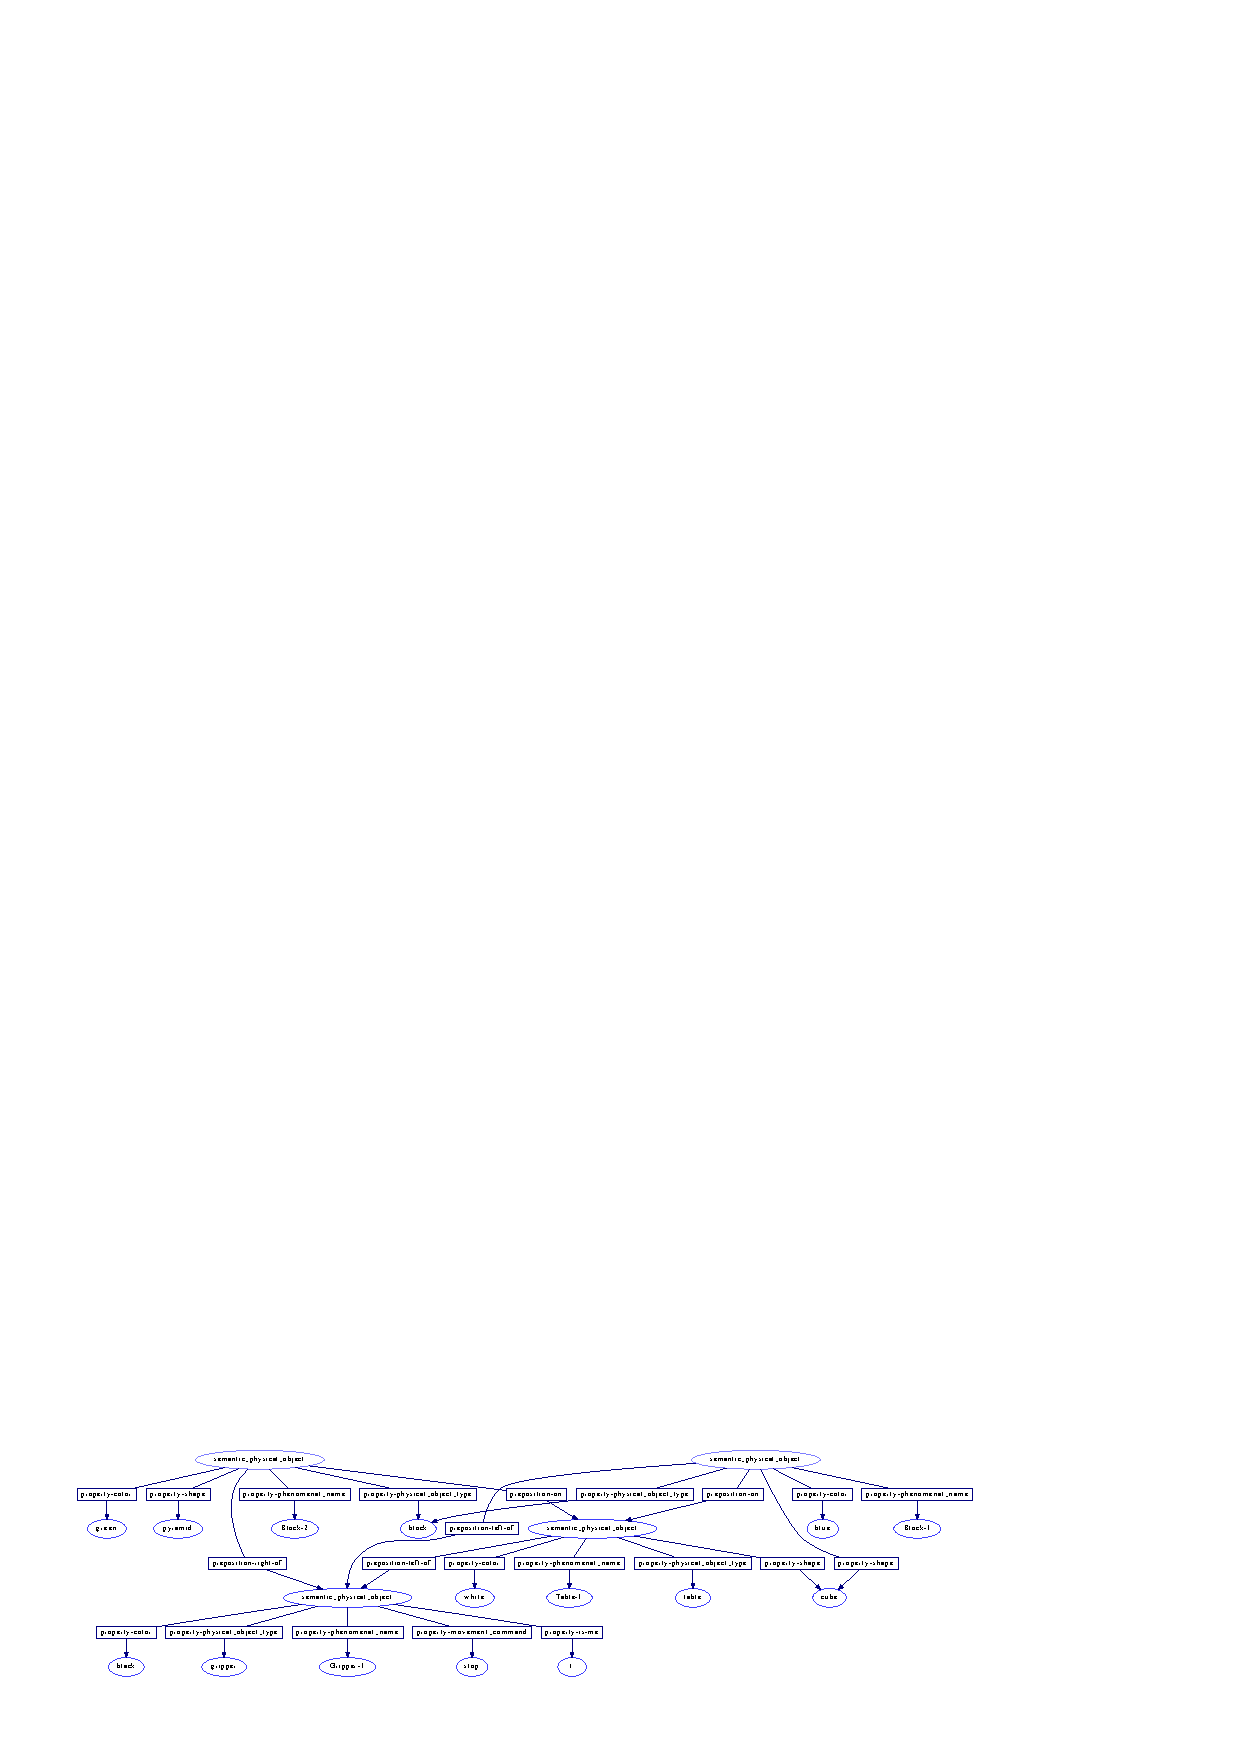
\includegraphics[width=24cm]{gfx/implemented_physical_knowledge}
\end{center}
\hspace{4cm}\parbox{15cm}{\caption[The implemented physical
    knowledge-base.]{The implemented physical
    knowledge-base.}\label{figure:implemented_physical_knowledge}}
\end{sidewaysfigure}

\section{Semantic Event Knowledge-Base}

%{\mbox{\autoref{figure:implemented_semantic_event_knowledge_base}}} shows the
%implemented semantic event knowledge base.
%\begin{figure}
%\includegraphics[width=10cm]{gfx/implemented_semantic_event_knowledge_base}
%\caption[The implemented semantic event knowledge base.]{The
%  implemented semantic event knowledge base.}
%\label{figure:implemented_semantic_event_knowledge_base}
%\end{figure}

{\mbox{\autoref{figure:implemented_reflective_event_knowledge_base}}}
shows the implemented semantic event knowledge base.
\begin{figure}
\includegraphics[width=10cm]{gfx/implemented_reflective_event_knowledge_base}
\caption[The implemented semantic event knowledge base.]{The
  implemented semantic event knowledge base.}
\label{figure:implemented_reflective_event_knowledge_base}
\end{figure}

%\section{IsisWorld First-order Resource Activator}

%{\mbox{\autoref{figure:implemented_isisworld_first_order_resource_activator}}}
%shows the implemented semantic event knowledge base.
%\begin{figure}
%\includegraphics[width=10cm]{gfx/implemented_isisworld_first_order_resource_activator}
%\caption[The implemented semantic event knowledge base.]{The
%  implemented semantic event knowledge base.}
%\label{figure:implemented_isisworld_first_order_resource_activator}
%\end{figure}


\section{First-order Resource Activator}

{\mbox{\autoref{figure:implemented_first_order_resource_activator}}}
shows the implemented first-order resource activator.
\begin{figure}
\includegraphics[width=10cm]{gfx/implemented_first_order_resource_activator}
\caption[The implemented first-order resource activator.]{The
  implemented first-order resource activator.}
\label{figure:implemented_first_order_resource_activator}
\end{figure}

\section{First-order Planning Machine Knowledge}

{\mbox{\autoref{figure:implemented_planning_machine_knowledge}}} shows
the implemented first-order planning machine knowledge.
\begin{figure}
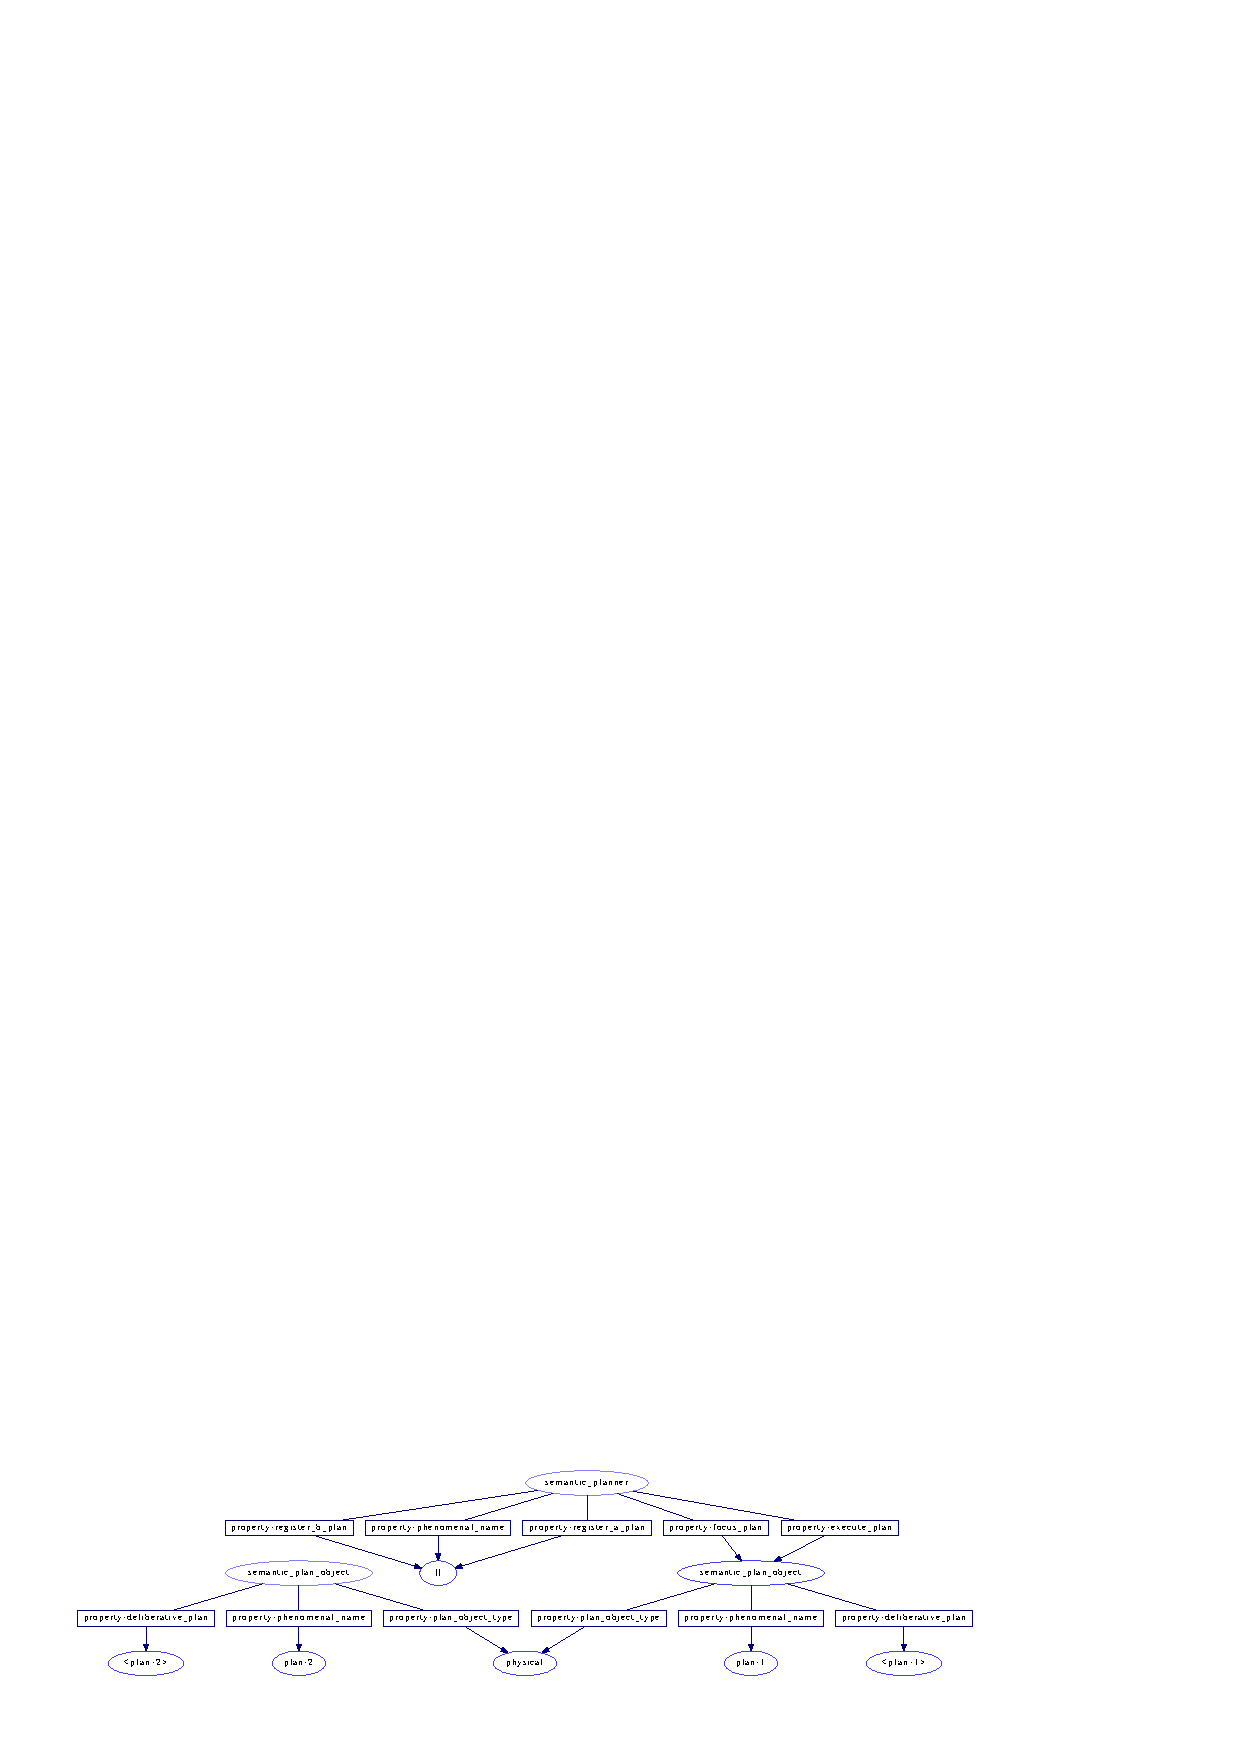
\includegraphics[width=10cm]{gfx/implemented_planning_machine_knowledge}
\caption[The implemented first-order planning machine knowledge.]{The
  implemented first-order planning machine knowledge.}
\label{figure:implemented_first_order_planning_machine_knowledge}
\end{figure}

\section{First-order Plan Activator}

{\mbox{\autoref{figure:implemented_first_order_plan_activator}}} shows
the implemented first-order plan activator.
\begin{figure}
\includegraphics[width=10cm]{gfx/implemented_first_order_plan_activator}
\caption[The implemented first-order plan activator.]{The implemented
  first-order plan activator.}
\label{figure:implemented_first_order_plan_activator}
\end{figure}

\section{Second-order Resource Activator}

{\mbox{\autoref{figure:implemented_second_order_resource_activator}}}
shows the implemented second-order resource activator.
\begin{figure}
\includegraphics[width=10cm]{gfx/implemented_second_order_resource_activator}
\caption[The implemented second-order resource activator.]{The
  implemented second-order resource activator.}
\label{figure:implemented_second_order_resource_activator}
\end{figure}


%*****************************************
\chapter{Related Implementations}
\label{chapter:related_implementations}
%*****************************************

\section{HACKER}

A good precedent for reflective debugging responses to catalogs of
failures is \emph{HACKER}, one of the first reflective planning and
debugging models, written by \cite{sussman:1973}.  [complete]

\section{EM-ONE}

\cite{singh:2005} provided \emph{EM-ONE}, a most recent example of an
extension of HACKER that reasons about a more complicated
three-dimensional physical and social block building domain.
[complete]


%\include{chapters/learning_to_accomplish_goals}
%%************************************************
\chapter{Problems to Solve}\label{ch:problems_to_solve}
%************************************************

\section{Build a Reflective Knowledge Processing System}



\section{Use Reflective Representations for Better Models of Learning}

\subsection{Tracing Knowledge Provenance for Credit Assignment of Success or Failure}

\section{Better Models for Reflectively Controlling Inductive Bias in Learning}


%%*****************************************
\chapter{Theory and Alternatives}\label{ch:theory_and_alternatives}
%*****************************************


%%*****************************************
\chapter{A System}\label{ch:a_system}
%*****************************************


%%*****************************************
\chapter{Experiments}\label{ch:experiments}
%*****************************************

\section{Blocks World as a Simple Real-Time Symbolic Control Problem Domain}

\begin{figure}[bth]
  \center
  \includegraphics[width=11cm]{gfx/blocks_world_screenshot-1}
  \caption[Blocks world is a simple real-time symbolic control problem.]{Blocks world is a simple real-time symbolic control problem that we use to demonstrate our reflective control learning theory.}
  \label{fig:blocks_world_screenshot-1}
\end{figure}

I use blocks world, a canonical toy AI problem, in order to demonstrate my example of reflectively learning to plan.
See Figure~\ref{fig:blocks_world_screenshot-1} for a screenshot of my blocks world problem physical simulation.

\begin{table}
  \myfloatalign
  \begin{tabularx}{\textwidth}{XllX}
    & [Gripper-1 is me] & [Gripper-1 movement\_command []] & \\
    & [Gripper-1 is-a gripper] & [Gripper-1 color black] & \\
    & [Gripper-1 is-holding []] & [Block-1 is-a block] & \\
    & [Block-1 color brown] & [Block-1 shape cube] & \\
    & [Block-1 on Table-1] & [Block-1 left-of Gripper-1] & \\
    & [Block-2 is-a block] & [Block-2 color blue] & \\
    & [Block-2 shape cube] & [Block-2 on Table-1] & \\
    & [Block-2 right-of Gripper-1] & [Block-3 is-a block] & \\
    & [Block-3 color green] & [Block-3 shape pyramid] & \\
    & [Block-3 right-of Gripper-1] & [Table-1 is-a block] & \\
    & [Table-1 color white] & [Table-1 shape cube] & \\
    & [Table-1 left-of Gripper-1] & &
  \end{tabularx}
  \caption[Blocks world agent perceptual input.]{Blocks world agent perceptual input.}
  \label{tab:blocks_world_agent_perceptions}
\end{table}

See Table~\ref{tab:blocks_world_agent_perceptions} for an example set of perceptual input that corresponds with the physical situation shown in Figure~\ref{fig:blocks_world_screenshot-1}.

\section{Working in a World of Building Blocks}

In his PhD thesis, Terry Winograd worked in the world of building
blocks \citep{winograd:1970}.  This program maintained traces of its
goals and subgoals, which enabled it to answer questions about why it
performed certain actions.  This system worked because it stored
goals.

Knowing the goal state of the computation is important, and we do not
ignore this aspect in tracing the deliberative layer.  Our system is
able to answer these sorts of questions, as this simply requires
climbing the stack of mental resource activations, but when debugging
the deliberative process, it is helpful to not only know the ending
point of computation but also the means toward that end.

\section{Terry Winograd's SHRDLU and Goal Tracing}

I am building upon what was learned from Winograd's thesis
\citep{winograd:1970} in terms of using traces of the deliberative
process as well as using a semantic model of the world in order to
understand communications between agents.  I have chosen to use a
simpler and more direct language interface between agents that refers
more directly to the semantic information and mental processes
involved.

\section{Why Not Work Within a Building Blocks Domain?}

The building blocks approach is a good precedent.  However, there are
many problems with only demonstrating a solution on a toy problem.
First, an approach demonstrated to solve a small problem, often do not
scale to larger problem domains of similar complexity.  So, we feel
that it is important to show the same reflective approach to learning
can also be applied to a domain with a much larger state space than
the toy blocks world problem.  We then, show the theoretical gains of
our approach by using the canonical model, and now we show that our
model does scale to larger problem domains of similar complexity.  See
\cite{smith:2010} for a discussion of the benefits of approaching the
social commonsense reasoning problem with a physical simulation of a
kitchen.

We have conscripted our domain of object types in the kitchen, such
that it is currently comparable to the number of object types that
Winograd used in his thesis.  Our object types do have different ways
that they may be used, which is a small addition of complexity.
Although we do not introduce many of the complexities of ontological
reasoning, a common approach to commonsense reasoning, e.g. Cyc
\citep{lenat:1990}, our system demonstrates an important new approach
to commonsense reasoning that grounds learning by being told in the
domain of goal-oriented reasoning, which allows organizing and
debugging knowledge in terms of what goals it is useful for
accomplishing.

\section{A Physical Simulation of a Kitchen as a Social Commonsense Reasoning Domain}

\begin{figure}[bth]
  \center
  \includegraphics[width=11cm]{gfx/mindmon-isis_world-screenshot-1}
  \caption[Isis World is a larger real-time symbolic control
    problem.]{Isis World is a larger real-time symbolic control
    problem that we use to demonstrate scaling of our reflective
    control learning theory to larger state spaces and slightly more
    complicated problems.}
  \label{fig:mindmon-isis_world-screenshot-1}
\end{figure}

We tested our cognitive architecture learning in the context of a
social commonsense reasoning domain with parents that teach children
as they attempt to accomplish cooking tasks in a kitchen.  See
\cite{morgan:2011} for details about our six-layered reflective model
of social and moral reasoning.  Kitchens are a good example of a rich
learning environment for children \citep{dewey:1907}.  Kitchens are
ubiquitous across cultures.  They have a clear production goal, food.
They involve many many mental realms: math, physics, chemistry,
thermodynamics, natural language, social, family, imprimer learning,
children, parents, concurrent planning, etc.

See Figure~\ref{fig:mindmon-isis_world-screenshot-1}.

\cleardoublepage\part{Conclusion}\label{part:conclusion}
%%*****************************************
\chapter{Results}\label{ch:results}
%*****************************************


\section{Reflective Knowledge Substrate}


\subsection{General Parallelism and Concurrency}

My system is built to handle concurrent parallel processes on
multi-core operating systems.  In this section, I test how efficient
my implementation of concurrency performs on a number of standard
concurrency timing tasks.  In an ideal situation, given $N$ processor
core working on independenct problems, I should get a factor of $N$
speedup.  Because multiple core processors share memory resources this
ideal is never actualized, so we test our implementations performance
by developing appropriate metrics.

\subsection{Program as Data}

In systems where the program is data, a bottleneck in writing programs
that write programs is the efficiency of the run-time compiler.  In
this section we test the relative performance of our compiler in
our-time system.

\section{Layered Reflective Problem Solving}

In this section, I evaluate how well different configurations of my
learning system accomplishes a range of goals in the blocks world
environment.

\subsection{Comparison between Learned Reactions and Planning}

I evaluate how adding or removing reflectively learning to plan
changes the performance of the blocks world goal accomplishment
metric.

\subsection{Analogy between Physical Goals and Planning Goals}

I evaluate how adding or removing the second layer of reflectively
learning to plan changes the performance of the blocks world goal
accomplishment metric.

\section{Learning by Credit Assignment}

\subsection{Tracing Knowledge Provenance for Credit Assignment of Success or Failure}

I evaluate how tracing causality of knowledge provenance can improve
learning performance according to the blocks world goal accomplishment
metric.


%*****************************************
\chapter{Future}\label{ch:future}
%*****************************************

\subsection{Recursive Loops and Infinite Recursive Tracing Descent}

If the focus on the tracing is controlled carefully, these potential
loops can be avoided.  How to detect and control these potential loops
is an interesting area of future automatic debugging research in
reflective control.

\subsection{Potential Future Uses for Low-Level Tracing}

Lower level objects maybe be interesting to focus on for research in
automatic abstraction and simulation of system components.  Optimizing
compilers could benefit from this area of future research.  E.g.
focusing on the CPU object could help to develop better run-time
register allocation models.

\subsection{Why Should You Use This Radically New Language?}

Because the language is very similar to Lisp, it has proven to be easy
for both expert and novice programmers to learn.  This has been my
experience with the four undergraduates that have worked within the
language, who learned it quickly, started writing their own macros to
facilitate their style, and one even made additions to the core
algorithms.

\section{Dealing with Noise in Agent Communication}

\begin{figure}[bth]
  \center
  \includegraphics[width=10cm]{gfx/communication_theory}
  \caption[A mathematical theory of communication]{A mathamtical
    theory of communication~\citep{shannon:1959}.}
  \label{fig:communication_theory}
\end{figure}

Our cognitive theory holds with or without the presence of noise.
Communication between agents in our implementation occurs across a
noiseless communication channel.  If one wishes to include a theory of
noisy communication channels, Shannon's mathmematical theory of
communication~\citep{shannon:1959} could be applied as an extension to
our basic theory.




%************************************************
\chapter{Evaluation}
\label{chapter:evaluation}
%************************************************

The primary contribution of this thesis is a recursive implementation
of a reflective planning layer that controls a deliberative planning
process.  Because of the recursive nature of this implementation, a
super-reflective layer is also used to control and learn about the
reflective planning process.  The benefit of adding each additional
reflective layer is that more can be learned from each deliberative
failure by adding each additional reflective layer, but there is a
computational trade-off in that each additional reflective layer also
increases the computational complexity of the overall architecture.
This chapter evaluates the Emotion Machine cognitive architecture
contribution of this thesis by measuring the computational complexity
introduced by adding additional reflective planning layers to the SALS
deliberative planning process.

The key to beginning to think about the computational complexity in a
given planning layer of the SALS cognitive architecture is in
considering the perceptual inputs to that layer.  The perceptual
inputs to a planning layer determine the complexity of the goals that
the planner can attempt to achieve as well as the complexity of the
causal models that are constructed for a given a rule-learning
algorithm.  There are two different types of inputs to a SALS planning
layer from the layer below:
\begin{packed_enumerate}
\item{Procedurally Reflective Event Streams}
\item{Direct Read Access}
\end{packed_enumerate}
The first, procedurally reflective event streams, is the basis of the
asynchronous learning from experience that was discussed in detail in
{\mbox{\autoref{chapter:learning_asynchronously_from_experience}}}.
To briefly review, learning from experience asynchronously abstracts a
small subset of all possible partial states from a stream of events
that represent changes that have occurred in the knowledge base that
the planning layer is trying to control.  These abstracted partial
state events are woven together with resource activation and
completion events through a rule-learning algorithm to learn abstract
hypothetical models of resource executions in the layer below.  These
hypothetical models can be used by the planning layer to imagine the
effects of plans before they are executed.  The second type of input
to a planning layer, direct read access, allows an executing plan to
access the real-time state of the knowledge base that it is trying to
control.  The important thing to realize about both of these different
methods of accessing and referring to the knowledge base in the layer
below is that both of these methods work exclusively through a small
subset of possible partial state abstractions.
{\mbox{\autoref{chapter:learning_from_being_told_natural_language_plans}}}
describes two specific types of these partial state abstractions that
can be perceived by the planning layer: (1) the ``relationship''
expression, and (2) the ``property'' expression.  The fact that all
perceptual input to a planning layer is limited to these specific
types of partial state abstractions limits the complexity of the
control problem that the planning layer confronts.  For example,
because of the simplicity of the included partial states, the SALS AI
cannot directly pursue a single goal to create a stack of three
blocks.  Instead, the deliberative layer of the SALS AI must be
instructed, by either a user or the reflective layer, to pursue two
goals composed of these simpler partial states to make a plan to stack
three blocks: (1) ``Block-1 to be on Block-2'' and (2) ``Block-2 to be
on Block-3.''  The important point is not that the abstracted partial
states are currently simple but instead that the planning layer is
\emph{limited} to perceiving its problem domain through partial state
abstractions that reduce the complexity of the problem domain to a set
of symbolic reifications that either exist or do not exist in the
control domain.

The number of partial states that are abstracted from any given
knowledge base depends primarily on the structure of the knowledge
within that knowledge base and whether or not this structure contains
the types of partial states that the SALS AI is prepared to abstract.
The partial states that are currently included in the SALS AI are
meant to be both specific enough to handle the simple types of
meaningful relationships that have been engineered to exist in each
knowledge base while being general enough to leave room for those
serendipitous abstractions that have not been engineered but may still
end up being useful to the rule-learning algorithm in building causal
models of resource executions.
{\mbox{\autoref{table:frames_slots_partial_states}}} shows how the
sizes of the knowledge bases in the layers of the SALS AI relate to
the numbers of partial states that are abstracted from these knowledge
bases by the layers above.
\begin{table}
\centering
\begin{tabular}{|l|c|c|}
\hline
\emph{Knowledge Base}     & \emph{Frames}  & \emph{Partial States Abstracted}  \\
\hline
Learned Reactive Physical & 6              & 174             \\
\hline
Deliberative Plan         & 120            & 122             \\
\hline
Reflective Plan           & 224            & 103             \\
\hline
Super-Reflective Plan     & 208            & {\scriptsize{\emph{N/A}}} \\
\hline
\end{tabular}
\caption[A comparison of the sizes of knowledge bases in the layers of
  the SALS AI to the numbers of partial states that are abstracted
  from these knowledge bases.]{A comparison of the sizes of knowledge
  bases in the layers of the SALS AI to the numbers of partial states
  that are abstracted from these knowledge bases.  Notice that the
  number of partial states abstracted from any given knowledge base is
  not directly a function of the number of frames in the knowledge
  base.  For example, the learned reactive physical knowledge base
  contains very few frames with a highly interconnected structure that
  contains many of the types of partial states that SALS is designed
  to abstract, while the plan knowledge bases contain a relatively
  large number of frames with fewer and more sparse relationships that
  result in fewer abstracted partial states.  The super-reflective
  layer is currently the highest layer in the SALS AI, so no partial
  states are currently abstracted from the super-reflective plan
  knowledge base.}
\label{table:frames_slots_partial_states}
\end{table}
Notice that the total number of partial states that are abstracted
from any given knowledge base is not directly a function of the number
of frames in that knowledge base.  For example, the learned reactive
physical knowledge base contains relatively few frames with a highly
interconnected structure that contains many of the types of partial
states that SALS is designed to abstract, while the plan knowledge
bases contain a relatively large number of frames with fewer and more
sparse relationships that result in fewer abstracted partial states.
This table shows that the number of partial states, which are the
perceptual input to each planning layer in the SALS AI, actually
decreases as subsequent layers of reflective planning are added to the
SALS AI.  In general, this rule must not always hold as planning
layers may become more interconnected, depending on the experience of
the AI.  Also, depending on the types of additional partial states
that may be added to the architecture in the future, the number of
partial state abstractions may grow intractably.  In general, the
number of perceptual inputs to any given planning layer is a control
problem in itself, which is not yet handled in the SALS AI, but for
the current state of the architecture, the number of perceptual inputs
to subsequently higher layers of reflective control grows
sub-linearly.

\section{Complexity of Learning from Being Told}

Knowledge in a SALS planning layer includes plans, goals, a planner,
and other knowledge used in the planning process.  In addition to the
planning objects, knowledge in a planning layer includes references to
knowledge in the layer below.  Keeping clear distinctions between
knowledge in different layers is critical to reducing the potential
complexity of the SALS architecture.  For example, while the
deliberative plan knowledge base references physical knowledge in the
learned reactive physical knowledge base, the deliberative plan
knowledge does not actually contain physical knowledge.  Instead, the
deliberative plan knowledge base contains symbolized reifications of
potential partial states of the physical knowledge base.
{\mbox{\autoref{figure:deliberative_physical_partial_state_reification}}}
shows a simple example of a deliberative goal that refers to a
potential partial state of the physical knowledge base and how this
partial state is symbolically reified in the deliberative layer.
\begin{figure}
\centering
\includegraphics[width=10cm]{gfx/deliberative_physical_partial_state_reification}
\caption[Deliberative physical partial state
  reification.]{Deliberative physical partial state reification.  (A)
  A visualization of the idea that a deliberative goal object can
  refer to a potential partial state of the physical knowledge base.
  (B) The actual representation of a deliberative goal object that has
  a symbolic ``partial-state'' property, the symbolic phrase, ``A cube
  is on a pyramid,'' being a reference to the potential physical
  partial state visualized in (A).  Each planning layer is limited to
  reflecting upon reified symbols that refer to partial states in the
  layer below and not the complexity of the partial states
  themselves.}
\label{figure:deliberative_physical_partial_state_reification}
\end{figure}
Because deliberative knowledge only contains symbols that refer to
physical partial states, this allows the deliberative layer to ignore
the internal details of the physical partial state and simply treat
the goal symbolically.

{\mbox{\autoref{figure:meta_meta_knowledge}}} shows a visualization of
an example of reflective knowledge that references potential
deliberative knowledge, while this potential deliberative knowledge
references potential physical knowledge.
\begin{figure}
\centering
\includegraphics[width=12cm]{gfx/meta_meta_knowledge}
\caption[A visualization of a reflective partial state with references
  to potential knowledge in the layers below.]{A visualization of a
  reflective partial state with references to potential knowledge in
  the layers below.  Although this reflective knowledge is visualized
  as a hyper-graph that includes deliberative and physical knowledge,
  all deliberative and physical knowledge is actually symbolically
  reified in the reflective partial state.  This is not a
  visualization of deliberative knowledge or physical knowledge.  This
  is a visualization of reflective knowledge.}
\label{figure:meta_meta_knowledge}
\end{figure}

\section{The Interpretation Process in Three Layers}

\begin{enumerate}
\item{\emph{Physical Partial State}: ``A pyramid is on a cube.''}
\item{\emph{Deliberative Partial State}: ``A deliberative planner is
  focusing on a plan that is hypothesized to cause a cube to be on a
  pyramid.''}
\item{\emph{Reflective Partial State}: ``A reflective planner is
  focusing on a plan that is hypothesized to cause a deliberative
  planner to be focusing on a plan that is hypothesized to cause a
  cube to be on a pyramid.''}
\end{enumerate}

has the potential to be more complex and thus more difficult to reason
about than the knowledge in the layers below that knowledge.  For
example, a partial state of the physical problem domain can be a
simple relationship such as ``a pyramid being on a cube.''  Since the
deliberative layer contains meta-physical knowledge, or ``knowledge
about physical knowledge,'' a simple deliberative partial state could
be that ``a deliberative plan fails to accomplish the goal for a cube
to be on a pyramid.''  This deliberative knowledge appears at first
glance to be more complex than the physical knowledge that it is about
because it contains, in some sense, the physical knowledge as well as
additional relationships between this physical knowledge and a plan
and a goal.  Further, the reflective layer contains meta-meta-physical
knowledge, so a piece of reflective knowledge could be that ``a
reflective plan fails to avoid the negative goal of a deliberative
plan failing to achieve the goal of a cube being on a pyramid.''
{\mbox{\autoref{figure:meta_meta_knowledge}}} shows a visualization of
this example of meta-meta-knowledge with a reflective partial state
that references a deliberative partial state that references a
physical partial state.
\begin{figure}
\centering
\includegraphics[width=12cm]{gfx/meta_meta_knowledge}
\caption{Meta-meta-knowledge of (A) a reflective partial state that
  references (B) a deliberative partial state that references (C) a
  physical partial state.}
\label{figure:meta_meta_knowledge}
\end{figure}
{\mbox{\autoref{table:meta_meta_knowledge_complexity}}} shows the
computational complexity of evaluating each one of these increasingly
complex forms of knowledge.  The phrase, ``a cube is on a pyramid,''
is interpreted in the deliberative layer and results in the following
SALS program:

\begin{samepage}
\begin{Verbatim}
[exists
  [relationship block property shape 'cube'
                preposition on
                block property shape 'pyramid']]
\end{Verbatim}
\end{samepage}

\noindent The phrase, ``a deliberative planner is focusing on a plan
that is hypothesized to cause a cube to be on a pyramid,'' is
interpreted by the reflective layer and refers to a partial state of
the deliberative plan knowledge base, which results in the following
SALS program:

\begin{samepage}
\begin{Verbatim}
[exists
  [relationship planner property planner_type deliberative
                relation focus_plan
                plan property hypothesized_to_cause
                [relationship block property shape 'cube'
                              preposition on
                              block property shape 'pyramid']]]
\end{Verbatim}
\end{samepage}

\noindent The phrase, ``a reflective planner is focusing on a plan
that is hypothesized to cause a deliberative planner to be focusing on
a plan that is hypothesized to cause a cube to be on a pyramid,'' is
interpreted by the super-reflective layer and refers to a partial
state of the reflective plan knowledge base, which results in the
following SALS program:

\begin{samepage}
\begin{Verbatim}
[exists 
  [relationship planner property planner_type reflective
                relation focus_plan
                plan property hypothesized_to_cause
    [relationship planner property planner_type deliberative
                  relation focus_plan
                  plan property hypothesized_to_cause
                  [relationship block property shape 'cube'
                                preposition on
                                block property shape 'pyramid']]]]
\end{Verbatim}
\end{samepage}



\begin{table}
\centering
\begin{tabular}{|l|c|c|}
\hline
                 &Execution Nodes   &Plan Analogies    \\
                 &{\scriptsize{(Imagine/Execute)}} &{\scriptsize{(Imagine/Execute)}} \\
\hline
Deliberative     & 18/12            & 2/0              \\
\hline
Reflective       & 98/22            & 10/0             \\
\hline
Super Reflective & 348/32           & 27/0             \\
\hline
\end{tabular}
\caption{The number of execution nodes and plan analogies that were
  made interpreting a deliberative statement about physical knowledge,
  a reflective meta-knowledge statement about deliberative knowledge
  that references the same physical knowledge, and a super-reflective
  meta-meta-knowledge statement that references the same physical
  knowledge through deliberative knowledge.}
\label{table:meta_meta_knowledge_complexity}
\end{table}


\begin{table}
\centering
\begin{tabular}{|l|r|r|}
\hline
                 &Execution Nodes &Plan Analogies \\
\hline
Super Reflective & 152            & 11            \\
\hline
Reflective       & 170            & 13            \\
\hline
Deliberative     & 3003           & 240           \\
\hline
\end{tabular}

\begin{tabular}{|l|r|r|}
\hline
                 &Version Spaces &Hypotheses \\
\hline
Super Reflective &               &           \\
\hline
Reflective       &               &           \\
\hline
Deliberative     &               &           \\
\hline
\end{tabular}
\caption{The number of execution nodes and plan analogies that were
  made during in different stages of plan processing in the different
  planning layers during a planning scenario involving the super
  reflective layer interpreting and compiling a plan to ``find and
  execute a recently learned plan that avoids a negative reflective
  goal.''  The execution of the super reflective plan becomes the
  reflective planning process.  The reflective planning process
  searches through deliberative plans until it finds a plan to ``find
  and execute a recently learned plan for accomplishing a positive
  deliberative goal.''  The execution of the reflective plan becomes
  the deliberative planning process.  The deliberative planning
  process interprets and imagines a plan to ``stack a cube on a
  pyramid,'' which is hypothesized to accomplish a positive
  deliberative goal.}
\label{table:plan_interpretation_computational_complexity_of_layers}
\end{table}


\begin{table}
\centering
\begin{tabular}{|l|r|r|}
\hline
                 &Execution Nodes &Plan Analogies \\
\hline
Super Reflective & 152            & 11            \\
\hline
Reflective       & 170            & 13            \\
\hline
Deliberative     & 3003           & 240           \\
\hline
\end{tabular}

\begin{tabular}{|l|r|r|}
\hline
                 &Version Spaces &Hypotheses \\
\hline
Super Reflective &               &           \\
\hline
Reflective       &               &           \\
\hline
Deliberative     &               &           \\
\hline
\end{tabular}
\caption{The number of execution nodes and plan analogies that were
  made during in different stages of plan processing in the different
  planning layers during a planning scenario involving the super
  reflective layer interpreting and compiling a plan to ``find and
  execute a recently learned plan that avoids a negative reflective
  goal.''  The execution of the super reflective plan becomes the
  reflective planning process.  The reflective planning process
  searches through deliberative plans until it finds a plan to ``find
  and execute a recently learned plan for accomplishing a positive
  deliberative goal.''  The execution of the reflective plan becomes
  the deliberative planning process.  The deliberative planning
  process interprets and imagines a plan to ``stack a cube on a
  pyramid,'' which is hypothesized to accomplish a positive
  deliberative goal.}
\label{table:plan_interpretation_computational_complexity_of_layers}
\end{table}

%% \section{Old Stuff}

%% This dissertation consists of four contributions that work together to
%% form the SALS AI.  From the low-level virtual machine and Lisp-like
%% programming language to the reflective and super-reflective layers of
%% the Emotion Machine cognitive architecture, it is difficult to
%% evaluate all aspects of the SALS AI by a single simple metric.
%% Therefore, this chapter presents a number of different metrics that
%% are used to evaluate the four contributions:
%% \begin{packed_enumerate}
%% \item{\emph{Emotion Machine Cognitive Architecture}: The primary
%%   contribution of this thesis is a recursive implementation of a
%%   reflective planning layer that controls a deliberative planning
%%   process.  Because of the recursive nature of the implementation, a
%%   super-reflective layer is also used to control and learn about the
%%   reflective planning process.  The benefit of adding each additional
%%   reflective layer is that more can be learned from each deliberative
%%   failure by adding each additional reflective layer, but there is a
%%   computational trade-off in that each additional reflective layer
%%   also increases the computational complexity of the overall
%%   architecture.  This chapter evaluates the Emotion Machine cognitive
%%   architectural component of the SALS AI by asking the following
%%   question: What is the increase in computational complexity
%%   introduced by adding additional reflective planning layers to the
%%   basic deliberative planning process?}
%% \item{\emph{Learning from Being Told Natural Language Plans}: The
%%   ability of each planning layer in the SALS AI to interpret and
%%   imagine the effects of ambiguous natural language plans relies on a
%%   search through possible interpretations of each natural language
%%   phrase in any given plan.  This search would quickly become
%%   intractable if it were not controlled by a number of different types
%%   of low-level programmatic constraints.  Only those natural language
%%   plan interpretations that make programmatic sense according to these
%%   constraints are further considered for imagination or execution.  In
%%   practice, each low-level constraint helps to reduce the overall
%%   search complexity by varying amounts depending on the domain of
%%   control, whether the natural language plan is describing a control
%%   process for the physical, deliberative, or reflective knowledge
%%   domains.  This chapter shows empirical results that compare the size
%%   of the overall natural language plan interpretation search with and
%%   without each of these constraints for the control of each knowledge
%%   domain in the SALS AI.  This chapter also discusses the trade-offs
%%   between introducing language specific constraints, such as
%%   English-only semantics or syntax, versus purely programmatic
%%   constraints that keep the SALS natural planning language as it is
%%   currently applicable to all natural human languages.}
%% \item{\emph{Learning Asynchronously from Experience}: The ability of
%%   each planning layer in the SALS AI to asynchronously abstract the
%%   partial state events in its control knowledge domain as well as
%%   asynchronously learn rule-based causal models of resource
%%   activations of the layer below introduces two potentially
%%   problematic scaling factors for the computational complexity of the
%%   overall SALS AI.  Firstly, the number of partial states in arbitrary
%%   knowledge domains could in the worst case introduce a factorial
%%   growth with the size of the knowledge domain and the size of the
%%   partial states being abstracted.  As factorial growth would be an
%%   intractable scaling factor for the computational complexity, this
%%   chapter shows empirical evidence for the actual scaling factors for
%%   abstracting partial states from each of the control knowledge
%%   domains, including the physical, deliberative, and reflective
%%   knowledge domains.  The causal hypothesis rule-learning algorithm
%%   could potentially even have a worse scaling factor that is a
%%   multiplier on the number of partial states abstracted in the first
%%   asynchronous stage in the SALS AI's learning from experience.  This
%%   chapter will also present empirical evidence of the actual scaling
%%   factor introduced by the conjunctive rule-learning algorithm
%%   employed in learning causal models of resource activations in the
%%   SALS AI for each planning layer, including the deliberative,
%%   reflective, and super-reflective layers.}
%% \item{\emph{Virtual Machine and Programming Language}: The SALS AI is
%%   constructed on a low-level virtual machine and Lisp-like programming
%%   language that takes advantage of multithreaded and multicore CPUs.
%%   The SALS virtual machine executes concurrent bytecode processes that
%%   are called ``fibers,'' which are an abstraction of the POSIX threads
%%   provided by the underlying operating system.  In order to minimize
%%   hyperthread-specific cache-miss effects for each concurrently
%%   executing fiber, a separate memory pool is allocated for each
%%   hardware hyperthread in each CPU core in the underlying hardware
%%   platform.  The SALS virtual machine performs dynamic load balancing
%%   in order to take advantage of as many CPU cores as possible while
%%   executing multiple fibers.  Also, the SALS virtual machine includes
%%   a concurrent tricolor garbage collection algorithm that has been
%%   optimized to be used over multiple memory pools.  In a perfect
%%   symmetric multiprocessing (SMP) system, executing $N$ fibers on $N$
%%   processors should have a constant time-complexity, but modern
%%   multithreaded and multicore CPUs have shared caches between
%%   hyperthreads and cores, which makes systems based on these CPUs less
%%   than ideal SMPs.  Furthermore, mutual exclusion (mutex) locks
%%   required for garbage collection slow down garbage collection across
%%   multiple memory pools by a factor depending on the number of
%%   cross-references between pools.  This chapter empirically evaluates
%%   how the SALS virtual machine performs at minimizing these cache-miss
%%   and locking effects on an Intel Core i7 CPU, which has 4 cores, each
%%   with 2 hyperthreads, while executing various numbers of concurrent
%%   fibers.}
%% \end{packed_enumerate}

%% \section{Computational Complexity of Reflective Layers}

%% What is the increase in computational complexity introduced by adding
%% additional reflective planning layers to the basic deliberative
%% planning process?  The answer to this question is not at first obvious
%% because of the exponentially larger state-space confronted by each
%% higher planning layer.  The result is that each additional layer adds
%% a roughly linear increase in computational complexity to the overall
%% architecture.  This chapter discusses how the increased computational
%% complexity of each additional reflective planning layer is kept from
%% becoming exponential in the SALS AI.  This chapter also discusses how
%% using concurrent hardware in order to separately simulate each
%% additional reflective layer has the potential to reduce the overall
%% time-complexity of the architecture to sub-linear per additional
%% layer.

%% The SALS AI consists of 100 parallel heterogeneous resources,
%% organized into 29 agencies, which comprise the 5 layers.  The causal
%% procedurally reflective tracing features of the SALS virtual machine
%% that have been described in
%% {\mbox{\autoref{chapter:virtual_machine_and_programming_language}}}
%% allow for the run-time evaluation of each separate causally scoped
%% component of the SALS AI.  In the evaluation of the complexity of each
%% additional reflective layer, the following execution events are
%% measured:
%% \begin{packed_enumerate}
%% \item{Memory Allocation in Bytes}
%% \item{Garbage Collection in Bytes}
%% \item{Bytecode Execution Count}
%% \item{Semantic Frame Slot Mutations}
%% \item{Plan Interpretation Nodes Considered}
%% \item{Analogical Plan Matches Considered}
%% \end{packed_enumerate}
%% Each planning layer in the SALS AI can be used to specify very similar
%% types of goals.  For example, consider the following three different
%% pieces of knowledge:
%% \begin{packed_enumerate}
%% \item{``A pyramid is on a cube.''}
%% \item{``A deliberative planner has the positive goal for a pyramid to
%%   be on a cube.''}
%% \item{``A reflective planner has the positive goal for a deliberative
%%   planner to have the positive goal for a pyramid to be on a cube.''}
%% \end{packed_enumerate}
%% This is the feared, worst-case scenario that the analogical language
%% interpretation process in each subsequently higher reflective layer of
%% reasoning becomes an exponentially more difficult problem.  In
%% general, however, this is not true because reflective reasoning does
%% not and in practice often does not involve directly interpreting these
%% types of exponentially more difficult natural language interpretation
%% problems.  This is because reflective natural language plans are very
%% rarely directly about specific states of knowledge in the physical
%% knowledge base as in these examples.  Usually, reflective knowledge is
%% about much simpler partial states of the deliberative planning machine
%% that do not involve any physical knowledge at all.  For example,
%% consider the following pieces of knowledge:
%% \begin{packed_enumerate}
%% \item{``A deliberative planner is focused on a plan that has failed.''}
%% \item{``A reflective planner is focused on a plan that has failed.''}
%% \end{packed_enumerate}

%% {\mbox{\autoref{table:plan_interpretation_computational_complexity_of_layers}}}
%% shows measures of computational complexity for each planning layer in
%% SALS AI as it goes through the learning scenario presented in the
%% introduction to this dissertation.
%% \begin{table}
%% \centering
%% \begin{tabular}{|l|l|l|l|l|}
%% \hline
%%                  &Alloc &GC &BC &Mutate \\
%% \hline
%% Deliberative     &      &   &   &       \\
%% \hline
%% Reflective       &      &   &   &       \\
%% \hline
%% Super Reflective &      &   &   &       \\
%% \hline
%% \end{tabular}
%% \caption{Computational complexity of plan interpretation for each
%%   planning layer.}
%% \label{table:plan_interpretation_computational_complexity_of_layers}
%% \end{table}
%% In order to measure the increase in computational complexity
%% introduced by adding additional reflective planning layers to the
%% basic deliberative planning process,   While more can be learned from
%% each deliberative failure by adding additional reflective planning
%% layers, each additional reflective layer also increases the
%% computational complexity of the overall architecture.  First, let us
%% consider the computational complexity of the deliberative planning
%% layer.

%% The answer to this question is not at first obvious because of the
%% exponentially larger state-space confronted by each higher planning
%% layer.

%% The result is that each additional layer adds a roughly linear
%% increase in computational complexity to the overall architecture.

%% This chapter discusses how the increased computational complexity of
%% each additional reflective planning layer is kept from becoming
%% exponential in the SALS AI.

%% This chapter also discusses how using concurrent hardware in order to
%% separately simulate each additional reflective layer has the potential
%% to reduce the overall time-complexity of the architecture to
%% sub-linear per additional layer.

%% \section{Computational Scaling of Natural Language Interpretation Constraints}

%% \section{Computational Scaling of Partial State Abstraction and Rule-Learning}

%% Given that each planning layer in the SALS AI is based on perceiving
%% and acting based on the existence or non-existence of partial states
%% in the knowledge base that is being controlled by the planning layer,
%% the state-space of the control domain that is perceived and reacted to
%% by a planning layer is directly related to the number of partial
%% states that can be abstracted from this control domain.  For example,
%% if we consider that the knowledge base that is being controlled by a
%% given planning layer is represented as a graph, which is not exactly
%% correct but will suit our purposes here, the set of partial states
%% that can be abstracted from this control domain includes a subset of
%% all possible subgraphs of this graph representation.  In order to
%% avoid an intractable number of partial states being automatically
%% abstracted from a given knowledge base, the types of partial states
%% that the SALS AI abstracts are limited to the ``relationship'' and
%% ``property'' types of partial states described in
%% {\mbox{\autoref{chapter:learning_asynchronously_from_experience}}}.
%% These simple types of partial states limit the complexity



%% %\begin{equation}
%% %({2^n}-1)\left(\frac{n(n-1)}{2}\right)^{\ell}
%% %\end{equation}


%% \section{Computational Scaling of Concurrent Processing Hardware}


%% \section{old stuff}

%% \section{Boot-up and Perceive Experiment}

%% As an initial evaluation of the run-time performance of the AI, I have
%% run an experiment that simply initializes the AI and lets it perceive
%% the world over time.  The physical world does not change during this
%% experiment and the AI is not given any goals to accomplish, so this
%% experiment is a control that shows the baseline memory usage and
%% run-time performance of the cognitive architecture in its ``idling''
%% mode.  This experiment shows that the mind takes $10$ minutes to
%% initialize.  After initializing, the AI learns from its initial
%% perception and continues to attempt to detect changes in its raw
%% visual input over the next $50$ minutes.  Over the $50$ minutes of
%% continuous perception, the mind uses a highly fluctuating amount of
%% memory that stays, on average, relatively constant.  The mind is not
%% static in this experiment.  The mind contains resources that allocate
%% an average of $1.8$ megabytes per second in the built-in reactive
%% layer process of detecting visual changes in the next state from the
%% physical simulation, so that these changes may be propagated to the
%% physical knowledge of the learned reactive layer in a stream of
%% events.  Over $6$ gigabytes of memory is allocated over the entire
%% $60$ minutes of the experiment.  The mind uses an average memory
%% footprint of about $26$ megabytes over the course of the experiment.
%% The bytecode execution rate stabilizes at about $12$ thousand
%% bytecodes per second.  The concurrent processing capabilities of the
%% architecture can handle bursts of $50$ thousand bytecodes per second,
%% but this experiment simply shows that the execution rate of the
%% architecture does not slow down over time.  The entire cognitive
%% architecture exhibits stable handling of continuous processing for
%% experiments lasting over an hour, handling the allocation and garbage
%% collection of many gigabytes of memory in the process.
%% {\mbox{\autoref{figure:data/bootup_evaluation/mind_plot-Gripper-1}}}
%% shows a plotted overview of the run-time performance of the AI during
%% the boot-up and perceive experiment.  \autoref{table:bootup} on page
%% \pageref{table:bootup} shows more detailed plots for the run-time
%% behavior of each individual layer and agency within the AI.
%% %\experimentAIdatafigures[60]{bootup_evaluation}{an experiment that
%% %  boots up the AI, allowing it to continue to perceive the physical
%% %  world over time without stimulating it to achieve any goals.  This
%% %  experiment shows that the AI learns from its initial perceptions,
%% %  and when these do not change, it has nothing to learn and memory
%% %  usage is stable.}

%% \section{Deliberative Learning Experiment without Reflection}

%% The second run-time experiment that was performed with the cognitive
%% architecture does not include the reflective learning component that
%% learns hypothetical models for how the deliberative resources modify
%% the planning machine type knowledge base.  The AI is initialized,
%% which takes the same $10$ minutes as in the initial experiment.  The
%% AI is then told to execute a deliberative plan, which causes it to
%% execute a plan that attempts to stack a cube on top of a pyramid.  In
%% learning the effects of reactive resource executions on the physical
%% type knowledge bases the deliberative AI allocates $5.3$ megabytes per
%% second, while the memory footprint only grows at a rate of $90$
%% thousand bytes per second due to the learning that occurs over the
%% $60$ minutes that it takes to fail to accomplish this goal.  The AI
%% does not respond to the failure because the reflective layers are not
%% active.  The AI allocates an average of $1.2$ megabytes of memory per
%% second for the length of the experiment, which results in a total of
%% $5.4$ gigabytes over the course of the experiment.  The architecture
%% executes an average of $11$ thousand bytecodes per second over the
%% course of the experiment.  This shows that the architecture slows down
%% when more resources are active than simply the reactive perceptual
%% resources.  As deliberative learning resources become active, the
%% bytecode rate does not decrease much from the $12$ thousand bytecodes
%% per second in the control, but the overall memory allocation rate does
%% decrease by a factor of $66$\% from $1.8$ megabytes per second in the
%% control to $1.2$ megabytes per second with deliberative learning
%% enabled.
%% {\mbox{\autoref{figure:data/no_reflective_learning_evaluation/mind_plot-Gripper-1}}}
%% shows a plotted overview of the run-time performance of the AI during
%% the deliberative learning experiment with the reflective layer
%% disabled.  \autoref{table:no_reflective_learning} on page
%% \pageref{table:no_reflective_learning} shows plots of data for the
%% entire mind, each layer, as well as each agency within each layer for
%% this deliberative learning experiment.
%% %\experimentAIdatafigures[75]{no_reflective_learning_evaluation}{an
%% %  experiment with the reflective tracing of the deliberative process
%% %  disabled.  This experiment can be compared with run-time behavior of
%% %  the full AI cognitive architecture, which can learn from the failure
%% %  and initiate a second attempt at plan selection and execution.}

%% \section{Deliberative and Reflective Learning Experiment (The Full Architecture)}

%% The third run-time experiment that was performed with the cognitive
%% architecture includes both the deliberative as well as reflective
%% learning layers.  The deliberative layer learns hypothetical models of
%% the reactive resource execution effects on the physical type knowledge
%% base, while the reflective layer learns hypothetical models of the
%% deliberative resource execution effects on the deliberative planning
%% machine type knowledge base.  Although this experiment involves an
%% initial imaginative and plan selection processes in the reflective
%% layer, this experiment runs very similarly through the first $75$
%% minutes of otherwise mostly deliberative and reactive resource
%% executions.  Around minute $75$, the cognitive architecture responds
%% to the failure in the deliberative planning machine with the
%% reflective bug response, which begins another round of reflective
%% learning, imagination, and refined plan selection.  After a reflective
%% bug response, the goal is accomplished successfully around minute
%% $105$.  The experiment is allowed to run continuously after this point
%% for a total of $180$ minutes in order to show the performance of
%% baseline perceptual activity after going through the complete process
%% of deliberative and reflective learning.  Except for a blip at minute
%% $135$, which requires an extended garbage collection period, the AI is
%% otherwise stable after both layers have successfully demonstrated
%% learning.  With the addition of the reflective learning layer in the
%% final experiment the average bytecode execution rate has dropped
%% significantly, running at a factor $55$\% of the execution rate of the
%% architecture in the experiment demonstrating only deliberative
%% learning.  This experiment demonstrates the taxing demand of the extra
%% concurrent processes and memory allocation required with the
%% additional reflective learning algorithm.  However, slowing the
%% algorithm down by a factor of two with the addition of a reflective
%% layer of learning shows that the slow down is roughly linear with the
%% additional layer.  For example, in a naive approach to reflective
%% learning, an exponential increase in processing would be expected
%% because all resource executions and knowledge in the layers below
%% would be reflected upon and modelled by the reflective layer.  Because
%% the reflective learner implemented in this architecture only reflects
%% over the deliberative planning machine and not all of the processing
%% in the layers below, this architecture shows a linear slowdown with
%% the addition of reflective layers of learning.
%% {\mbox{\autoref{figure:data/reflective_learning_evaluation/mind_plot-Gripper-1}}}
%% shows a plotted overview of the run-time performance of the AI during
%% the reflective learning experiment.
%% \autoref{table:reflective_learning} on page
%% \pageref{table:reflective_learning} shows plots of data for the entire
%% mind, each layer, as well as each agency within each layer for this
%% reflective learning experiment, showing the run-time performance of
%% the full architecture.
%% %\experimentAIdatafigures[180]{reflective_learning_evaluation}{an
%% %  experiment testing the full AI cognitive architecture, including the
%% %  reflective tracing of the deliberative planning process, imagining
%% %  the potential failures of the deliberative planning machine as well
%% %  as the physical effects of physical actions.}

%% \section{No Theoretical Slowdown of Original Algorithm}

%% In order to assume that there is no theoretical slowdown of the
%% original planning algorithm when reflective learning is applied, it
%% must be assumed that the reflective implementation is an ideal
%% concurrent shared memory architecture.  In practice, the underlying
%% Funk virtual operating system slows down when more concurrent and
%% parallel tasks are executing.  This is beside the theoretical point,
%% but the following table shows a real-time test of the actual slowdown
%% experienced by the Funk operating system as different numbers of
%% parallel tasks are executed to perform a simple numerical processing
%% task.  The test was done on a dual Pentium processor computer, each
%% with ``core duo'' technology with each core implementing
%% ``hyper-threading'', which ends up appearing as eight processors to
%% the Linux operating system underlying the Funk virtual operating
%% system:

%% \vspace{5mm}
%% \begin{tabular}{ll}
%% Tasks & Real-Time (s) \\
%% 1 & 29\\
%% 2 & 36\\
%% 3 & 46\\
%% 4 & 44\\
%% 5 & 68\\
%% 6 & 67\\
%% 7 & 73\\
%% 8 & 110\\
%% \end{tabular}
%% \vspace{5mm}

%% As each additional concurrent resource in the cognitive architecture
%% begins execution, this table shows the approximate slowdown that the
%% Funk virtual machine experiences on this specific dual processor
%% hardware.



% 1. models of cognition intro
% 2. literature of cognition/ commonsense (s)
% 3. problems i will solve
% 4. theory and alternatives
% 5. a system
% 6. experiments with it
% 7. discussion (how it can integrate and expand on and changes what will happen
% 8. future


%*******************************************************
% Backmatter
%*******************************************************
\appendix
\cleardoublepage\part{Appendix}
%************************************************
\chapter{Science}
\label{chapter:science}
%************************************************

Physically objectifying problems scientifically has proved useful.
The primary utility of this understanding is that the scientist can be
replaced by another scientist and the experimental results can be
duplicated.  Arbitrary replacement of the subjective scientist implies
the potential for mechanical simulation of the physical phenomenon,
reducing the subjective scientist to a purely perceptual role.
Mechanical duplication of human labor leads to increased efficiency
and productivity.  First, steam engines were a model of autonomous
human activity.  Next, computers became the physical model of choice.
Now, various humanoid robots have included electrical motors and
computers to become closer reproductions of human physical abilities.
Thus, understanding a model of mind has become important in
duplicating more complex human physical behaviors that require
thinking.  The mechanical duplication of human thinking is the goal of
the field of AI.  Only the simplest forms of human thinking have been
coherently mechanized thus far.

\section{Object and Subject}

Causal hypotheses are used in order to predict the future occurrence
of symbolic perceptions and goals.  Through reflective thinking, plans
are constructed from causal hypotheses consistent with the past,
elaborating the necessities in the past and the results in the future.
Analogies between consistent plans can be abstracted into models of
objects.  For example, a plan that begins and ends with the same
symbolic perception could be considered an example of a ``circular''
object; thus, an analogical plan abstraction would represent a type of
object, that has multiple sides to perceive depending on the subject's
position in the plan.  Circular objects may be an important type of
object to analogically recognize because a circular object allows one
to perform actions while being able to get back to a known perceptual
symbol.  If one is in a known circular object, then one is not lost in
the sense that one can always follow the circle in order to get back
to any perceptual symbol contained within the circular plan object.
My implementation includes tools for performing analogical
abstractions and constructions of plans, but this machinery is not key
to my thesis of explaining causal reflective learning to accomplish
goals.  I include this section in the dissertation to eliminate a
potential confusion that would conflate the concept of symbol with
that of object.  Symbols are the most primitive elements available to
thinking, while objects are more complicated in that they are composed
of analogical consistencies between plans that are themselves composed
of many symbols.  Objects have multiple subjective perspectives.
Objects are static creations of a mind, based on static symbols
representing the ongoing activity in Duration.

\section{Body and World}

An intelligent mind builds models that predict the occurrence of
perceptual symbols.  Analogical thinking is used to abstract objects
and simultaneously the implied subjective perspectives on these
objects as they are manipulated.  The separation between the physical
body and the physical world is an objective form of thinking that is
fundamentally caused by goals that emphasize distinguishing bodily and
worldly goals in the causal structures of the physical perceptions.
For example, physical actions that change physical perceptions in
predictable ways are often bodily physical perceptions, i.e. moving
ones hand in front of ones face causes one to consistently see a hand.
Also, physical pain perceptions could be related to physical goals
that emphasize the static separation between the body and the world.
Understanding the static separation of the body and the world allows
for an objective form of scientific study that places the object of
study in the world outside of the effects of the body.

\section{The Dynamic as ``Out There''}

Scientists and others often view the dynamic as ``out there''.  What
this means is that the dynamic is viewed as a collection of objects,
some of which have been discovered, and many of which are still ``out
there'' and ready to be discovered.  ``Out there'' generally means
outside of the physical body and in the physical world.  To me, this
view of the dynamic as ``out there'' is grounded on a physically
objective view, which implies a subject; equivalently, one could state
that this view of the dynamic being ``out there'' could be grounded on
a subjective view, which implies objects.  In either case, the view of
objects is not mentally grounded on anything less than objects or
their implied subjects.  The mind is not an object, and, logically,
studying the mind is not a subjective task.  The scientist studies
objects to great utility, but what is often not clear are the goals
that have driven the measurement of utility with these subjective
objectifications.  The objects are taken as given to the mentality as
if the mind did not create the objects in order to think subjectively
in the first place.  The idea of objective thinking being less prone
to error than subjective thinking is purely two sides of the same
coin, and the error in both cases is in respect to the goals of the
creator of the distinction.  With every object is an implied set of
subjective perspectives, and every object and subject distinction is
useful with respect to the goals that relate to its creation and
experimentation.

One of the key distinctions between those who study the mind and
scientists is that scientists do not explicitly model the goals that
drive the creation of their objects of study, while those who model
the mind do not model an object from a subjective perspective because
the mind is not an object.  The mind is everything that exists.  A
model of the mind includes and explicitly states the goals that drive
it to create objects and their implied subjective perspectives.
Therefore, the dynamic is not ``out there'' but the dynamic is
everything that exists.  Seeing the dynamic as ``out there'' is based
on a static object and subject distinction that often carries with it
undisclosed goals for its creation.  It is therefore a mistake to see
this static object and subject distinction as an unquestionable
fundamental quality of existence.

It is an option for scientists to be aware of the goals that drive
their subjective studies of objects.  A goal is not a physical object
that a scientist can study subjectively.  A goal is part of a model of
mind; so, therefore, in order for a scientist to be aware of their
goals, he or she must understand a model of mind that allows them to
understand their chosen goals in relation to everything else that also
exists.  Without this awareness, there is a critical danger of the
blind leading the blind with the scientist not being aware of their
choice of a subjective perspective on the world.

\marginpar{\emph{Understanding this distinction replaces the role of
    the subjected victim with that of the responsible creator.}}  Most
importantly, we are not fundamentally subjected to objects; we are
instead the creators of static objects, based on many static symbolic
references to the actual dynamic ongoing activity.  This is a subtle
distinction, but understanding this distinction replaces a role of the
subjected victim of fundamentally unquestionable objects with the role
of the personally responsible creator of static objects with implied
subjective perspectives.  Understanding that objects are the static
creations of an intelligent mind is something that seems to have
escaped the explicit statement of many great scientists.  The fact
that the study of the mind is not a subjective field separates it from
all sciences.  The mind is not able to be studied scientifically for
this exact reason.  Science is based on objective and subjective
distinctions that are creations of a mind.  Studying and understanding
a model of mind is akin to understanding causality; a prerequisite
before posing a scientific hypothesis.  Therefore, the dynamic is not
``out there'' as many scientists currently believe; the dynamic is
everything that exists, all activity that is currently ongoing in
Duration, the mind.

\section{Physics}

The physicist uses an objective form of thinking in order to separate
his or her self as the subject from the object of their study.
Objectification of physical perceptions has led to the static creation
of universes, galaxies, stars, planets, humans, organs, cells,
molecules, atoms, and even the fascinating electrons, which can be
thought of as wave objects or particle objects, depending on the goals
of the subject.  In each of these studies, symbolic perceptions are
correlated into causal hypotheses and these causal hypotheses are
grouped into plans that are analogically abstracted into objects, each
different objective abstraction having different subjective
implications.  Note that objects and their implied subjective views
are static constructions caused by the goals of an intelligent mind.
The fact that the position and momentum of an electron can be
considered objectively as probability distributions is fundamentally
derived from counting symbolic perceptions and putting the resulting
numbers into ratios.  The symbolic perceptions in this task are the
closest thing to the dynamic activity of perception.  Once the dynamic
activity of perception has been reflectively symbolized, all that
remains is to manipulate the static Spatial arrangements of these
symbols.

\section{Neuroscience}

In the field of AI, there is a tendency to confuse an objective
scientific model of the brain with a model of mind, which is, among
other things, an explanation of the modelling of the object and
subject distinction.  Neuroscience is fundamentally an objective
physical science.  Neurons are one of the most important objective
discoveries of neuroscience.  Like all objective physical sciences,
the objects discovered are caused by goals.  The objective study of
neuroscience has led to distinctions between the central and
peripheral nervous systems; forebrain, midbrain, and hindbrain
divisions; cortical columns and circuits; nerves and pathways; all
composed of neurons.  The objectification of the nervous system is led
by the goals of the scientist, which are usually medical.  Recently,
the study of neuroscience has combined with psychology and AI, which
allows for studying not just the physical structure, but how this
physical structure relates to a model of mind.  How is reflective
thinking, which requires symbols, done by the brain?  This is an
interesting question, but I want to make the point that in order to
study a question like this one must not confuse a model of mind with
the physical objective model, both being necessary for posing a clear
question relating thinking and the brain.

\section{Neural Networks}

Neural networks are one of the objects created by the field of
neuroscience.  Given the physically objective assumptions of the
field, we have learned of the interactions between many different
objects related to neural networks: the brain is composed of
approximately one hundred billion neurons; chemical gradients guide
neuron growth and attrition; neurons use chemical binding and
electrical potential differences to communicate through axons to
dendrites.  There are many computational models that have been created
to explain different physical phenomena that arise from the
interactions of many neurons.  The study of neural networks is an
objective physical science, like all of neuroscience.  Neural networks
are static objective creation of a mind.

\section{Computational Neural Networks}

Computational models of biological neural networks are generally
referred to as \emph{artificial neural networks}.  Note that there is
a danger of confusion here between the initial static construction of
the neural network object and subject distinction in the mind of the
scientist and the further static construction of a computational
description of the subjective view of this object.  Since both of
these objects are static by definition, I will use the term
\emph{computational neural network} when I am specifically referring
to the simulation of the mathematical neural network object.

Computational neural network models were originally created in order
to explain the behavior of physical neurons; however, a subset of
these models that were modelled as simple linear and non-linear
algebraic equations have become popular as a subset of control and
optimization model.  These control models been found to be useful for
controlling robot arms, car braking systems, and even music
recommendation systems.

It is important to make a distinction between three ideas here: neural
networks, numerical control models, and thinking.  Thinking is the
activity that builds models of all of these phenomena, including
itself.  Algebraic control systems are symbolic models that assume
that one knows how to count, add, and multiply.  Neural networks are
an object created by physically objective neuroscience.  Because a
neural network is a physical object, it is an analogical abstraction
of plans composed of causal models that are themselves composed of
symbols that refer to physical actualities.  Note that of these three
ideas, thinking is the only one that is actual; the other two are
static models, which are created by the thinking activity.

\section{Brain and Mind}

The brain is one of the key organs that keeps humans alive.  The
nervous system is a key factor in muscular movement of the body;
perceptions, including vision, smell, touch, etc.; speech production;
language understanding; thinking, including counting, making plans,
and doing mathematical calculations.  When I say that the brain is
key, what I mean is that when the brain is damaged, these functions
are lost.  Understanding neural networks, like most neuroscientific
pursuits, is often driven by medical goals.  If a neural network is
understood in terms of how it leads to functionality, such as
thinking, then we can use this physical understanding in correlation
with a model of mind to design preventative, rehabilitative, and
augmentative approaches to neural medicine.

There is a danger at this point of becoming confused and accepting a
model in place of the the dynamic of the ongoing activity in Duration,
which requires neither symbols, objects, nor any other form of
thinking to exist.  A model of mind is a construction that is used to
think about this ongoing existence.  A model of the brain is a
construction that is based on the static physically objective
assumptions that divide bodies, organs, cells, etc.  Note that a model
of mind does not necessarily make any objective assumptions; in this
sense, a model of mind can model the exploration and creative activity
that leads to a model of the brain.  A model of the brain is a
physically objective model, and does not lead to models of thinking
because of the assumptions of purely physical objective focus.
However, regardless of focus, both examples of modelling must keep the
the dynamic of the ongoing activity as the fundamental referent for
any symbolized perceptions or causal models.  Some models may be
derivatives of others, but all models are static.


%************************************************
\chapter{Education}
\label{chapter:education}
%************************************************

%\section{Skill and Understanding}

To understand an activity in Duration is to actively maintain a causal
model of its effects.  There are many activities in Duration that are
referred to as skills that do not require understanding.  For example,
an understanding of walking is not necessary for the skillful activity
of walking to occur.  Skills are symbolic references to activities
that may be refined through symbolic repetition without having any
causal model existing for the activity.  Also, one may have an
understanding without having any symbolic skill referring to the
activity.  Often, an understanding of the activity can guide a
practice routine for refining the skill.  Coaches use an understanding
of a skill to provide instructions for practicing skills.  When skills
are practiced, the activity in Duration changes.  The understanding of
the skill does not necessarily change during the practice.  Practicing
a skill can simply lead to sub-symbolic changes to the activity that
the symbolic skill is a referent.

\section{Coaching and Teaching}

Coaching and teaching play similar roles in changing the mind of the
disciple.  The purpose of coaching is to change sub-symbolic skillful
activities, while the purpose of teaching is to give the disciple an
understanding of an activity.  The roles of coach and teacher work
well together.  For example, the master may teach the disciple an
understanding of a symbolic activity before coaching how to practice
the skill.  Often, an understanding is used as a crutch for initially
learning to practice a skill, and once the disciple has learned to
practice the skill, the understanding is no longer necessary and is
sometimes even a distraction from its mastery.

\section{Understanding and Mechanical Simulation}

If an activity is understood, then a mechanical model of the activity
can be built, allowing for the symbolic simulation of the activity.
Computers allow for the mechanical simulation of the active
maintenance of symbolic relationships in Space; computers also allow
for the simulation of causal models, allowing transitions from the
past to the future.  Therefore, computers allow for the mechanical
simulation of the understanding of an activity.  In this sense, the
existence of a mechanical simulation of the understanding of an
activity is an existence proof for the understanding of the activity.
Further, for any understanding, a mechanical simulation can be built.
Therefore, a one-to-one relationship exists between an understanding
and a mechanical simulation.

\section{Education through Neuroscience}

Education is a field that is designed to coach and teach an
understanding of skillful thinking activities.  Current technology
uses cleverly designed forms of reading and writing as the primary
tool for determining whether or not a child has learned the target
skills.  As the skills become longer and more complex, it becomes
harder for this form of linguistic evaluation to be designed by the
teacher.  Modern brain scanning technologies have begun to explore
exciting new ways to approach education of sub-linguistic symbolic
thinking.  This opens the possibility for the coaching and teaching of
pre-linguistic forms of skillful thinking and understanding.

The design, assignment, and grading of homework for schoolchildren is
expensive, time consuming, and error prone, when humans perform these
tasks.  If parts of these tasks could be automated, more children
would become better educated, given the same resources.  Because of
growing interest in this potential from both an educational and mental
health perspective, I here explain the relationship between the
physical objective science and the model of mind, which are both
necessary for automating these tasks.

When physical phenomena are measured and correlated with a model of
mind, a potential exists for mechanically automating a program based
on educational goals, emphasizing augmentation and rehabilitation of
mental behavior.  Valuing mental activities in correlation with
physical phenomena, such as neural networks as measured by brain
scanning technologies, will lead to a new approach to more efficient
and more exact educational tools.  Current reliance on symbolic
written output from complex thinking tasks is a critical bottleneck in
all forms of education and a critical impasse for teaching
pre-linguistic forms of thinking.

Children learn in many ways.  One way is through their personal
experience playing with the physical world.  Another important way is
through understanding language and inheriting knowledge directly from
parents and teachers in a language form.  Having a model of mind that
explains how causal models are learned and debugged in both of these
cases is important for an embracing neuroscientific approach to
education.

Having a model of mind that provides explanatory descriptions for many
types of learning is important to allow for a wide range of children
to be approached sensitively and idiosyncratically with an educational
program that helps them at their individual stages of learning.
Developing a program that enables students to usefully create,
incorporate, and debug knowledge from many different sources is
important for developing a sound inherited culture and adaptable
individuals.


\chapter{Causal Reflective Tracing Tutorial}\label{appendix:causal_reflective_tracing_tutorial}

Large concurrent and parallel systems are difficult to build and debug
because of the complex causal interactions between all of the
different processes.  For this reason, every process fiber in Funk2
has an associated **cause** object.  If any process fiber creates a
new process fiber, then a new cause object is created for the child
process thread with a parent cause object reference.  This allows
responsibility for any event to be traced backwards through these
causal trees.

We will now go through a few basic uses of the cause object system
that is fundamental to the Funk2 programming language.

\section{Environments go Right while Causes go Down}

The Funk2 programming language introduces a novel type of variable
frame that is the key to its causal tracing funktionality.  Most
programming languages have variable lookups that happen hierarchically
within the visual nested hierarchical list structure of the code.  We
will first give an example of the traditional **environment frame
hierarchy**, then we will give an example of our new **cause frame
hierarchy**.

\section{Environment Frame Hierarchy}

The hierarchy of **let** statements in a Funk2 program demonstrates
the inherent hierarchical structure to the environment frame variable
lookup process.  Notice that in the hierarchy of environment frames,
there are two different `b` variables and three different `c`
variables with different values.  What variable is meant by the
programmer is determined by where in the hierarchy the variable is
referenced.

\begin{equation*}
\begin{array}{l}
\text{\tt [prog [print 1]} \\
\text{\tt ~~~~~~[print 2]} \\
\text{\tt ~~~~~~[print 3]]}

\text{\tt [let [[a 1]} \\
\text{\tt ~~~~~~[b 1]} \\
\text{\tt ~~~~~~[c 1]]} \\
\text{\tt ~~[let [[b 2]} \\
\text{\tt ~~~~~~~~[c 2]]} \\
\text{\tt ~~~~[let [[c 3]]} \\
%\text{\tt ~~~~~~[terminal_format standard-terminal '{\textbackslash}na $=$ ' a} \\
%\text{\tt ~~~~~~~~~~~~~~~~~~~~~~~~~~~~~~~~~~~~~~~~~'{\textbackslash}nb $=$ ' b} \\
%\text{\tt ~~~~~~~~~~~~~~~~~~~~~~~~~~~~~~~~~~~~~~~~~'{\textbackslash}nc $=$ ' c]]]]} \\
\text{\tt } \\
\text{\tt a = 1} \\
\text{\tt b = 2} \\
\text{\tt c = 3} \\
\text{\tt } \\
\text{\tt --> []}
\end{array}
\end{equation*}

\section{Cause Frame Hierarchy}

In contast, cause frame hierarchies are not hierarchical within the
code of the programmer of the funktion.  Instead, cause frame
hierarchies are hierarchical based on the run-time causality that the
user provides.  Cause variable frame hierarchies allow for explicit
and specific context dependence for the execution of the funktion.

Because every statement that is typed into the Funk2 REPL inherits a
new cause object with the `cause-name` cause variable defined, we can
take advantage of this variable in the following example:

%```funk2
%[defunk test []
%  [terminal_format standard-terminal '\ntest: My cause-name is ' cause-name '.']]
%
%--> []
%
%[test]
%
%test: My cause-name is repl-eval.
%
%--> []
%
%[prog [cause-define cause-name `my-cause]
%      [test]]
%
%test: My cause-name is my-cause.
%
%--> []
%```

As the above section has demonstrated and hopefully made clearer, the
following funkiness point sums up:

\begin{itemize}
\item Environment frames indent to the right in the code hierarchy, while cause frames propagate downward through the execution hierarchy.
\end{itemize}

Now, bear with us as we introduce few a more technical details about
how cause objects interact with concurrent, parallel programs in
Funk2.  The use of cause objects will become clear once we put these
initial pieces together, so do not worry that the utility of this
extra causal machinery is not yet clear!  :-)

\section{Every Parallel Process Fiber in Funk2 has a Cause}

Since every process fiber in Funk2 has a cause, we can get that cause
object at any point from within any process by using the `this-cause`
funktion.  This is one of the key fundamental aspects of the
procedural reflection that is provided by the Funk2 programming
language.

%```funk2
%[this-cause]
%
%--> [cause allocate_traced_arrays [] imagination_stack [] frame [frame cause-exp [this-cause] cause-name repl-eval]]
%```

\section{Create a Child Cause to Execute a Block of Code}

When we are executing a block of code, it is often useful to allocate
a new causal frame, so that we can define new values for causal
variables without effecting the values for those variables in the
current causal frame.  The `with-new-cause` operator performs just
this funktionality for a normal serial process.  The following example
shows how causal variables are one effective way to pass arguments to
a funktion without explicitly passing those arguments.

%```funk2
%[defunk print-my-cause-name []
%  [terminal_format standard-terminal '\nMy cause-name is ' cause-name '.']]
%
%--> []
%
%[defunk test []
%  [print-my-cause-name]
%  [with-new-cause
%    [cause-define cause-name `my-first-new-cause]
%    [print-my-cause-name]]
%  [with-new-cause
%    [cause-define cause-name `my-second-new-cause]
%    [print-my-cause-name]]
%  [print-my-cause-name]
%  nil]
%
%--> []
%
%[test]
%
%My cause-name is repl-eval.
%My cause-name is my-first-new-cause.
%My cause-name is my-second-new-cause.
%My cause-name is repl-eval.
%
%--> []
%```

\section{Every Piece of Data in a Funk2 Program has a Cause Reference}

In addition to every process fiber being allocated a new cause object
that keeps track of children and parents, every piece of data
maintains a reference to its creation cause.  So, if we have received
a questionable result from a calculation, we can ask for its cause
object.  We can start inspecting the process fibers, for which that
cause is responsible.  Further, we may ask that cause object what its
creation cause is, and by this method we may traverse backwards in
time by jumping from one cause to another.  This process may help an
automatic debugger to give hints as to the problem with the
questionable result.

The following example shows that we can put an integer, `1`, into the
global variable, `x`, and then we can ask for the cause of this
integer, `1`.  Notice that the cause for this integer is rather
intricate and contains information about the standard input stream if
you look closely.  In fact, different users of the same Funk2 virtual
operating system are distinguished by using causal variables that bind
to `standard-terminal` and `standard-input`.

%```funk2
%[globalize x 1]
%
%--> []
%
%x
%
%--> 1
%
%[get x cause]
%
%--> [cause
%      allocate_traced_arrays []
%      imagination_stack      []
%      frame                  [frame
%                               standard-input    [stream line_number 977 ...]
%                               standard-terminal [terminal_print_frame ...]]]
%```

\section{Defining Causally Traced Funktionality}

Okay, let us show an example of causally tracing the results of a
computation.  We will now go through a series of steps that will build
up an example of reflective tracing.  These steps must be taken from
beginning to end, so that a small example program is written by the
end of this sequential set of causal tracing examples.

\subsection{Define an Object to Store a Trace Result}

First, we define a new object type, named `trace\_result`, that will
store intermediate results of our computational process that we're
going to reflect over.  The `trace\_result` object has five slots: (1)
**value**, (2) **funk-name**, and (3) **funk-args**, (4)
**begin-time**, and (5) **end-time**.  The **value** of the
`trace\_result` object is the intermediate result of the computation
that we are tracing, the **funk-name** is the name of the funktion
that has computed this intermediate result, and the **funk-args** slot
will store the arguments that we used to invoke the funktion that we
are tracing.  Finally, **end-time** and **begin-time** are the end
times and begin times of the traced funktion execution respectively.

%```funk2
%[deframe trace_result [frame] [value funk-name funk-args begin-time end-time]
%  [new [initial-value initial-funk-name initial-funk-args initial-begin-time initial-end-time]
%    [= value      initial-value]
%    [= funk-name  initial-funk-name]
%    [= funk-args  initial-funk-args]
%    [= begin-time initial-begin-time]
%    [= end-time   initial-end-time]]]
%
%--> []
%```

\subsection{Define a way to Define a Traced Funktion}

Since Funk2 executes thousands of funktions every second, we need a
way to focus the reflective tracing features of our programs.  In this
next example, we will start simple by defining an explicitly different
way to define our funktions so that all of the causal results of their
execution are traced.  We define a new metro, named `defunk-traced`,
which will be the funktional equivalent to the basic `defunk` metro.
The primary difference between `defunk-traced` and `defunk` will be
that `defunk-traced` will create a trace and attach this trace to the
results of its execution.

%```funk2
%[defmetro defunk-traced [name args :rest body]
%  `[defunk ,name ,args
%     [let [[args-copy [conslist @args]]]
%       [with-new-cause
%         [let [[begin-time [time]]
%               [result     [prog @body]]]
%           [let [[end-time [time]]]
%             [cause-define trace_result [new trace_result result [quote ,name] args-copy begin-time end-time]]
%             result]]]]]]
%
%--> []
%```

\subsection{An Initial Causal Tracing Experiment}

Okay, now we can run a little experiment with our new object,
`trace\_result`, and our new metro, `defunk-traced`.  First, we define
a funktion, named `add-traced`, which takes two arguments, `x` and
`y`, and simply adds them together and returns the result.  We can see
that the expression, `[add-traced 1 2]`, works just as we would expect
from a normal funktion defined using our old `defunk` operator.  The
cool part about our new `defunk-traced` version is that we can now
inspect the cause object of any value, whose creation was caused by
the execution of that funktion.

%```funk2
%[defunk-traced add-traced [x y]
%  [+ x y]]
%
%--> []
%
%[add-traced 1 2]
%
%--> 3
%
%[globalize x [add-traced 1 2]]
%
%--> []
%
%x
%
%--> 3
%
%[have [get x cause] lookup `trace_result]
%
%--> [trace_result
%      funk-args  [1 2]
%      funk-name  add-traced
%      end-time   [time
%                   hours       9
%                   days        19
%                   months      1
%                   years       2012
%                   minutes     33
%                   seconds     33
%                   nanoseconds 292679808]
%      value      3
%      begin-time [time
%                   hours       9
%                   days        19
%                   months      1
%                   years       2012
%                   minutes     33
%                   seconds     33
%                   nanoseconds 291414693]]
%
%```

\subsection{An Example of Accumulating Trace Results}

Now, let's go through an example of causally tracing the results of a
very simple recursive funktion execution.  We will focus on a funktion
that computes the Fibonacci sequence in a straightforward, albeit
inefficient, way.

\subsubsection{Define Another Piece of Traced Arithmetic}

For our example, we'll need to define one more traced arithmetical
funktion, `subtract-traced`, which will work with our `add-traced`
funktion in order to compute our recursive implementation of a
funktion that computes a number from the Fibonacci sequence.

%```funk2
%[defunk-traced subtract-traced [x y]
%  [- x y]]
%
%--> []
%```

\subsubsection{Recursively Computing the Fibonacci Sequence}

Now, here is our definition of a funktion that we call `fib`, which
computes a value of an element of the Fibonacci sequence given the
index of the element.  There are a couple of subtle points about this
implementation that we should point out:

\begin{itemize}
\item The `fib` funktion itself is not a traced funktion.  This means
  that the execution of this funktion will not be traced explicitly;
  however, because causal tracing occurs throughout every single part
  of the Funk2 virtual operating system, we will see how just focusing
  on the arithmetical funktions greatly simplifies our causal traces
  in this example.

\item When we check if the input value of the argument variable, `x`,
  is equal to a constant, we do not return a constant value but
  instead we return the value of the argument itself.  This is
  important because although in a normal lisp program these integers
  would be the same, they have different causal dependencies in a
  running Funk2 program, and in this case, we'd like to trace the
  causality of the input argument variable value through the return
  value of the `fib` funktion.
\end{itemize}

%```funk2
%[defunk fib [x]
%  [if [== x 0]
%      x
%    [if [== x 1]
%        x
%      [add-traced [fib [subtract-traced x 2]]
%                  [fib [subtract-traced x 1]]]]]]
%
%--> []
%
%[fib 7]
%
%--> 13
%```

\subsubsection{A Funktion to Accumulate Causal Traces of Results}

Now, let's write a helper funktion that will help us to scan backwards
through the causal dependencies of the result value of our new
causally traced `fib` funktion.  We define a funktion named
`accumulate-trace-results` to perform this task.  We can use this
funktion by simply passing it a piece of data as its one argument.
Then, this causal tracing funktion asks the cause of our argument for
the value of its **trace\_result** causal frame slot.  If the value of
this slot is Nil, we know that this value was not caused to be
computed by one of our traced funktions that we defined with our
`defunk-traced` operator.  However, if the value of the
**trace\_result** slot is defined, we look up the **funk-name** slot
and the **funk-args** slot, so that we can accumulate a description of
the overall computation that caused our input argument value to exist.
This will become a little more clear as we show a few execution
examples of this helper funktion, but just for a moment, it is
recommended to try to follow the logic of its execution in your head
before going on.  Notice the simplicity of this funktion that will
scan through the causal history of the numerical results of a
computation.

%```funk2
%[defunk accumulate-trace-results [x]
%  [let [[trace_result [have [get x cause] lookup `trace_result]]]
%    [if [null trace_result]
%        [prog [terminal_format standard-terminal '\nintermediate result for ' x ': ' `is-primitive-value]
%              x]
%      [let [[funk-name [get trace_result funk-name]]
%            [funk-args [get trace_result funk-args]]]
%        [terminal_format standard-terminal '\nintermediate result for ' x ': ' `[,funk-name @funk-args]]
%        `[,funk-name @[mapcar &accumulate-trace-results funk-args]]]]]]
%
%--> []
%```

\subsubsection{Initial Test of Accumulating Causal Traces of Results}

Okay, let's start with an extremely simple example, `[fib 1]`.

%```funk2
%[globalize x [fib 1]]
%
%--> []
%
%x
%
%--> 1
%
%[accumulate-trace-results x]
%
%intermediate result for 1: is-primitive-value
%
%--> 1
%```

The result is `1` as expected.  Notice that when we use our
`accumulate-trace-results` funktion it simply states that the value
`1` is a primitive value.  This means that this value was not created
by a traced funktion.  That's true!  We typed in that value at the
Funk2 REPL prompt.  That value was directly created by the user of the
program.

\subsubsection{More Interesting Example of Accumulating Causal Traces of Results}

Okay, let's focus on another simple but much more interesting example,
`[fib 2]`.  Now, when we use our `accumulate-trace-results` helper
funktion on the result of this computation, we can see a much more
complicated causal tracing of intermediate values.

%```funk2
%[accumulate-trace-results [fib 2]]
%
%intermediate result for 1: [add-traced 0 1]
%intermediate result for 0: [subtract-traced 2 2]
%intermediate result for 2: is-primitive-value
%intermediate result for 2: is-primitive-value
%intermediate result for 1: [subtract-traced 2 1]
%intermediate result for 2: is-primitive-value
%intermediate result for 1: is-primitive-value
%
%--> [add-traced [subtract-traced 2 2] [subtract-traced 2 1]]
%
%```

\subsection{Creating a Trace Graph of Causal Traces of Results}

Now, these causal traces become complicated very quickly, so it helps
to get a visual overview of what is going on.  In this example, we
define a funktion named `create-trace-graph` that creates a graph with
labeled nodes and edges in order to help us to visualize and compare
different causal traces of varying complexity.

%```funk2
%[defunk create-trace-graph [x]
%  [let [[graph     [new graph]]
%        [node_hash [new hash [funk [x]
%                               [get [pointer x] eq_hash_value]]
%                             [funk [x y]
%                               [eq [pointer x] [pointer y]]]]]]
%    [labels [[lookup_node [y]
%	       [let [[node [have node_hash lookup y]]]
%		 [if [null node]
%		     [let [[trace_result [have [get y cause] lookup `trace_result]]]
%		       [if [null trace_result]
%			   [prog [= node [new graph_node y]]
%				 [have graph add_node node]
%				 [have node_hash add y node]]
%			 [let [[funk-name [get trace_result funk-name]]
%			       [funk-args [get trace_result funk-args]]]
%			   [= node [new graph_node [format nil `[,funk-name @funk-args] ' --> ' y]]]
%			   [have graph add_node node]
%			   [have node_hash add y node]
%			   [mapc [funk [arg]
%				   [let [[arg-node [lookup_node arg]]]
%				     [have graph add_new_edge arg arg-node node]]]
%				 funk-args]]]]]
%		 node]]]
%      [lookup_node x]]
%    graph]]
%
%--> []
%```

\subsubsection{Visualizing a more Complicated Reflective Trace as a Graph}

Funk2 comes with built in support for the graph visualization
software, GraphViz, as well as the GhostScript postscript viewing
application, GhostView.  In a Debian or Ubuntu environment, these
packages can be installed by typing the following command into your
shell prompt:

%```sh
%sudo apt-get install gv graphviz
%```

In order to include the GraphViz compiler in Funk2, type the following
into your Funk2 REPL prompt:

%```funk2
%[require graphviz]
%```

Okay, now we should be all set to test our causal trace visualization
funktion.  When you type the following into your Funk2 REPL, you
should see the following window pop up, displaying the causal trace of
the results of the computation.

%```funk2
%[globalize x [fib 3]]
%
%--> []
%
%x
%
%--> 2
%
%[globalize g [create-trace-graph x]]
%
%--> []
%
%[have g gview]
%
%--> []
%```

%![Trace graph visualization for [fib 3].](http://funk2.org/create-trace-graph-1.jpg)

Notice in the graph above that the nodes of the graph represent the
result of a specific funktion call event, while the edges represent
the flow of the data from the results of these funktion call events to
supply argument values to subsequent funktion call events.

\subsection{An Optimized Implementation of the Fibonacci Sequence}

Now we will show how these basic reflective tools that we've
implemented in this tutorial can help us to visually compare the
causal execution traces of different implementations of the same
funktionality.  Here, we implement a memoized version of our original
`fib` funktion, which we will call `fib-memo`.

%```funk2
%[defunk-traced fib-memo [x]
%  [let [[memoized_results [new ptypehash]]]
%    [labels [[helper [y]
%               [let [[result [have memoized_results lookup y]]]
%                 [if [null result]
%                     [prog [= result [if [== y 0]
%                                         y
%                                       [if [== y 1]
%                                           y
%                                         [add-traced [helper [subtract-traced y 2]]
%                                                     [helper [subtract-traced y 1]]]]]]
%                           [have memoized_results add y result]]]
%                 result]]]
%      [helper x]]]]
%
%--> []
%
%[fib-memo 3]
%
%--> 2
%```

\subsubsection{Visualizing a Large Unoptimized Implementation of the Fibonacci Sequence}

For reference, let us visualize the causal execution trace of our
original implementation of the Fibonacci sequence, `[fib 7]`.  Note
that this graph is not meant to be readable, but just to show the
relative mass of this computation when compared to the graph in the
next example, which will show our memoized version.

%```funk2
%[have [create-trace-graph [fib 7]] gview]
%
%--> []
%```

%![Trace graph of [fib 7].](http://funk2.org/create-trace-graph-2.jpg)

\subsubsection{Visualizing an Optimized Implementation of the Fibonacci Sequence}

Now, compare this visualization of the causal execution trace of our
new memoized version of the Fibonacci sequence, as calculated by our
new `fib-memo` funktion.  Notice that in this calculation, results
from previous calculations are used more than once in subsequent
computations.

%```funk2
%[have [create-trace-graph [fib-memo 7]] gview]
%
%--> []
%```

%![Trace graph of [fib-memo 7].](http://funk2.org/create-trace-graph-memo-1.jpg)

\section{More soon to come...}

Now, hopefully this tutorial has been inspiring enough for you to try
to implement your own causal tracing features using the primitives
built into the Funk2 virtual operating system.  Congratulations for
making it through this advanced tutorial of what makes the Funk2
programming language unique from other programming languages!  :-)

The ability of these causal features to work over large software
engineering projects has allowed us to build an entire layered
causally reflective cognitive architecture, which is also included
with the Funk2 source code.  This project is changing very rapidly and
thus it does not make sense to make an introductory tutorial at this
point, but you can view the project website ([EM-TWO: Moral Compass
  Cognitive Architecture](http://em-two.net/)).


\chapter{The Code}\label{appendix:the_code}

\section{Open-Source Download}

All of the code that I developed for this PhD is free and openly
developed, can be downloaded from my webpage, and compiled by simply
typing "./configure; make".  See the on-line Funk2 website for
download instruction for SALS, \url{http://funk2.org/}, for downloads,
documentation, user community resources, and latest news.  Also, see
\url{http://em-two.net/} for research news on my Moral Compass
cognitive architecture that currently is distributed with SALS.

\section{README}

\lstset{basicstyle=\scriptsize}
\begin{lstlisting}
funk2: causally reflective programming language

  funk2 [-x <command>] [-p <portnum>] [<source.fu2>]

    <source.fu2>

        A user supplied filename of file from which to read and execute source
        code after booting and before exiting.

    -x <command>  [:default [repl]]

        A user supplied command to execute after booting and before exiting.

    -p <portnum>  [:default 22222 :try anything from 22222 to 23221]

        The localhost peer-command-server port number.  Each copy of funk2
        sharing a network interface must be able to allocate a unique
        peer-command-server port number.



TO PERFORM LOCAL BUILD:

  ./configure
  make


TO RUN LOCAL BUILD:

  ./funk2.sh    (from original compile directory)


TO PERFORM SYSTEM-WIDE INSTALLATION:

  ./configure
  make
  make install  (as root)


TO RUN SYSTEM-WIDE INSTALLATION:

  funk2         (from anywhere on system)



Homepage:

  http://funk2.org/



Git Access:

  http://git.neuromin.de/


Last Modified: 2010.10.25

Code Mass

--------------------------------------------------------------------------------

    Lines of Funk2 Code.....:   53249 total
    Words of Funk2 Code.....:  261289 total
    Characters of Funk2 Code: 2688091 total

    Lines of C Code.........:  144868 total
    Words of C Code.........:  564287 total
    Characters of C Code....: 7718554 total

    Total Lines of Code.....:   199564 total
    Total Words of Code.....:   830914 total
    Total Characters of Code: 10537116 total

--------------------------------------------------------------------------------

README Last Generated: Wed Aug 22 19:20:31 EDT 2012
\end{lstlisting}

\section{File Listing}

\lstset{basicstyle=\scriptsize}
\begin{lstlisting}
c/configurator.c
c/debugbreak.c
c/f2_ansi.c
c/f2_ansi.h
c/f2_apropos.c
c/f2_apropos.h
c/f2_archconfig.h
c/f2_array.c
c/f2_array.h
c/f2_atomic.h
c/f2_buffered_file.c
c/f2_buffered_file.h
c/f2_buffered_socket.c
c/f2_buffered_socket.h
c/f2_bug.c
c/f2_bug.h
c/f2_bytecodes.c
c/f2_bytecodes.h
c/f2_cause.c
c/f2_cause.h
c/f2_chunk.c
c/f2_chunk.h
c/f2_circular_buffer.c
c/f2_circular_buffer.h
c/f2_command_line.c
c/f2_command_line.h
c/f2_compile.c
c/f2_compile.h
c/f2_compile_x86.c
c/f2_compile_x86.h
c/f2_core_extension.c
c/f2_core_extension_funk.c
c/f2_core_extension_funk.h
c/f2_core_extension.h
c/f2_cpu.c
c/f2_cpu.h
c/f2_debug_macros.h
c/f2_defragmenter.c
c/f2_defragmenter.h
c/f2_dlfcn.c
c/f2_dlfcn.h
c/f2_dptr.c
c/f2_dptr.h
c/f2_dynamic_memory.c
c/f2_dynamic_memory.h
c/f2_f2ptr_set.c
c/f2_f2ptr_set.h
c/f2_fiber.c
c/f2_fiber.h
c/f2_fileio.c
c/f2_fileio.h
c/f2_frame_objects.c
c/f2_frame_objects.h
c/f2_funk2_node.c
c/f2_funk2_node.h
c/f2_funktional.c
c/f2_funktional.h
c/f2_garbage_collector_block_header.c
c/f2_garbage_collector_block_header.h
c/f2_garbage_collector.c
c/f2_garbage_collector.h
c/f2_garbage_collector_pool.c
c/f2_garbage_collector_pool.h
c/f2_globalenv.c
c/f2_globalenv.h
c/f2_global.h
c/f2_glwindow.c
c/f2_glwindow.h
c/f2_gmodule.c
c/f2_gmodule.h
c/f2_graph.c
c/f2_graph_cluster.c
c/f2_graph_cluster.h
c/f2_graph.h
c/f2_graph_match_error_correcting.c
c/f2_graph_match_error_correcting.h
c/f2_graphviz.c
c/f2_graphviz.h
c/f2_hash.c
c/f2_hash.h
c/f2_heap.c
c/f2_heap.h
c/f2_html.c
c/f2_html.h
c/f2_larva.c
c/f2_larva.h
c/f2_load.c
c/f2_load.h
c/f2_malloc.c
c/f2_malloc.h
c/f2_management_thread.c
c/f2_management_thread.h
c/f2_matlab.c
c/f2_matlab.h
c/f2_memblock.c
c/f2_memblock.h
c/f2_memory.c
c/f2_memory.h
c/f2_memorypool.c
c/f2_memorypool.h
c/f2_module_registration.c
c/f2_module_registration.h
c/f2_natural_language.c
c/f2_natural_language.h
c/f2_never_delete_list.c
c/f2_never_delete_list.h
c/f2_nil.c
c/f2_nil.h
c/f2_number.c
c/f2_number.h
c/f2_object.c
c/f2_object.h
c/f2_opengl.c
c/f2_opengl.h
c/f2_optimize.c
c/f2_optimize.h
c/f2_os.h
c/f2_package.c
c/f2_package.h
c/f2_package_handler.c
c/f2_package_handler.h
c/f2_packet.c
c/f2_packet.h
c/f2_partial_order.c
c/f2_partial_order.h
c/f2_peer_command_server.c
c/f2_peer_command_server.h
c/f2_primes.c
c/f2_primes.h
c/f2_primfunks.c
c/f2_primfunks__errno.c
c/f2_primfunks__errno.h
c/f2_primfunks__fcntl.c
c/f2_primfunks__fcntl.h
c/f2_primfunks.h
c/f2_primfunks__ioctl.c
c/f2_primfunks__ioctl.h
c/f2_primfunks__locale.c
c/f2_primfunks__locale.h
c/f2_primfunks__stdlib.c
c/f2_primfunks__stdlib.h
c/f2_primobject__boolean.c
c/f2_primobject__boolean.h
c/f2_primobject__char_pointer.c
c/f2_primobject__char_pointer.h
c/f2_primobject__circular_buffer.c
c/f2_primobject__circular_buffer.h
c/f2_primobject__doublelinklist.c
c/f2_primobject__doublelinklist.h
c/f2_primobject__dynamic_library.c
c/f2_primobject__dynamic_library.h
c/f2_primobject__environment.c
c/f2_primobject__environment.h
c/f2_primobject__fiber_trigger.c
c/f2_primobject__fiber_trigger.h
c/f2_primobject__file_handle.c
c/f2_primobject__file_handle.h
c/f2_primobject__frame.c
c/f2_primobject__frame.h
c/f2_primobject__hash.c
c/f2_primobject__hash.h
c/f2_primobject__largeinteger.c
c/f2_primobject__largeinteger.h
c/f2_primobject__list.c
c/f2_primobject__list.h
c/f2_primobject__matrix.c
c/f2_primobject__matrix.h
c/f2_primobject__object.c
c/f2_primobject__object.h
c/f2_primobject__object_type.c
c/f2_primobject__object_type.h
c/f2_primobject__ptypehash.c
c/f2_primobject__ptypehash.h
c/f2_primobject__redblacktree.c
c/f2_primobject__redblacktree.h
c/f2_primobjects.c
c/f2_primobject__set.c
c/f2_primobject__set.h
c/f2_primobjects.h
c/f2_primobject__stream.c
c/f2_primobject__stream.h
c/f2_primobject__tensor.c
c/f2_primobject__tensor.h
c/f2_primobject__traced_cmutex.c
c/f2_primobject__traced_cmutex.h
c/f2_primobject_type.c
c/f2_primobject_type.h
c/f2_primobject_type_handler.c
c/f2_primobject_type_handler.h
c/f2_print.c
c/f2_print.h
c/f2_processor.c
c/f2_processor.h
c/f2_processor_mutex.c
c/f2_processor_mutex.h
c/f2_processor_thread.c
c/f2_processor_thread.h
c/f2_processor_thread_handler.c
c/f2_processor_thread_handler.h
c/f2_protected_alloc_array.c
c/f2_protected_alloc_array.h
c/f2_ptype.c
c/f2_ptype.h
c/f2_ptypes.c
c/f2_ptypes.h
c/f2_ptypes_memory.h
c/f2_ptypes_object_slots.c
c/f2_ptypes_object_slots.h
c/f2_reader.c
c/f2_reader.h
c/f2_redblacktree.c
c/f2_redblacktree.h
c/f2_reflective_memory.c
c/f2_scheduler.c
c/f2_scheduler.h
c/f2_scheduler_thread_controller.c
c/f2_scheduler_thread_controller.h
c/f2_set.c
c/f2_set.h
c/f2_signal.c
c/f2_signal.h
c/f2_simple_repl.c
c/f2_simple_repl.h
c/f2_socket.c
c/f2_socket_client.c
c/f2_socket_client.h
c/f2_socket.h
c/f2_socket_server.c
c/f2_socket_server.h
c/f2_sort.c
c/f2_sort.h
c/f2_staticmemory.c
c/f2_staticmemory.h
c/f2_status.c
c/f2_status.h
c/f2_string.c
c/f2_string.h
c/f2_surrogate_parent.c
c/f2_surrogate_parent.h
c/f2_system_file_handler.c
c/f2_system_file_handler.h
c/f2_system_headers.h
c/f2_system_processor.c
c/f2_system_processor.h
c/f2_terminal_print.c
c/f2_terminal_print.h
c/f2_termios.c
c/f2_termios.h
c/f2_time.c
c/f2_time.h
c/f2_trace.c
c/f2_trace.h
c/f2_tricolor_set.c
c/f2_tricolor_set.h
c/f2_user_thread_controller.c
c/f2_user_thread_controller.h
c/f2_virtual_processor.c
c/f2_virtual_processor.h
c/f2_virtual_processor_handler.c
c/f2_virtual_processor_handler.h
c/f2_virtual_processor_thread.c
c/f2_virtual_processor_thread.h
c/f2_xmlrpc.c
c/f2_xmlrpc.h
c/f2_zlib.c
c/f2_zlib.h
c/funk2.c
c/funk2.h
c/funk2_main.c
c/test.c
extension/blocks_world/blocks_world.c
extension/blocks_world/blocks_world.h
extension/cairo/cairo.c
extension/cairo/cairo.h
extension/conceptnet/conceptnet.c
extension/conceptnet/conceptnet.h
extension/concept_version_space/concept_version_space.c
extension/concept_version_space/concept_version_space.h
extension/equals_hash/equals_hash.c
extension/equals_hash/equals_hash.h
extension/event_stream/event_stream.c
extension/event_stream/event_stream.h
extension/fibermon/fibermon.c
extension/forgetful_event_stream/forgetful_event_stream.c
extension/forgetful_event_stream/forgetful_event_stream.h
extension/forward_planner/forward_planner.c
extension/frame_ball/frame_ball.c
extension/graph_isomorphism/graph_isomorphism.c
extension/graph_isomorphism/graph_isomorphism.h
extension/gtk_extension/gtk_extension.c
extension/gtk_extension/gtk_extension.h
extension/image/image.c
extension/image/image.h
extension/image_sequence/image_sequence.c
extension/image_sequence/image_sequence.h
extension/interval_tree/interval_tree.c
extension/interval_tree/interval_tree.h
extension/keyboard/keyboard.c
extension/keyboard/keyboard.h
extension/lick/lick.c
extension/lick/lick.h
extension/meta_semantic_knowledge_base/meta_semantic_knowledge_base.c
extension/meta_semantic_knowledge_base/meta_semantic_knowledge_base.h
extension/movie/movie.c
extension/movie/movie.h
extension/propogator/propogator.c
extension/propogator/propogator.h
extension/semantic_action_event/semantic_action_event.c
extension/semantic_action_event/semantic_action_event.h
extension/semantic_action_knowledge_base/semantic_action_knowledge_base.c
extension/semantic_action_knowledge_base/semantic_action_knowledge_base.h
extension/semantic_action/semantic_action.c
extension/semantic_action/semantic_action.h
extension/semantic_agent/semantic_agent.c
extension/semantic_agent/semantic_agent.h
extension/semantic_category/semantic_category.c
extension/semantic_category/semantic_category.h
extension/semantic_causal_concept/semantic_causal_concept.c
extension/semantic_causal_concept/semantic_causal_concept.h
extension/semantic_causal_event/semantic_causal_event.c
extension/semantic_causal_event/semantic_causal_event.h
extension/semantic_causal_object/semantic_causal_object.c
extension/semantic_causal_object/semantic_causal_object.h
extension/semantic_containment_object/semantic_containment_object.c
extension/semantic_containment_object/semantic_containment_object.h
extension/semantic_counterfactual_transframe/semantic_counterfactual_transframe.c
extension/semantic_counterfactual_transframe/semantic_counterfactual_transframe.h
extension/semantic_directed_action_event/semantic_directed_action_event.c
extension/semantic_directed_action_event/semantic_directed_action_event.h
extension/semantic_event_knowledge_base/semantic_event_knowledge_base.c
extension/semantic_event_knowledge_base/semantic_event_knowledge_base.h
extension/semantic_event/semantic_event.c
extension/semantic_event/semantic_event.h
extension/semantic_event_sequence/semantic_event_sequence.c
extension/semantic_event_sequence/semantic_event_sequence.h
extension/semantic_event_transframe/semantic_event_transframe.c
extension/semantic_event_transframe/semantic_event_transframe.h
extension/semantic_event_tree/semantic_event_tree.c
extension/semantic_event_tree/semantic_event_tree.h
extension/semantic_expectation_failure/semantic_expectation_failure.c
extension/semantic_expectation_failure/semantic_expectation_failure.h
extension/semantic_frame/semantic_frame.c
extension/semantic_frame/semantic_frame.h
extension/semantic_goal_action_causal_hypothesis/semantic_goal_action_causal_hypothesis.c
extension/semantic_goal_action_causal_hypothesis/semantic_goal_action_causal_hypothesis.h
extension/semantic_goal_event/semantic_goal_event.c
extension/semantic_goal_event/semantic_goal_event.h
extension/semantic_goal/semantic_goal.c
extension/semantic_goal/semantic_goal.h
extension/semantic_knowledge_base/semantic_knowledge_base.c
extension/semantic_knowledge_base/semantic_knowledge_base.h
extension/semantic_know_of_existence_event/semantic_know_of_existence_event.c
extension/semantic_know_of_existence_event/semantic_know_of_existence_event.h
extension/semantic_know_of_relationship_event/semantic_know_of_relationship_event.c
extension/semantic_know_of_relationship_event/semantic_know_of_relationship_event.h
extension/semantic_object/semantic_object.c
extension/semantic_object/semantic_object.h
extension/semantic_object_type_event/semantic_object_type_event.c
extension/semantic_object_type_event/semantic_object_type_event.h
extension/semantic_ordered_object/semantic_ordered_object.c
extension/semantic_ordered_object/semantic_ordered_object.h
extension/semantic_packable_object/semantic_packable_object.c
extension/semantic_packable_object/semantic_packable_object.h
extension/semantic_planner/semantic_planner.c
extension/semantic_planner/semantic_planner.h
extension/semantic_plan_object/semantic_plan_object.c
extension/semantic_plan_object/semantic_plan_object.h
extension/semantic_plan_object_type_event/semantic_plan_object_type_event.c
extension/semantic_plan_object_type_event/semantic_plan_object_type_event.h
extension/semantic_plan_object_type_relation_event/semantic_plan_object_type_relation_event.c
extension/semantic_plan_object_type_relation_event/semantic_plan_object_type_relation_event.h
extension/semantic_plan_operator_activation/semantic_plan_operator_activation.c
extension/semantic_plan_operator_activation/semantic_plan_operator_activation.h
extension/semantic_plan_operator_parallel/semantic_plan_operator_parallel.c
extension/semantic_plan_operator_parallel/semantic_plan_operator_parallel.h
extension/semantic_plan_operator_sequence/semantic_plan_operator_sequence.c
extension/semantic_plan_operator_sequence/semantic_plan_operator_sequence.h
extension/semantic_plan_operator_suppression/semantic_plan_operator_suppression.c
extension/semantic_plan_operator_suppression/semantic_plan_operator_suppression.h
extension/semantic_proprioception/semantic_proprioception.c
extension/semantic_proprioception/semantic_proprioception.h
extension/semantic_proprioceptual_object/semantic_proprioceptual_object.c
extension/semantic_proprioceptual_object/semantic_proprioceptual_object.h
extension/semantic_proprioceptual_orientation/semantic_proprioceptual_orientation.c
extension/semantic_proprioceptual_orientation/semantic_proprioceptual_orientation.h
extension/semantic_proprioceptual_position/semantic_proprioceptual_position.c
extension/semantic_proprioceptual_position/semantic_proprioceptual_position.h
extension/semantic_realm/semantic_realm.c
extension/semantic_realm/semantic_realm.h
extension/semantic_reflective_object/semantic_reflective_object.c
extension/semantic_reflective_object/semantic_reflective_object.h
extension/semantic_reflective_object_type_event/semantic_reflective_object_type_event.c
extension/semantic_reflective_object_type_event/semantic_reflective_object_type_event.h
extension/semantic_reflective_object_type_property_event/semantic_reflective_object_type_property_event.c
extension/semantic_reflective_object_type_property_event/semantic_reflective_object_type_property_event.h
extension/semantic_reflective_object_type_relation_event/semantic_reflective_object_type_relation_event.c
extension/semantic_reflective_object_type_relation_event/semantic_reflective_object_type_relation_event.h
extension/semantic_relationship_key/semantic_relationship_key.c
extension/semantic_relationship_key/semantic_relationship_key.h
extension/semantic_resource_action_event/semantic_resource_action_event.c
extension/semantic_resource_action_event/semantic_resource_action_event.h
extension/semantic_resource_action_sequence/semantic_resource_action_sequence.c
extension/semantic_resource_action_sequence/semantic_resource_action_sequence.h
extension/semantic_resource_event_knowledge_base/semantic_resource_event_knowledge_base.c
extension/semantic_resource_event_knowledge_base/semantic_resource_event_knowledge_base.h
extension/semantic_resource/semantic_resource.c
extension/semantic_resource/semantic_resource.h
extension/semantic_self/semantic_self.c
extension/semantic_self/semantic_self.h
extension/semantic_situation_category/semantic_situation_category.c
extension/semantic_situation_category/semantic_situation_category.h
extension/semantic_situation/semantic_situation.c
extension/semantic_situation/semantic_situation.h
extension/semantic_situation_transition/semantic_situation_transition.c
extension/semantic_situation_transition/semantic_situation_transition.h
extension/semantic_somatosensation/semantic_somatosensation.c
extension/semantic_somatosensation/semantic_somatosensation.h
extension/semantic_somatosensory_object/semantic_somatosensory_object.c
extension/semantic_somatosensory_object/semantic_somatosensory_object.h
extension/semantic_temporal_object/semantic_temporal_object.c
extension/semantic_temporal_object/semantic_temporal_object.h
extension/semantic_time/semantic_time.c
extension/semantic_time/semantic_time.h
extension/semantic_visual_object/semantic_visual_object.c
extension/semantic_visual_object/semantic_visual_object.h
extension/timeline/timeline.c
extension/timeline/timeline.h
extension/transframe/transframe.c
extension/transframe/transframe.h
test/keyboard-test/ncurses-test.c
python/funk2module/c/funk2module.c
python/funk2module/c/funk2test.c
fu2/action.fu2
fu2/actor.fu2
fu2/actortest.fu2
fu2/assembler.fu2
fu2/bootstrap-apropos.fu2
fu2/bootstrap-array.fu2
fu2/bootstrap-boot.fu2
fu2/bootstrap-bug.fu2
fu2/bootstrap-bugs.fu2
fu2/bootstrap-cause.fu2
fu2/bootstrap-cause_group.fu2
fu2/bootstrap-compound_object.fu2
fu2/bootstrap-cons.fu2
fu2/bootstrap-core_extension.fu2
fu2/bootstrap-core_extension_funk.fu2
fu2/bootstrap-critic.fu2
fu2/bootstrap-critics-reactive.fu2
fu2/bootstrap-default_critics.fu2
fu2/bootstrap-defragmenter.fu2
fu2/bootstrap-dynamic_library.fu2
fu2/bootstrap-fiber.fu2
fu2/bootstrap-frame.fu2
fu2/bootstrap.fu2
fu2/bootstrap-garbage_collector.fu2
fu2/bootstrap-graph.fu2
fu2/bootstrap-graph-old.fu2
fu2/bootstrap-grid.fu2
fu2/bootstrap-hash.fu2
fu2/bootstrap-largeinteger.fu2
fu2/bootstrap-list.fu2
fu2/bootstrap-nil.fu2
fu2/bootstrap-object.fu2
fu2/bootstrap-package.fu2
fu2/bootstrap-primobject.fu2
fu2/bootstrap-ptypes.fu2
fu2/bootstrap-reader.fu2
fu2/bootstrap-redblacktree.fu2
fu2/bootstrap-repl.fu2
fu2/bootstrap-set_theory.fu2
fu2/bootstrap-sort.fu2
fu2/bootstrap-string.fu2
fu2/bootstrap-surrogate_parent.fu2
fu2/bootstrap-terminal_print.fu2
fu2/bootstrap-type_conversions.fu2
fu2/bootstrap-zlib.fu2
fu2/brainviz.fu2
fu2/cardgame-ai.fu2
fu2/cardgame.fu2
fu2/cause.fu2
fu2/characters.fu2
fu2/compile.fu2
fu2/emailcharacters.fu2
fu2/emotionmachine.fu2
fu2/english-eval.fu2
fu2/graph.fu2
fu2/graph_match_test.fu2
fu2/graphviz.fu2
fu2/internet.fu2
fu2/link-grammar-wrapper.fu2
fu2/miscfunks.fu2
fu2/neuralmom-brain_area.fu2
fu2/neuralmom-demo.fu2
fu2/neuralmom-nervous_system.fu2
fu2/neuralmom-occipital_cortex.fu2
fu2/opengl.fu2
fu2/pattern.fu2
fu2/planner.fu2
fu2/primfunks-apropos.fu2
fu2/primfunks-arithmetic.fu2
fu2/primfunks-array.fu2
fu2/primfunks-bug.fu2
fu2/primfunks-cause.fu2
fu2/primfunks-chunk.fu2
fu2/primfunks-compile.fu2
fu2/primfunks-core_extension.fu2
fu2/primfunks-core_extension_funk.fu2
fu2/primfunks-cpu.fu2
fu2/primfunks-defragmenter.fu2
fu2/primfunks-dlfcn.fu2
fu2/primfunks-errno.fu2
fu2/primfunks-fcntl.fu2
fu2/primfunks-fiber.fu2
fu2/primfunks-fiber_trigger.fu2
fu2/primfunks-frame.fu2
fu2/primfunks.fu2
fu2/primfunks-garbage_collector.fu2
fu2/primfunks-gmodule.fu2
fu2/primfunks-graph.fu2
fu2/primfunks-hash.fu2
fu2/primfunks-ioctl.fu2
fu2/primfunks-largeinteger.fu2
fu2/primfunks-locale.fu2
fu2/primfunks-management_thread.fu2
fu2/primfunks-memory.fu2
fu2/primfunks-object.fu2
fu2/primfunks-optimize.fu2
fu2/primfunks-package.fu2
fu2/primfunks-package_handler.fu2
fu2/primfunks-primes.fu2
fu2/primfunks-primobjects.fu2
fu2/primfunks-primobject_type.fu2
fu2/primfunks-primobject_type_handler.fu2
fu2/primfunks-print.fu2
fu2/primfunks-ptypes.fu2
fu2/primfunks-reader.fu2
fu2/primfunks-redblacktree.fu2
fu2/primfunks-scheduler.fu2
fu2/primfunks-set.fu2
fu2/primfunks-signal.fu2
fu2/primfunks-socket.fu2
fu2/primfunks-sort.fu2
fu2/primfunks-stdlib.fu2
fu2/primfunks-string.fu2
fu2/primfunks-surrogate_parent.fu2
fu2/primfunks-terminal_print.fu2
fu2/primfunks-termios.fu2
fu2/primfunks-time.fu2
fu2/primfunks-trace.fu2
fu2/primfunks-virtual_processor_handler.fu2
fu2/primfunks-zlib.fu2
fu2/reactive.fu2
fu2/readline-wrapper.fu2
fu2/repl.fu2
fu2/rlglue-wrapper.fu2
fu2/serialize.fu2
fu2/story.fu2
fu2/thought_process.fu2
fu2/trace.fu2
fu2/x86-compile.fu2
fu2/x86-compile-machine_code.fu2
fu2/x86-compile-mov.fu2
misc/fables.fu2
misc/frog_and_toad.fu2
misc/frog-and-toad.fu2
misc/officer_joke.fu2
misc/roboverse-blocks_world.fu2
misc/roboverse-demo.fu2
misc/simple_game.fu2
built-in/alien/alien.fu2
built-in/ansi/primfunks-ansi.fu2
built-in/basic_bug_responses/basic_bug_responses.fu2
built-in/graph_cluster/bootstrap-graph_cluster.fu2
built-in/graph_cluster/primfunks-graph_cluster.fu2
built-in/graph_match_error_correcting/graph_match_error_correcting.fu2
built-in/graph_match_error_correcting/graph_match_error_correcting-primfunks.fu2
built-in/graphviz/graphviz.fu2
built-in/graphviz/graphviz-primfunks.fu2
built-in/math/math.fu2
built-in/mutex/mutex.fu2
built-in/natural_language/dictionary_frame.fu2
built-in/natural_language/natural_language_command.fu2
built-in/natural_language/natural_language-primfunks.fu2
built-in/natural_language/parse_tree.fu2
built-in/natural_language/skb-test.fu2
built-in/number/bootstrap-number.fu2
built-in/number/primfunks-number.fu2
built-in/utilities/errno.fu2
built-in/utilities/fcntl.fu2
built-in/utilities/ioctl.fu2
built-in/utilities/socket.fu2
built-in/xmlrpc/bootstrap-xmlrpc.fu2
built-in/xmlrpc/primfunks-xmlrpc.fu2
example/cannons_algorithm/cannons_algorithm.fu2
example/divisi2/divisi2.fu2
example/em_two_webpage/em_two_webpage.fu2
example/english_language/english_dictionary.fu2
example/english_language/english_dictionary_parse.fu2
example/facebook/facebook.fu2
example/funk2-htmldoc/funk2-htmldoc.fu2
example/funk2-webpage/funk2-webpage.fu2
example/graph_match/graph_match.fu2
example/graph_match/graph_match-test.fu2
example/gtk_timeline/gtk_timeline.fu2
example/isis_world_client/isis_world_client.fu2
example/isis_world/isis_agent_body.fu2
example/isis_world/isis_visual_agent.fu2
example/isis_world/isis_visual_object.fu2
example/isis_world/isis_world.fu2
example/macbeth/macbeth.fu2
example/mind/agency.fu2
example/mind/agent_body.fu2
example/mind/character.fu2
example/mind/mental_layer.fu2
example/mind/mind.fu2
example/mind/mind_runtime_metric.fu2
example/mindmon-1.0/mindmon-1.0.fu2
example/mindmon-blocks_world/mindmon-blocks_world-deliberative_action_activator.fu2
example/mindmon-blocks_world/mindmon-blocks_world-deliberative_plan_activator.fu2
example/mindmon-blocks_world/mindmon-blocks_world.fu2
example/mindmon-blocks_world/mindmon-blocks_world-reactive_action_activator.fu2
example/mindmon-blocks_world/mindmon-blocks_world-reactive_plan_activator.fu2
example/mindmon-blocks_world/mindmon-blocks_world-reflective_action_activator.fu2
example/mindmon-isis_world/mindmon-isis_world-builtin_reactive_physical_activator.fu2
example/mindmon-isis_world/mindmon-isis_world-deliberative_goal_activator.fu2
example/mindmon-isis_world/mindmon-isis_world.fu2
example/mindmon-isis_world/mindmon-isis_world-learned_reactive_physical_activator.fu2
example/mindmon/mindmon_agent.fu2
example/mindmon/mindmon_agent_tool.fu2
example/mindmon/mindmon_agent_tool_widget.fu2
example/mindmon/mindmon_agent_widget.fu2
example/mindmon/mindmon.fu2
example/mindmon/mindmon_knowledge.fu2
example/mindmon/mindmon_world.fu2
example/mind/physical_world.fu2
example/mind/resource.fu2
example/mind/self_model.fu2
example/mind/story.fu2
example/mind/story-graph.fu2
example/moral_compass-isis_world/moral_compass-isis_world-builtin_reactive_physical_agency_resources.fu2
example/moral_compass-isis_world/moral_compass-isis_world.fu2
example/moral_compass-isis_world/moral_compass-isis_world-learned_reactive_physical_agency_resources.fu2
example/moral_compass-isis_world/moral_compass-isis_world-learned_reactive_physical_agency_resources-functions.fu2
example/moral_compass/moral_agent_body.fu2
example/moral_compass/moral_compass.fu2
example/moral_compass/self_conscious_imprimer_agency.fu2
example/moral_compass/self_conscious_layer.fu2
example/moral_compass/self_conscious_resource.fu2
example/moral_compass/self_reflective_layer.fu2
example/moral_compass/self_reflective_other_agents_knowledge_agency.fu2
example/moral_compass/self_reflective_resource.fu2
example/rct_webpage/rct_webpage.fu2
example/reflective_mind-blocks_world/reflective_mind-blocks_world-builtin_reactive_physical_agency_resources.fu2
example/reflective_mind-blocks_world/reflective_mind-blocks_world.fu2
example/reflective_mind-blocks_world/reflective_mind-blocks_world-learned_reactive_physical_agency_resources.fu2
example/reflective_mind/builtin_reactive_layer.fu2
example/reflective_mind/builtin_reactive_neural_plug_agency.fu2
example/reflective_mind/builtin_reactive_physical_agency.fu2
example/reflective_mind/builtin_reactive_resource.fu2
example/reflective_mind/builtin_reactive_sensory_agency.fu2
example/reflective_mind/deliberative1_type_property_relation_goal.fu2
example/reflective_mind/deliberative_action.fu2
example/reflective_mind/deliberative_execution_agency.fu2
example/reflective_mind/deliberative_imagination_agency.fu2
example/reflective_mind/deliberative_layer.fu2
example/reflective_mind/deliberative_physical_object_type_goal_agency.fu2
example/reflective_mind/deliberative_plan_agency.fu2
example/reflective_mind/deliberative_resource.fu2
example/reflective_mind/learned_reactive_language_agency.fu2
example/reflective_mind/learned_reactive_layer.fu2
example/reflective_mind/learned_reactive_physical_agency.fu2
example/reflective_mind/learned_reactive_physical_knowledge_agency.fu2
example/reflective_mind/learned_reactive_resource.fu2
example/reflective_mind/learned_reactive_sensory_agency.fu2
example/reflective_mind/nonsemantic_plan.fu2
example/reflective_mind/object_type_property_relation_goal.fu2
example/reflective_mind/physical_type_property_relation_goal.fu2
example/reflective_mind/reflective_credit_assignment_agency.fu2
example/reflective_mind/reflective_event_knowledge_agency.fu2
example/reflective_mind/reflective_execution_agency.fu2
example/reflective_mind/reflective_imagination_agency.fu2
example/reflective_mind/reflective_layer.fu2
example/reflective_mind/reflective_mind.fu2
example/reflective_mind/reflective_mind_perception.fu2
example/reflective_mind/reflective_mind_proprioceptual_object.fu2
example/reflective_mind/reflective_mind_visual_agent.fu2
example/reflective_mind/reflective_mind_visual_object.fu2
example/reflective_mind/reflective_plan_agency.fu2
example/reflective_mind/reflective_plan_bug_response_agency.fu2
example/reflective_mind/reflective_plan_object_type_goal_agency.fu2
example/reflective_mind/reflective_resource.fu2
example/reflective_mind/reflective_timer.fu2
example/reflective_timer/reflective_timer.fu2
example/roboverse/roboverse.fu2
example/socket-client/socket-client.fu2
example/socket-server/socket-server.fu2
example/traced_mind/traced_mind.fu2
example/traced_mind/traced_resource.fu2
example/visualize/isismon_agent_visualization.fu2
example/visualize/visualize_test.fu2
extension/blocks_world/blocks_world_block.fu2
extension/blocks_world/blocks_world-core.fu2
extension/blocks_world/blocks_world.fu2
extension/blocks_world/blocks_world_gripper_controller.fu2
extension/blocks_world/blocks_world_gripper.fu2
extension/blocks_world/blocks_world_physics.fu2
extension/blocks_world/blocks_world_sprite.fu2
extension/blocks_world/blocks_world_table.fu2
extension/blocks_world/blocks_world_window.fu2
extension/cairo/cairo-core.fu2
extension/conceptnet/conceptnet-core.fu2
extension/concept_version_space/concept_version_space-core.fu2
extension/equals_hash/equals_hash-core.fu2
extension/event_stream/event_stream-core.fu2
extension/fibermon/fibermon1.fu2
extension/fibermon/fibermon-core.fu2
extension/fibermon/fibermon.fu2
extension/forgetful_event_stream/forgetful_event_stream-core.fu2
extension/forward_planner/forward_planner-core.fu2
extension/frame_ball/frame_ball-core.fu2
extension/graph_isomorphism/graph_isomorphism-core.fu2
extension/gtk_extension/gtk_extension-core.fu2
extension/gtk_extension/old_primfunks.fu2
extension/image/image-core.fu2
extension/image_sequence/image_sequence-core.fu2
extension/interval_tree/interval_tree-core.fu2
extension/keyboard/keyboard-core.fu2
extension/keyboard/keyboard-repl.fu2
extension/lick/lick-core.fu2
extension/meta_semantic_knowledge_base/meta_semantic_knowledge_base-core.fu2
extension/movie/movie-core.fu2
extension/propogator/propogator-core.fu2
extension/semantic_action_event/semantic_action_event-core.fu2
extension/semantic_action_knowledge_base/semantic_action_knowledge_base-core.fu2
extension/semantic_action/semantic_action-core.fu2
extension/semantic_agent/semantic_agent-core.fu2
extension/semantic_category/semantic_category-core.fu2
extension/semantic_causal_concept/semantic_causal_concept-core.fu2
extension/semantic_causal_event/semantic_causal_event-core.fu2
extension/semantic_causal_object/semantic_causal_object-core.fu2
extension/semantic_containment_object/semantic_containment_object-core.fu2
extension/semantic_counterfactual_transframe/semantic_counterfactual_transframe-core.fu2
extension/semantic_directed_action_event/semantic_directed_action_event-core.fu2
extension/semantic_event_knowledge_base/semantic_event_knowledge_base-core.fu2
extension/semantic_event/semantic_event-core.fu2
extension/semantic_event_sequence/semantic_event_sequence-core.fu2
extension/semantic_event_transframe/semantic_event_transframe-core.fu2
extension/semantic_event_tree/semantic_event_tree-core.fu2
extension/semantic_expectation_failure/semantic_expectation_failure-core.fu2
extension/semantic_frame/semantic_frame-core.fu2
extension/semantic_goal_action_causal_hypothesis/semantic_goal_action_causal_hypothesis-core.fu2
extension/semantic_goal_event/semantic_goal_event-core.fu2
extension/semantic_goal/semantic_goal-core.fu2
extension/semantic_knowledge_base/semantic_knowledge_base-core.fu2
extension/semantic_know_of_existence_event/semantic_know_of_existence_event-core.fu2
extension/semantic_know_of_relationship_event/semantic_know_of_relationship_event-core.fu2
extension/semantic_object/semantic_object-core.fu2
extension/semantic_object_type_event/semantic_object_type_event-core.fu2
extension/semantic_ordered_object/semantic_ordered_object-core.fu2
extension/semantic_packable_object/semantic_packable_object-core.fu2
extension/semantic_planner/semantic_planner-core.fu2
extension/semantic_plan_object/semantic_plan_object-core.fu2
extension/semantic_plan_object_type_event/semantic_plan_object_type_event-core.fu2
extension/semantic_plan_object_type_relation_event/semantic_plan_object_type_relation_event-core.fu2
extension/semantic_plan_operator_activation/semantic_plan_operator_activation-core.fu2
extension/semantic_plan_operator_parallel/semantic_plan_operator_parallel-core.fu2
extension/semantic_plan_operator_sequence/semantic_plan_operator_sequence-core.fu2
extension/semantic_plan_operator_suppression/semantic_plan_operator_suppression-core.fu2
extension/semantic_proprioception/semantic_proprioception-core.fu2
extension/semantic_proprioceptual_object/semantic_proprioceptual_object-core.fu2
extension/semantic_proprioceptual_orientation/semantic_proprioceptual_orientation-core.fu2
extension/semantic_proprioceptual_position/semantic_proprioceptual_position-core.fu2
extension/semantic_realm/semantic_realm-core.fu2
extension/semantic_reflective_object/semantic_reflective_object-core.fu2
extension/semantic_reflective_object_type_event/semantic_reflective_object_type_event-core.fu2
extension/semantic_reflective_object_type_property_event/semantic_reflective_object_type_property_event-core.fu2
extension/semantic_reflective_object_type_relation_event/semantic_reflective_object_type_relation_event-core.fu2
extension/semantic_relationship_key/semantic_relationship_key-core.fu2
extension/semantic_resource_action_event/semantic_resource_action_event-core.fu2
extension/semantic_resource_action_sequence/semantic_resource_action_sequence-core.fu2
extension/semantic_resource_event_knowledge_base/semantic_resource_event_knowledge_base-core.fu2
extension/semantic_resource/semantic_resource-core.fu2
extension/semantic_self/semantic_self-core.fu2
extension/semantic_situation_category/semantic_situation_category-core.fu2
extension/semantic_situation/semantic_situation-core.fu2
extension/semantic_situation_transition/semantic_situation_transition-core.fu2
extension/semantic_somatosensation/semantic_somatosensation-core.fu2
extension/semantic_somatosensory_object/semantic_somatosensory_object-core.fu2
extension/semantic_temporal_object/semantic_temporal_object-core.fu2
extension/semantic_time/semantic_time-core.fu2
extension/semantic_visual_object/semantic_visual_object-core.fu2
extension/timeline/timeline-core.fu2
extension/transframe/transframe-core.fu2
test/cairo-test/cairo-test.fu2
test/concept_version_space-test/concept_version_space-test.fu2
test/gtk-test/gtk-test.fu2
test/interval_tree-test/interval_tree-test.fu2
test/keyboard-test/keyboard-test.fu2
test/optimize-test/optimize-test.fu2
test/propogator-test/propogator-test.fu2
test/timeline-test/timeline-test.fu2
test/xmlrpc-test/xmlrpc-test.fu2
built-in/alien/alien.fpkg
built-in/ansi/ansi.fpkg
built-in/basic_bug_responses/basic_bug_responses.fpkg
built-in/graph_cluster/graph_cluster.fpkg
built-in/graph_match_error_correcting/graph_match_error_correcting.fpkg
built-in/graphviz/graphviz.fpkg
built-in/math/math.fpkg
built-in/mutex/mutex.fpkg
built-in/natural_language/natural_language.fpkg
built-in/number/number.fpkg
built-in/utilities/utilities.fpkg
built-in/xmlrpc/xmlrpc.fpkg
example/cannons_algorithm/cannons_algorithm.fpkg
example/divisi2/divisi2.fpkg
example/em_two_webpage/em_two_webpage.fpkg
example/english_language/english_language.fpkg
example/facebook/facebook.fpkg
example/funk2-htmldoc/funk2-htmldoc.fpkg
example/funk2-webpage/funk2-webpage.fpkg
example/graph_match/graph_match.fpkg
example/graph_match/graph_match-test.fpkg
example/gtk_timeline/gtk_timeline.fpkg
example/isis_world_client/isis_world_client.fpkg
example/isis_world/isis_world.fpkg
example/macbeth/macbeth.fpkg
example/mind/mind.fpkg
example/mindmon-1.0/mindmon-1.0.fpkg
example/mindmon-blocks_world/mindmon-blocks_world.fpkg
example/mindmon-isis_world/mindmon-isis_world.fpkg
example/mindmon/mindmon.fpkg
example/moral_compass-isis_world/moral_compass-isis_world.fpkg
example/moral_compass/moral_compass.fpkg
example/rct_webpage/rct_webpage.fpkg
example/reflective_mind-blocks_world/reflective_mind-blocks_world.fpkg
example/reflective_mind/reflective_mind.fpkg
example/reflective_timer/reflective_timer.fpkg
example/roboverse/roboverse.fpkg
example/socket-client/socket-client.fpkg
example/socket-server/socket-server.fpkg
example/traced_mind/traced_mind.fpkg
example/visualize/isismon_agent_visualization.fpkg
example/visualize/visualize_test.fpkg
extension/blocks_world/blocks_world.fpkg
extension/cairo/cairo.fpkg
extension/conceptnet/conceptnet.fpkg
extension/concept_version_space/concept_version_space.fpkg
extension/equals_hash/equals_hash.fpkg
extension/event_stream/event_stream.fpkg
extension/fibermon/fibermon.fpkg
extension/forgetful_event_stream/forgetful_event_stream.fpkg
extension/forward_planner/forward_planner.fpkg
extension/frame_ball/frame_ball.fpkg
extension/graph_isomorphism/graph_isomorphism.fpkg
extension/gtk_extension/gtk_extension.fpkg
extension/image/image.fpkg
extension/image_sequence/image_sequence.fpkg
extension/interval_tree/interval_tree.fpkg
extension/keyboard/keyboard.fpkg
extension/lick/lick.fpkg
extension/meta_semantic_knowledge_base/meta_semantic_knowledge_base.fpkg
extension/movie/movie.fpkg
extension/propogator/propogator.fpkg
extension/semantic_action_event/semantic_action_event.fpkg
extension/semantic_action_knowledge_base/semantic_action_knowledge_base.fpkg
extension/semantic_action/semantic_action.fpkg
extension/semantic_agent/semantic_agent.fpkg
extension/semantic_category/semantic_category.fpkg
extension/semantic_causal_concept/semantic_causal_concept.fpkg
extension/semantic_causal_event/semantic_causal_event.fpkg
extension/semantic_causal_object/semantic_causal_object.fpkg
extension/semantic_containment_object/semantic_containment_object.fpkg
extension/semantic_counterfactual_transframe/semantic_counterfactual_transframe.fpkg
extension/semantic_directed_action_event/semantic_directed_action_event.fpkg
extension/semantic_event_knowledge_base/semantic_event_knowledge_base.fpkg
extension/semantic_event/semantic_event.fpkg
extension/semantic_event_sequence/semantic_event_sequence.fpkg
extension/semantic_event_transframe/semantic_event_transframe.fpkg
extension/semantic_event_tree/semantic_event_tree.fpkg
extension/semantic_expectation_failure/semantic_expectation_failure.fpkg
extension/semantic_frame/semantic_frame.fpkg
extension/semantic_goal_action_causal_hypothesis/semantic_goal_action_causal_hypothesis.fpkg
extension/semantic_goal_event/semantic_goal_event.fpkg
extension/semantic_goal/semantic_goal.fpkg
extension/semantic_knowledge_base/semantic_knowledge_base.fpkg
extension/semantic_know_of_existence_event/semantic_know_of_existence_event.fpkg
extension/semantic_know_of_relationship_event/semantic_know_of_relationship_event.fpkg
extension/semantic_object/semantic_object.fpkg
extension/semantic_object_type_event/semantic_object_type_event.fpkg
extension/semantic_ordered_object/semantic_ordered_object.fpkg
extension/semantic_packable_object/semantic_packable_object.fpkg
extension/semantic_planner/semantic_planner.fpkg
extension/semantic_plan_object/semantic_plan_object.fpkg
extension/semantic_plan_object_type_event/semantic_plan_object_type_event.fpkg
extension/semantic_plan_object_type_relation_event/semantic_plan_object_type_relation_event.fpkg
extension/semantic_plan_operator_activation/semantic_plan_operator_activation.fpkg
extension/semantic_plan_operator_parallel/semantic_plan_operator_parallel.fpkg
extension/semantic_plan_operator_sequence/semantic_plan_operator_sequence.fpkg
extension/semantic_plan_operator_suppression/semantic_plan_operator_suppession.fpkg
extension/semantic_plan_operator_suppression/semantic_plan_operator_suppression.fpkg
extension/semantic_proprioception/semantic_proprioception.fpkg
extension/semantic_proprioceptual_object/semantic_proprioceptual_object.fpkg
extension/semantic_proprioceptual_orientation/semantic_proprioceptual_orientation.fpkg
extension/semantic_proprioceptual_position/semantic_proprioceptual_position.fpkg
extension/semantic_realm/semantic_realm.fpkg
extension/semantic_reflective_object/semantic_reflective_object.fpkg
extension/semantic_reflective_object_type_event/semantic_reflective_object_type_event.fpkg
extension/semantic_reflective_object_type_property_event/semantic_reflective_object_type_property_event.fpkg
extension/semantic_reflective_object_type_relation_event/semantic_reflective_object_type_relation_event.fpkg
extension/semantic_relationship_key/semantic_relationship_key.fpkg
extension/semantic_resource_action_event/semantic_resource_action_event.fpkg
extension/semantic_resource_action_sequence/semantic_resource_action_sequence.fpkg
extension/semantic_resource_event_knowledge_base/semantic_resource_event_knowledge_base.fpkg
extension/semantic_resource/semantic_resource.fpkg
extension/semantic_self/semantic_self.fpkg
extension/semantic_situation_category/semantic_situation_category.fpkg
extension/semantic_situation/semantic_situation.fpkg
extension/semantic_situation_transition/semantic_situation_transition.fpkg
extension/semantic_somatosensation/semantic_somatosensation.fpkg
extension/semantic_somatosensory_object/semantic_somatosensory_object.fpkg
extension/semantic_temporal_object/semantic_temporal_object.fpkg
extension/semantic_time/semantic_time.fpkg
extension/semantic_visual_object/semantic_visual_object.fpkg
extension/timeline/timeline.fpkg
extension/transframe/transframe.fpkg
test/cairo-test/cairo-test.fpkg
test/concept_version_space-test/concept_version_space-test.fpkg
test/gtk-test/gtk-test.fpkg
test/interval_tree-test/interval_tree-test.fpkg
test/keyboard-test/keyboard-test.fpkg
test/optimize-test/optimize-test.fpkg
test/propogator-test/propogator-test.fpkg
test/timeline-test/timeline-test.fpkg
test/xmlrpc-test/xmlrpc-test.fpkg
\end{lstlisting}


%\cleardoublepage\part{The Simulation}\label{part:the_simulation}
%%************************************************
\chapter{Introducing Simulation}
\label{chapter:introducing_simulation}
%************************************************

My description of the model of mind in plain non-technical English is
now complete.  The rest of this dissertation will extend the model
that I have completed describing in English into the assumptions of
simulation that I will need for the mathematical evaluation in this
part.

There is a difference between a model of mind and a simulation of a
model of mind.  I have presented my model of mind in plain English in
the first part of this dissertation.  Simulating the model does not
change the model.  At this point, I am assuming that I have
communicated my model of mind.  I will now augment this model with an
understanding of how to simulate it.  It is important to explain how
the model can be simulated, so that I can subsequently quantify
metrics for evaluation.  Further, understanding how to simulate the
model is imperative to understanding the computational implementation.

\section{Simulation Model}

I will use the term \emph{simulation model} to refer to the model that
changes during the dynamic activity of \emph{simulation}.  Because a
model is a static arrangement of symbols, these changes are
necessarily discrete.  It is imperative to understand that the
simulation model is not the same as the model that I have previously
described.  The model of mind does not change in this dissertation.
The simulation model is an arrangement of symbols that can be
manipulated, simulating the model of mind.  The simulation model is
meant to change as the simulation proceeds.  I use the term simulation
as a general reference to the dynamic activity in Duration that
manipulates the simulation model.  Thus, when I describe the
simulation model, I will be careful to not give a definition of the
dynamic activity of simulation itself in terms of a static model.  The
term simulation will be the only reference to activities in Duration
that I will make as I describe the simulation model.  This is
necessary if this model of simulation is to be used to simulate
anything.  Thus, I will not define the term simulation in terms of
other symbols, this term can be given any subsequent grounding that
would focus on a simulation model of something specific.

The simulation model explicitly represents the changing aspects of the
model of mind as a model itself.  I have carefully left the activities
in my model of mind as the undescribed dynamic referent of a symbol.
The activities in my model are prior to their symbolization, so
assumptions are necessary for referring to these activities
symbolically in the simulation model.  Each assumption made in
symbolizing the ongoing activities in Duration restricts the
simulation model from being a model of those assumptions.

For example, the first assumption I will make of the simulation model
is that the activities in Duration are discrete and that they can be
represented by a mathematical set of symbols.  This is a critical
assumption that I have purposefully avoided until now.

\section{Static Sets of Dynamic Activities}

\begin{figure}[bth]
\includegraphics[width=10cm]{gfx/blocks_world_simulation}
\caption{An example for simulation.}
\label{figure:blocks_world_simulation}
\end{figure}

I will begin with a relatively simple model of the activities in
Duration in order to describe my model of simulation.  One of the
simplest mathematical models is a \emph{set} of symbols.  I will first
describe the simulation model as the mathematical set, $S$,
the state.  Here is an example of a possible symbolization of the
activities shown in \autoref{figure:blocks_world_simulation}:
\begin{equation}
\label{equation:example_initial_state}
S =
  \left\{
    \begin{array}{l}
      \text{{\tt Block-1-sitting-on-Table-1}}, \\
      \text{{\tt Block-2-sitting-on-Table-1}}, \\
      \text{{\tt Block-1-sitting-on-Table-1}}, \\
      \text{{\tt Gripper-1-being-above-Table-1}}, \\
      \text{{\tt Gripper-1-moving-left}}
    \end{array}
  \right\}
\end{equation}

During the simulation, the state, $S$, changes.  The
simulation process is a discrete stepwise activity that results in
different symbols being contained in the state set, $S$.  I
will now describe a notation for referring to the different states
that result from a simulation process.

\section{Simulation States}

Equations~\ref{equation:simulate_first}
and~\ref{equation:simulate_last} show a notation for referring to the
state of a simulation after a number of simulation steps, $n$.
\begin{align}
\label{equation:simulate_first}
S[0] &= \text{\emph{The Initial State}} \\
\label{equation:simulate_last}
S[n] &= \text{simulate}~S[n-1]
\end{align}
Equation~\ref{equation:simulate_first} defines $S[0]$ to be
the initial representation of the activities in Duration that are
being simulated; an example of the initial state was given previously
in Equation~\ref{equation:example_initial_state}.
Equation~\ref{equation:simulate_last} introduces an explicit reference
to the activity of simulation with the symbol ``simulate.''  Because I
have not yet defined this activity, these equations still have a
reference to the actual dynamic activity of simulation.  I use this
notation to discuss how the state, $S$, changes during the
actual process of simulation.  I will use the notation in
Equation~\ref{equation:simulate_n_steps} to refer to the state of the
simulation after $n$ actual steps of simulation activity:
\begin{equation}
\label{equation:simulate_n_steps}
S[n] = \text{simulate}^n~S[0]
\end{equation}

\section{State Transitions}

\autoref{figure:blocks_world_gripper_over_block} shows an example of
the next state of the simulation, $S[1]$.
Equation~\ref{equation:example_next_state} gives an example
description of the next state of the simulation model:
\begin{figure}[bth]
\includegraphics[width=10cm]{gfx/blocks_world_gripper_over_block}
\caption{An example future state of simulation.}
\label{figure:blocks_world_gripper_over_block}
\end{figure}
\begin{equation}
\label{equation:example_next_state}
S[1] =
  \left\{
    \begin{array}{l}
      \text{{\tt Block-1-sitting-on-Table-1}}, \\
      \text{{\tt Block-2-sitting-on-Table-1}}, \\
      \text{{\tt Gripper-1-hovering-above-Table-1}}, \\
      \text{{\tt Gripper-1-hovering-above-Block-1}}
    \end{array}
  \right\}
\end{equation}

Now, in order to begin to describe the activity of simulation, we must
explicitly represent the transition, $T$, from one state to another.
I refer to the resulting change to the state of the simulation as a
\emph{state transition}.  The transition, $T[n]$, consists of two sets
that keep track of changes, the \emph{add} set and the \emph{remove}
set, as shown in Equation~\ref{equation:state_transition}:
\begin{equation}
\label{equation:state_transition}
T[n] = \{T_\text{add}[n], ~T_\text{remove}[n]\}
\end{equation}
Equations~\ref{equation:predictive_state_transition}
through~\ref{equation:transframe_last} give a definition of the
transition, $T[n]$, in terms of the states, $S[n]$ and
$S[n+1]$:
\begin{align}
\label{equation:predictive_state_transition}
          S[n+1] & = S[n] ~{\cup}~ T_\text{add}[n] ~{\setminus}~ T_\text{remove}[n] \\
         T_\text{remove}[n] & ~{\subseteq}~ S[n] \\
         T_\text{remove}[n] & ~{\not\subseteq}~ S[n+1] \\
            T_\text{add}[n] & ~{\subseteq}~ S[n+1] \\
\label{equation:transframe_last}
            T_\text{add}[n] & ~{\not\subseteq}~ S[n]
\end{align}
Equations~\ref{equation:state_transition_first}
and~\ref{equation:state_transition_last} give the state transition,
$T[n]$, for every step of the simulation:
\begin{align}
  \label{equation:state_transition_first}
     T_\text{add}[n] &= S[n+1] ~{\setminus}~ S[n] \\
  \label{equation:state_transition_last}
  T_\text{remove}[n] &= S[n]   ~{\setminus}~ S[n+1]
\end{align}
Equation~\ref{equation:predictive_state_transition} shows the
predictive potential for knowing the transition, $T[n]$, given the
current state, $S[n]$.  Of course, $T[n]$ is defined in
terms of $S[n]$ \emph{and} $S[n+1]$, so any
predictive potential for
Equation~\ref{equation:predictive_state_transition} is purely
hypothetical.

\section{Symbols and Simulated Symbols}

It becomes important at this point to keep track of the layer of
modelling that results when one simulates thinking.  Therefore, I will
use an asterisk notation for referring to different classes of
simulated modelling.  For example, I will continue to use, simply, the
term symbol to refer to the symbols that have actually been
reflectively symbolized in order to refer to the activities in
Duration.  The set of symbols that refer to dynamic activities in
Duration are defined in Equation~\ref{equation:everything_symbolized}
to be $\mathcal{S}[n]$, the union of all states in the simulation
state from $S[0]$ to $S[n]$:
\begin{equation}
\label{equation:everything_symbolized}
\mathcal{S}[n] = \bigcup_{k=0}^n{S[k]}
\end{equation}
When I am referring to the simulation of the process of symbolization,
I will refer to this as a simulated symbol, or a \emph{symbol*}.  A
symbol* is a simulated symbol that is created by the simulation.  The
symbol* is a static reference that is simulated as being grounded in
the symbols in the simulation state, the simulated activities in
Duration.

\section{Representing Existence}

Activities actually exist.  Once we have considered the activities in
Duration to be the set of symbols, $S$, we have assumed static
representations for the actual dynamic.  The dynamic does not have
terms to help us in representing, so we use the static Spatial
arrangement, time.  Therefore, the question of existence becomes a
question of whether or not a symbol is in specific ordered position of
a static Spatial arrangement.  Equation~\ref{equation:exists} shows a
definition of {\tt exists}, a logical relationship between any
symbolic reference to activity contained in the simulation present or
previously:
\begin{equation}
\label{equation:exists}
\text{exists}(x, n) = x{\in}S[n], \text{ for all }x{\in}\mathcal{S}[n]
\end{equation}

\section{Representing Symbolization}

In order to describe symbolization, a representation for a simulated
symbol must be defined.  A simulated symbol is actively maintained in
Duration, so the existence of a simulated symbol in the simulation
model would need to be added to the set of all simulated activities in
Duration.  The symbol*, $x^*$, has a referent,
$\text{referent}(x^*,~n)$, a subset of the previous simulated
activities in Duration, $\mathcal{S}[n-1]$, in
Equations~\ref{equation:symbolization_first}
and~\ref{equation:symbolization_last}:
\begin{align}
\label{equation:symbolization_first}
                    x^* &= \text{\emph{Simulated Symbol}} \\
\label{equation:symbolization_last}
\text{referent}(x^*, n) &\subseteq \mathcal{S}[n-1]
\end{align}
Equation~\ref{equation:existence_of_symbol} defines the relationship
between the existence of a simulated symbol, $\text{exists}(x^*, n)$,
the simulation state, $S[n]$, and the simulated referent,
$\text{referent}(x^*, n)$.  This equation shows that if any symbol
that is contained within the simulated referent set is in the
simulation state, the symbol* exists:
\begin{equation}
\label{equation:existence_of_symbol}
(S[n] ~{\cap}~ \text{referent}(x^*, n)) \neq \emptyset ~\longleftrightarrow~ \text{exists}(x^*, n)
\end{equation}

\section{Tautological Symbolic Reference}

Consider the following definition, which defines a symbol* to
tautologically reference its own symbolization activity.
Equation~\ref{equation:tautological_reference} defines a tautological
referent for a symbol*, $x^*$:
\begin{equation}
\label{equation:tautological_reference}
x^* \in \text{referent}(x^*, n)
\end{equation}
Equations~\ref{equation:tautological_derivation_first}
through~\ref{equation:tautological_derivation_last} derive how
Equation~\ref{equation:tautological_reference} leads to a tautology,
removing the utility from the entire system of equations that define a
symbol*.  Equation~\ref{equation:tautological_derivation_first}
derives from a combination of the existence equation,
Equation~\ref{equation:existence_of_symbol}, and the tautology
equation, Equation~\ref{equation:tautological_reference}:
\begin{align}
\label{equation:tautological_derivation_first}
%(S[n] ~{\cap}~ \text{referent}(x^*, n)) \neq \emptyset ~&\longleftrightarrow~ \text{exists}(x^*, n) \\
                                          x^* \in S[n] ~&\longleftrightarrow~ \text{exists}(x^*, n) \\
                                          x^* \in S[n] ~&\longleftrightarrow~ [(S[n] ~{\cap}~ \text{referent}(x^*, n)) \neq \emptyset] \\
                                          x^* \in S[n] ~&\longleftrightarrow~ x^* \in S[n] \\
\label{equation:tautological_derivation_last}
                                                       ~&\text{\emph{True}}
\end{align}

Because a tautological reference, like that in
Equation~\ref{equation:tautological_reference}, removes all utility
from symbols* in the simulation model, it is important that
tautological references are avoided.  In order to avoid tautological
references, I define an ordering for symbolic references that keeps
references from ever becoming purely tautological.

\section{Sets of Symbol Activities}

Symbols are the static counterpart to the dynamic in the model of
mind.  Keeping track of which activities are dynamic and which are
static and symbolic is critical for avoiding the creation of a
tautological model with symbols only referring to other symbols.
Equations~\ref{equation:symbol_activities_set_first}
and~\ref{equation:symbol_activities_set_last} define the set of
activities that are symbolic references:
\begin{align}
\label{equation:symbol_activities_set_first}
X^*_i &= \text{\emph{Symbol activities in reflective}}^i\text{\emph{ layer}} \\
\label{equation:symbol_activities_set_last}
X^*_i &\subseteq L_i
\end{align}

\section{Layers of Sets of Dynamic Activity}

In order to avoid tautological symbolic references, I have divided the
model into layers that order symbolic activities and references.  To
simulate the $\text{reflective}^n$ layers of activity in the model, I
must divide the simulation state, $S$, into reflective layers.
Equations~\ref{equation:layers_of_sets_first}
through~\ref{equation:layers_of_sets_last} give a definition of the
disjoint set of layers, $\mathbf{L}$, stating that the union of all
layers of activity is equal to the simulation state, $S$:
\begin{align}
\label{equation:layers_of_sets_first}
                            L_i &= \text{\emph{Activities of the} }\text{reflective}^i\text{ \emph{layer}} \\
                     \mathbf{L} &= \{L_0, ~L_1, ~L_2, ~...~ \} \\
\forall_{A,B{\in}{\mathbf{L}}} ~ (A &= B ~{\vee}~ A{\cup}B = {\emptyset}) \\
\label{equation:layers_of_sets_last}
                      S &= \bigcup_{A{\in}\mathbf{L}}{A}
\end{align}

Using these reflective layer definitions, I define an ordering of
symbol* references that prevents symbols from every having
tautological references.
Equation~\ref{equation:layered_symbol_references} defines that a
symbol may only refer to activities in the layers below its own layer
of activity:
\begin{equation}
\label{equation:layered_symbol_references}
x^* \in L_i \rightarrow \text{referent}(x^*, n) \subseteq \bigcup_{k=0}^{i-1}{L_k}
\end{equation}

\section{No Symbols* in Layer Zero}

Equations~\ref{equation:no_symbols_in_layer_zero_first}
through~\ref{equation:no_symbols_in_layer_zero_last} derive that a
symbol* cannot actively exist in the simulated reflective layer zero,
$L_0$.  Equation~\ref{equation:no_symbols_in_layer_zero_first} derives
from the layered symbolic references equation,
Equation~\ref{equation:layered_symbol_references}.
Equation~\ref{equation:no_symbols_in_layer_zero_exists} derives from
incorporating a reversed version of the symbol existence equation,
Equation~\ref{equation:existence_of_symbol}:
\begin{align}
\label{equation:no_symbols_in_layer_zero_first}
       x^* \in L_0 \rightarrow \text{referent}(x^*, n) &\subseteq \emptyset \\
\text{\emph{True}} \rightarrow \text{referent}(x^*, n) &= \emptyset \\
                               \text{referent}(x^*, n) &= \emptyset \\
\label{equation:no_symbols_in_layer_zero_exists}
\text{exists}(x^*, n) &\longleftrightarrow (S[n] ~{\cap}~ \emptyset) \neq \emptyset \\
\text{exists}(x^*, n) &\longleftrightarrow \emptyset \neq \emptyset \\
\text{exists}(x^*, n) &\longleftrightarrow \text{\emph{False}}
\label{equation:no_symbols_in_layer_zero_last}
\end{align}

\section{Simulating Space}

The activity of maintaining a Spatial relationship, $r_i$, occurs in
the $\text{reflective}^i$ layer.
Equations~\ref{equation:define_space_activity_first}
through~\ref{equation:define_space_activity_right} define how symbols
are Spatially arranged, $r_i$, from the layer below:
\begin{align}
\label{equation:define_space_activity_first}
              r_i &= \text{\emph{Spatial relationship activity in} reflective}^i\text{\emph{ layer}} \\
              r_i &\in L_i \\
\label{equation:define_space_activity_left}
 \text{left}(r_i) &\in X^*_{i+1} \\
\label{equation:define_space_activity_right}
\text{right}(r_i) &\in X^*_{i+1}
\end{align}
Equations~\ref{equation:define_space_activity_left}
and~\ref{equation:define_space_activity_right} define the {\tt left}
and {\tt right} symbolic referents of the $r_i$ simulated Spatial
relationship.  Note that the simulated Spatial arrangement activity is
in the layer below the symbols* that are being arranged.

Spatial relationships can refer to other Spatial relationships from
the same layer because the activity of the Spatial relationship is in
the layer below the symbols that it arranges, so one arrangement can
be symbolized and referred to by another arrangement from the same
layer.

The {\tt left} and {\tt right} symbolic* referents of the simulated
relationship are modelled after the ``cons'' cell of a Lisp program.
A two-part relationship that can be symbolized and put into other
two-part relationships is enough representation to write the entire
Lisp programming language.  So, the simulated relationship, $r_i$,
allows for representing any computer science object.

\section{Simulating the Transition}

Equations~\ref{equation:define_transition_activity_first}
through~\ref{equation:define_transition_activity_future} define a
transition, $t_i$:
\begin{align}
\label{equation:define_transition_activity_first}
               t_i &= \text{\emph{Transition activity in the} reflective}^i\text{\emph{ layer}} \\
               t_i &\in L_i \\
\label{equation:define_transition_activity_past}
  \text{past}(t_i) &\in X^*_{i+1} \\
\label{equation:define_transition_activity_future}
\text{future}(t_i) &\in X^*_{i+1}
\end{align}

\section{Simulating the Hypothesis}

Equations~\ref{equation:define_hypothesis_activity_first}
through~\ref{equation:define_hypothesis_activity_result} define a
hypothesis, $h_i$:
\begin{align}
\label{equation:define_hypothesis_activity_first}
                  h_i &= \text{\emph{Hypothesis activity in the} reflective}^i\text{\emph{ layer}} \\
                  h_i &\in L_i \\
\label{equation:define_hypothesis_activity_cause}
    \text{cause}(h_i) &\in X^*_{i+1} \\
\label{equation:define_hypothesis_activity_necessity}
\text{necessity}(h_i) &\in X^*_{i+1} \\
\label{equation:define_hypothesis_activity_result}
   \text{result}(h_i) &\in X^*_{i+1}
\end{align}

\section{Simulating the Plan}

Equations~\ref{equation:define_hypothesis_activity_first}
through~\ref{equation:define_hypothesis_activity_result} define a
hypothesis, $h_i$:
\begin{align}
\label{equation:define_hypothesis_activity_first}
                  h_i &= \text{\emph{Hypothesis activity in the} reflective}^i\text{\emph{ layer}} \\
                  h_i &\in L_i \\
\label{equation:define_hypothesis_activity_cause}
    \text{cause}(h_i) &\in X^*_{i+1} \\
\label{equation:define_hypothesis_activity_necessity}
\text{necessity}(h_i) &\in X^*_{i+1} \\
\label{equation:define_hypothesis_activity_result}
   \text{result}(h_i) &\in X^*_{i+1}
\end{align}


%%************************************************
\chapter{Graph Notation}
\label{chapter:graph_notation}
%************************************************

\section{Dynamic Activities as a Set}

\begin{figure}
\includegraphics[width=10cm]{gfx/blocks_world_simulation}
\caption{An example for simulation.}
\label{figure:blocks_world_simulation}
\end{figure}

I will begin with one of the simplest mathematical models, a
\emph{set} of symbols, to model of the activities in Duration.  I will
first describe the simulation model as the mathematical set, X, the
activities of the state.  Here is an example of a possible
symbolization of the activities shown in
{\mbox{\autoref{figure:blocks_world_simulation}}}:
\begin{equation}
\label{equation:example_initial_state}
X =
  \left\{
    \begin{array}{l}
      \text{{\tt{Gripper-1}}}, \\
      \text{{\tt{Block-1}}}, \\
      \text{{\tt{Block-2}}}, \\
      \text{{\tt{Table-1}}} \\
      \text{{\tt{sitting-on}}}, \\
      \text{{\tt{being-above}}}, \\
      \text{{\tt{moving}}}, \\
      \text{{\tt{left}}}
    \end{array}
  \right\}
\end{equation}

\section{Representing Continuous Space as a Set of 3-Tuples}

The activities in Duration exist in a continuous Spatial arrangement
that is symbolized and ordered by the reflective thinking layers.  In
order to simulate this continuous homogenous Space, a discrete static
representation must be included in the state of the simulation model.
A 3-tuple can be used to represent the activity of a Spatial
relationship in the simulation.  Reconsidering the activities shown in
{\mbox{\autoref{figure:blocks_world_simulation}}}, the state could be
represented by the set of 3-tuples shown in
{\mbox{\autoref{equation:example_stricly_ordered_set_initial_state}}}.
\begin{equation}
\label{equation:example_stricly_ordered_set_initial_state}
\text{triples}(S) =
  \left\{
    \begin{array}{l}
      (\text{\tt{Block-1}},   ~\text{\tt{sitting-on}},  ~\text{\tt{Table-1}}), \\
      (\text{\tt{Block-2}},   ~\text{\tt{sitting-on}},  ~\text{\tt{Table-1}}), \\
      (\text{\tt{Gripper-1}}, ~\text{\tt{being-above}}, ~\text{\tt{Table-1}}), \\
      (\text{\tt{Gripper-1}}, ~\text{\tt{moving}},      ~\text{\tt{left}})
    \end{array}
  \right\}
\end{equation}

\section{A Graph Representation}

A set of 3-tuples can be thought of as a graph of nodes with labelled
edges.  Because the graph provides a clear notation for referring to
types of Spatial arrangements of activities, a modified notation
originally from {\mbox{\cite{messmer:1995}}} is used to define a
labelled graph in {\mbox{Definition~\ref{definition:graph_first}}} and
a labelled subgraph in
{\mbox{Definition~\ref{definition:graph_last}}}.

\begin{definition}
\label{definition:graph_first}
\emph{
A graph $G$ is the 3-tuple $(V, ~E, ~\mu)$, where
\begin{itemize}
\item $V$ is the set of vertices,
\item $E ~{\subseteq}~ V ~{\times}~ V$ is the set of edges,
\item $\mu : E \mapsto \{\ell_E\}$ is a function assigning a set of labels to each edge.
\end{itemize}
}\end{definition} \noindent In this definition, the edges are
directed, i.e. there is an edge from $v_1$ to $v_2$ if $(v_1,
v_2){\in}E$.  The empty graph, i.e. the graph with an empty set of
vertices will be denoted by $\emptyset$.  The union of the set of
vertices with the set of labels referred to by $\mu$ will be sometimes
be referred to with a dot notation, $\mathring{G}=V {\cup} \ell_E$.

\begin{definition}
\label{definition:graph_last}
\emph{ Given a graph $G = (V, E, \mu)$, a \emph{subgraph} of $G$ is a
  graph $G_s = (V_s, E_s, \mu_s)$ such that
\begin{enumerate}
\item $V_s ~{\subseteq}~ V$
\item $E_s ~{\subseteq}~ V_s {\times} V_s$,
\item $\mu_s$ is the restriction of $\mu$, i.e.
\begin{align*}
\mu_s(e) &\subseteq
   {\left\{
      \begin{array}{ll}
        \mu(e)     & \text{if }e {\in} E_s \\
        \text{undefined} & \text{otherwise}
      \end{array}
    \right.}
\end{align*}
\end{enumerate}
}\end{definition} \noindent From this definition it is easy to see
that, given a graph $G$, any subset of its vertices and an included
subset of its edges uniquely defines a subgraph of $G$.  The notation
$G_s ~{\subseteq}~ G$ is used to indicate that $G_s$ is a subgraph of
$G$.

\section{Representing Continuous Space as a Graph}

{\mbox{\autoref{figure:simulation_example_state}}} shows the example
simulation state state, initially presented in
{\mbox{\autoref{equation:example_stricly_ordered_set_initial_state}}},
as a set of 3-tuples, represented as a graph.  Graph notation will be
used to describe the activities in Duration and continuous Space,
which exist before they are symbolized and discretely ordered by the
$\text{reflective}^1$ layer.  The simulation model state space, $S$,
is defined to be a graph in
{\mbox{Equations~\ref{equation:define_graph_state_first}}}
{\mbox{through~\ref{equation:define_graph_state_last}}}.
\begin{align}
\label{equation:define_graph_state_first}
       S &= (S_V, ~S_E, ~S_\mu) \\
     S_V &= {\left\{
               \begin{array}{l}
                 \text{\tt{Gripper-1}}, \\
                 \text{\tt{Block-1}}, \\
                 \text{\tt{Block-2}}, \\
                 \text{\tt{Table-1}}, \\
                 \text{\tt{left}}
               \end{array}
             \right\}} \\
     S_E &= {\left\{
               \begin{array}{l}
                 (\text{\tt{Gripper-1}}, \text{\tt{Table-1}}), \\
                 (\text{\tt{Block-1}}, \text{\tt{Table-1}}), \\
                 (\text{\tt{Block-2}}, \text{\tt{Table-1}}), \\
                 (\text{\tt{Gripper-1}}, \text{\tt{left}})
               \end{array}
             \right\}} \\
\label{equation:define_graph_state_last}
S_\mu(e) &=
  {\left\{
     \begin{array}{ll}
       \{\text{\tt{being-above}}\} & \text{if }e = (\text{\tt{Gripper-1}}, \text{\tt{Table-1}}) \\
       \{\text{\tt{sitting-on}}\}  & \text{if }e = (\text{\tt{Block-1}}, \text{\tt{Table-1}}) ~{\vee}~ \\
                                   & \text{~~ }e = (\text{\tt{Block-2}}, \text{\tt{Table-1}}) \\
       \{\text{\tt{moving}}\}      & \text{if }e = (\text{\tt{Gripper-1}}, \text{\tt{left}}) \\
       \text{undefined} & \text{otherwise}
     \end{array}
   \right.}
\end{align}
\begin{figure}
\includegraphics[width=10cm]{gfx/simulation_example_state}
\caption[A labelled graph representation of a state space.]{A labelled graph representation of a state space, where circles represent nodes, and squares represent edges.}
\label{figure:simulation_example_state}
\end{figure}

\section{Dot Notation for Graph-based Frame Objects}

Sometimes it is useful to refer to parts of a graph by considering
nodes in the graph to represent frame objects that have slotted
relationships with other frame objects.  Thus, I use a dot notation to
refer to the set of nodes that are connected to a given node, $v_1$,
through a given edge label, $\ell_e$, as defined in
{\mbox{\autoref{equation:frame_dot_notation}}}.
\begin{equation}
\label{equation:frame_dot_notation}
v_1.\ell_e = \{v_2 ~:~ (v_1, v_2) \in S_E \wedge \ell_e \in \mu[(v_1, v_2)]\}
\end{equation}

\section{Simulated Existence}

Activities in continuous Space actually exist.  Once we have
considered the activities in Duration to be the set of symbols, $S$,
we have assumed static representations for the actual dynamic.  The
dynamic does not have terms to help us in representing.  Therefore,
the question of existence becomes a question of whether or not a
symbol is in the set that is the current state of the simulation, $S$.
Equation~\ref{equation:exists} shows a definition of {\tt exists},
defined as the subgraph relationship between any state, $x$,
represented as a labelled graph, and the currently simulated state
graph, $S$:
\begin{equation}
\label{equation:exists}
\text{exists}(x) \longleftrightarrow x ~{\subseteq}~ S
\end{equation}

\section{Representing Reflective Thinking Activity}

Reflective thinking exists as activities in Duration alongside the
physical activities that have just been described.  I will refer to
the subgraph that represents the $\text{reflective}^1$ thinking
activities as $\mathcal{R}^1$.  The first symbolic reference to
reflective thinking is now introduced to this layer of the model.
Note that I have not introduced any specific symbolic physical
activity to the model.  The block example is just that, an example.
Having no symbolic references in the physical layer of the simulation
is important for keeping the representation for the reflective focus
as any labelled graph, which subsequently allows for reflection over
itself, whatever the specific graph representation of reflective
thinking that will now be described.  This is a key point.

I will use the symbol {\tt $\text{reflective}^1$} to refer to the
activity of the first-order reflective layer.  This symbol is grounded
in the activity in Duration that currently actually exists.  This
symbol does not refer the simulated activities in Duration in the
simulation model.  This symbol is grounded in the understanding of the
model of mind.  The reflective activity is primarily reflecting on the
rest of the simulation state, everything that existed before the
$\text{\tt{reflective}}^1$ node was added to the simulation state
graph.

\section{Physical Activity is Any Prior Existing Graph}

Prior to this symbol existing in the simulation state graph, there
have been no other specific symbols introduced.  This graph of
physical activities must necessarily exist prior to reflectively
thinking about it.  Because this prior activity is defined to be
\emph{any} graph, what remains in order to build $n$ layers of
reflective thinking activity is to define a reflective planning
activity that reflects upon this prior activity.  Therefore,
subsequently, no matter what the reflective thinking description, this
reflective thinking activity can be duplicated in $n$ reflective
layers that will reflectively think about any given graph
representation of activity.  Allowing the physical activity to a be an
undescribed graph is important in order to allow this recursion.
Notice that the physical activity is not necessarily composed of
anything resembling objects as graphs are a very general
representation that could just as easily represent one single number
line, or even an infinitely finely interpolated multidimensional
Space.  If some prior physical activity can be represented as a graph,
then this simulation of reflective thinking is equally applicable.

\section{Defining N Layers of Reflective Thinking Activities}

Layers of reflective activity are defined inductively, beginning with
$\text{reflective}^0$ layer of activity, $\mathcal{R}^0$, as the
initial given physical activity, $\mathcal{P}$.  Then, each subsequent
layer of $\text{reflective}^{n+1}$ thinking activity,
$\mathcal{R}^{n+1}$, is defined in terms of $\mathcal{R}^n$ in
{\mbox{Equations~\ref{equation:define_reflective_n_activity_graph_first}}}
{\mbox{through~\ref{equation:define_reflective_n_activity_graph_last}}}.
\begin{align}
\label{equation:define_reflective_n_activity_graph_first}
                                        \mathcal{R}^0 &= \mathcal{P} \\
                                     \mathcal{R}^{n+1}_V &\subset S_V \setminus \bigcup_{k=0}^n\mathcal{R}^k_V \\
                                   \mathcal{R}^{n+1}_E &= (\mathcal{R}^{n+1}_V \times \mathcal{R}^{n+1}_V) \cap S_E \\
\label{equation:define_reflective_n_activity_graph_last}
                              \mathcal{R}^{n+1}_\mu(e) &= {\left\{
                                                            \begin{array}{ll}
                                                              S_\mu(e)          & \text{if }e {\in} \mathcal{R}^{n+1}_E \\
                                                              \text{undefined} & \text{otherwise}
                                                            \end{array}
                                                          \right.}
\end{align}

\section{Representing a Graph in the State}

One of the basic capabilities of the reflective simulation is the
ability to create a reference, $x$, to an arbitrary subgraph of
activity, $\Psi(x)$, in the simulation state, $S$.
{\mbox{Equations~\ref{equation:first_order_reflection_representation_in_state_first}}}
{\mbox{through~\ref{equation:first_order_reflection_representation_in_state_last}}}
show a definition of a graph representation within the state graph.
\begin{align}
\label{equation:first_order_reflection_representation_in_state_first}
                                                                    \Psi(x) &\subset S \\
                                                         x.\text{\tt{node}} &= \Psi_V(x) \\
                                               \forall e \in \Psi_E(x), x_e &\in x.\text{\tt{edge}} \\
   \forall_{e \in \Psi_E(x)}, e = (e_{v_1}, e_{v_2}) \wedge x_e.\text{\tt{tail}} &= \{e_{v_1}\} \\
   \forall_{e \in \Psi_E(x)}, e = (e_{v_1}, e_{v_2}) \wedge x_e.\text{\tt{head}} &= \{e_{v_2}\} \\
\label{equation:first_order_reflection_representation_in_state_last}
                              \forall_{e \in \Psi_E(x)}, x_e.\text{\tt{label}} &= \Psi_\rho(x)(e)
\end{align}

\section{Representing the Reflective Focus}

Once there is given physical activity defined in the state graph, $S$,
the first-order reflective activity is a dynamic reference to this
given activity.  Here, I introduce the first symbolic references to
this dynamic first-order reflective activity,
$\text{\tt{reflective}}^n$.
{\mbox{Equations~\ref{equation:reflective_symbol_in_state_first}}}
{\mbox{and~\ref{equation:reflective_symbol_in_state_last}}} define the
reflective focus on the given activity.
\begin{align}
\label{equation:reflective_symbol_in_state_first}
        \text{\tt{reflective}}^n &\in \mathcal{R}^n_V, \text{~for $n \geq 1$} \\
\label{equation:reflective_symbol_in_state_last}
  \Psi(\text{\tt{reflective}}^n) &\subset S \setminus \bigcup_{k=n}^\infty\mathcal{R}^k_V
\end{align}
{\mbox{\autoref{figure:simulation_reflective_1_example_state}}} shows
how the $\text{\tt reflective}^1$ symbolic dynamic activity is in a
continuous Spatial arrangement with the physical layer of activities.
\begin{figure}
\center
\includegraphics[width=12cm]{gfx/simulation_reflective_1_example_state}
\caption[The $\text{\tt reflective}^1$ activity focused on physical
  activity.]{The $\text{\tt reflective}^1$ activity focused on
  $\text{reflective}^0$ activity, where black and blue colors
  distinguish $\text{reflective}^0$ and $\text{reflective}^1$ layers
  of Spatial arrangements of activities, respectively.}
\label{figure:simulation_reflective_1_example_state}
\end{figure}

\section{A Visualization of a Reflective Relationship}

When reflective graph structures, as in
{\mbox{\autoref{figure:simulation_reflective_1_example_state}}}, get
to be larger, they can be confusing when shown in full structural
detail.  In order to simplify the visual representation of a
reflective relationship, I will sometimes use a trapezoidal edge-like
visual in order to present the same complicated relationship structure
in a simpler way.
{\mbox{\autoref{figure:reflective_relationship_visualization}}} shows
a simpler visualization of the same example reflective relationship.
\begin{figure}
\center
\includegraphics[width=8cm]{gfx/reflective_relationship_visualization}
\caption[A reflective relationship visualization.]{A reflective
  relationship visualization, where the trapezoid is a visual
  representation, a shorthand, for the same reflective relationship
  depicted in
  {\mbox{\autoref{figure:simulation_reflective_1_example_state}}}.
  Note that the subgraph, $\Psi$, of the state graph, $S$, is not
  itself a symbol in the state graph.}
\label{figure:reflective_relationship_visualization}
\end{figure}

\section{Representing Symbolic Reference}

In order to describe symbolization, a representation for a simulated
symbol must be defined.  A symbol is the most interesting object in
the model because it functions as a static reference to the dynamic,
while being fundamentally dynamic itself.  There are two primary
features of a symbolic reference:
\begin{itemize}
\item A symbol functions as a static reference and, thus, can be
  ordered in Spatial arrangements that function as static orderings.
\item A symbol is fundamentally dynamic and, thus, exists as dynamic
  activities in a referential dynamic continuous Spatial relationship
  with other dynamic activities in Duration.
\end{itemize}
A symbol is actively maintained in Duration, so the existence of a
simulated symbol in the simulation model would need to be added to the
set of all simulated activities in Duration.  The set of symbols* in
layer $n$ is defined to be $X^{*n}$.
{\mbox{Equations~\ref{equation:define_symbol_first}}}
{\mbox{and~\ref{equation:define_symbol_last}}} define layered sets of
symbols*:
\begin{align}
\label{equation:define_symbol_first}
           X^{*n} &= \text{\tt{reflective}}^n.\text{\tt{symbol}} \\
\label{equation:define_symbol_last}
           x^{*n} &\in X^{*n}
\end{align}
Each symbol*, $x^{*n}$, has a reflective focus, $\Psi(x^{*n})$, a
subgraph of the simulated activities in Duration, $S$.
{\mbox{Equation~\ref{equation:define_symbol_referent_graph}}} defines
the referent subgraph, $\Psi(x^{*n})$, for a symbol*, $x^{*n}$:
\begin{equation}
\label{equation:define_symbol_referent_graph}
  \Psi(x^{*n}) \subseteq X^{*n} \cup \bigcup_{k=0}^{n-1}\mathcal{R}^k_V
\end{equation}

\section{Representing Symbolic Perception and Memory}

{\mbox{\autoref{figure:example_symbolic_reference_to_physical_activity}}}
shows an example of a symbol*, $x_1^*$, in the first-order reflective
layer.  Notice that $\Psi(x_1^*)$ is a subgraph of
$\Psi(\text{\tt{reflective}}^1)$.  When a symbolic reflective
reference is contained within the reflective focus, the symbol is said
to be a \emph{symbolic perception}.
{\mbox{\autoref{figure:example_symbolic_memory}}} shows a symbolic
reflective reference, $x_2^*$, to the physical layer of activity that
is not perceived because it is not contained within the first-order
reflective focus.  When a symbol is not contained within the
reflective focus, this is referred to as a \emph{symbolic memory}.
Note that the physical, $\text{reflective}^0$ layer of activity
includes all physical activity, including not only current symbolic
perceptions but also symbolic memories.  In this sense, as the AI
changes reflective focus, the perceived dynamic physical activity
changes.
\begin{figure}
\center
\includegraphics[height=10cm]{gfx/example_symbolic_reference_to_physical_activity}
\caption{Example of a perceived first-order symbolic reference to the
  physical layer of activity,
  i.e. $\Psi(x_1^*)\subseteq\Psi(\text{\tt{reflective}}^1)$.}
\label{figure:example_symbolic_reference_to_physical_activity}
\end{figure}
\begin{figure}
\center
\includegraphics[height=10cm]{gfx/example_symbolic_memory}
\caption{Example of a non-perceived symbol, or symbolic memory,
  i.e. $\Psi(x_2^*)\not\subseteq\Psi(\text{\tt{reflective}}^1)$.}
\label{figure:example_symbolic_memory}
\end{figure}

\section{Representing Static Space}

Spatial arrangements of static symbols are created by the reflective
thinking layers.  Static symbols are not contained within the physical
layer, but these symbols are used to represent transitions from the
past to the future, which are in turn used to create relationships
between causes and effects that are used for planning.  Thinking
activities use these Spatial arrangements of symbols to think about
the given activities of the physical layer as well as planning in the
first-order reflective layer.

\section{Representing Simultaneities and Transitions}

As {\mbox{\autoref{equation:define_symbol_referent_graph}}} states,
each reflective thinking layer can create static symbolic references
to activities in the layers below as well as any static symbolic
activities in or below that layer.  Simultaneities and transitions are
the basis for representing concurrent and sequential event knowledge.
It is a type of static Spatial arrangement between static symbolic
references.  Simultaneities and transitions can be arranged into
sequences back in time, forward in time, as well as organizing time
into binary trees for efficient recall.
\begin{figure}
\center
\includegraphics[width=10cm]{gfx/two_example_grounded_symbolic_references}
\caption[Two example symbolic references.]{Two example grounded symbolic references, $x_1^*$ and $x_2^*$.}
\label{figure:two_example_grounded_symbolic_references}
\end{figure}
\begin{figure}
\center
\includegraphics[width=10cm]{gfx/example_transition}
\caption[An example of a transition between simultaneities.]{An
  example of a transition between simultaneities of first-order static
  symbolic references, $x_1^*$ and $x_2^*$.}
\label{figure:example_transition}
\end{figure}










\section{leftovers...}

\section{Tautological Symbolic Reference}

{\mbox{Equations~\ref{equation:tautological_reference_first}}}
{\mbox{through~\ref{equation:tautological_reference_last}}} give an
example of a symbol*, $x^*$, that tautologically references its own
symbolization activity:
\begin{align}
\label{equation:tautological_reference_first}
\rho(x^*) &= (V_x, ~E_x, ~\mu_x, ~\nu_x) \\
 V_{x^*}   &= \{v_1\} \\
 E_{x^*}   &= \emptyset \\
 \mu_{x^*} &= v : \{v_1\} ~{\mapsto}~ \{x^*\} \\
\label{equation:tautological_reference_last}
            \nu_{x^*} &= e : \emptyset ~{\mapsto}~ \emptyset
\end{align}
Tautological references are meaningless.  In a model that is
symbolizing and perceiving the world in terms of symbols, tautological
symbolic references always have the potential for being active
perceptions because the existence of a tautological symbol implies
that its referent, itself, is active.  When symbols are used for
perception, tautological references are at best distracting and at
worst render a model meaningless.

Because a tautological reference removes all utility from symbols* in
the simulation model, it is important that avoiding tautological
references is the default behavior.  In order to easily avoid
tautological references, I define an ordering for symbolic references
that keeps references from ever becoming purely tautological.




\section{leftovers...}

\section{Simulation States}

At any given point in the simulation, the state, $S$, is static, but
the simulation can have different static states at different time
steps, $n$, giving a number of static states, $S[n]$.  The simulation
process is a discrete stepwise activity.  The simulation step is the
dynamic activity that is not part of the state, $S$, of the simulation
model.  I will now describe a notation for referring to the different
states that result from a simulation process.

Equations~\ref{equation:simulate_first}
and~\ref{equation:simulate_last} show a notation for referring to the
state of a simulation after a number of simulation steps, $n$.
\begin{align}
\label{equation:simulate_first}
S[0] &= \text{\emph{The Initial State}} \\
\label{equation:simulate_last}
S[n] &= \text{\emph{simulate}}~S[n-1]
\end{align}
Equation~\ref{equation:simulate_first} defines $S[0]$ to be
the initial representation of the activities in Duration that are
being simulated; an example of the initial state was given previously
in Equation~\ref{equation:example_initial_state}.
Equation~\ref{equation:simulate_last} introduces an explicit reference
to the activity of simulation with the symbol ``simulate.''  Because I
have not yet defined this activity, these equations still have a
reference to the actual dynamic activity of simulation.  I use this
notation to discuss how the state, $S$, changes during the
actual process of simulation.  I will use the notation in
Equation~\ref{equation:simulate_n_steps} to refer to the state of the
simulation after $n$ actual steps of simulation activity:
\begin{equation}
\label{equation:simulate_n_steps}
S[n] = \text{\emph{simulate}}^n~S[0]
\end{equation}



% Original definition of a graph as a 4-tuple with labelled nodes and edges

%\begin{definition}
%\label{definition:graph_first}
%\emph{
%A graph $G$ is the 4-tuple $(V, ~E, ~\mu, ~\nu)$, where
%\begin{itemize}
%\item $V$ is the set of vertices,
%\item $E ~{\subseteq}~ V ~{\times}~ V$ is the set of edges,
%\item $\mu : V \mapsto \ell_V$ is a function assigning a label to each vertex,
%\item $\nu : E \mapsto \{\ell_E\}$ is a function assigning a set of labels to each edge.
%\end{itemize}
%}\end{definition} \noindent In this definition, the edges are
%directed, i.e. there is an edge from $v_1$ to $v_2$ if $(v_1,
%v_2){\in}E$.  The empty graph, i.e. the graph with an empty set of
%vertices will be denoted by $\emptyset$.  The union of the sets of
%labels referred to by $\mu$ and $\nu$ will be sometimes be referred to
%with a dot notation, $\mathring{G}=\ell_V {\cup} \ell_E$.
%
%\begin{definition}
%\label{definition:graph_last}
%\emph{ Given a graph $G = (V, e, \mu, \nu)$, a \emph{subgraph} of $G$
%  is a graph $G_s = (V_s, e_s, \mu_s, \nu_s)$ such that
%\begin{enumerate}
%\item $V_s ~{\subseteq}~ V$
%\item $E_s ~{\subseteq}~ V_s {\times} V_s$,
%\item $\mu_s$ and $\nu_s$ are the restrictions of $\mu$ and $\nu$,
%  respectively, i.e.
%\begin{align*}
%\mu_s(v) &=         {\left\{
%                       \begin{array}{ll}
%                         \mu(v)           & \text{if }v {\in} V_s \\
%                         \text{undefined} & \text{otherwise}
%                       \end{array}
%                     \right.} \\
%\nu_s(e) &\subseteq {\left\{
%                       \begin{array}{ll}
%                        \nu(e)           & \text{if }e {\in} E_s \\
%                        \text{undefined} & \text{otherwise}
%                       \end{array}
%                     \right.}
%\end{align*}
%\end{enumerate}
%}\end{definition}



%\section{Simulating the Plan}
%


%\section{State Transitions (should be rewritten in simulation objects)} 

%\autoref{figure:blocks_world_gripper_over_block} shows an example of
%the next state of the simulation, $S[1]$.
%Equation~\ref{equation:example_next_state} gives an example
%description of the next state of the simulation model:
%\begin{figure}[bth]
%\includegraphics[width=10cm]{gfx/blocks_world_gripper_over_block}
%\caption{An example future state of simulation.}
%\label{figure:blocks_world_gripper_over_block}
%\end{figure}
%\begin{equation}
%\label{equation:example_next_state}
%S[1] =
%  \left\{
%    \begin{array}{l}
%      \text{{\tt Block-1-sitting-on-Table-1}}, \\
%      \text{{\tt Block-2-sitting-on-Table-1}}, \\
%      \text{{\tt Gripper-1-hovering-above-Table-1}}, \\
%      \text{{\tt Gripper-1-hovering-above-Block-1}}
%    \end{array}
%  \right\}
%\end{equation}
%
%Now, in order to begin to describe the activity of simulation, we must
%explicitly represent the transition, $T$, from one state to another.
%I refer to the resulting change to the state of the simulation as a
%\emph{state transition}.  The transition, $T[n]$, consists of two sets
%that keep track of changes, the \emph{add} set and the \emph{remove}
%set, as shown in Equation~\ref{equation:state_transition}:
%\begin{equation}
%\label{equation:state_transition}
%T[n] = \{T_\text{add}[n], ~T_\text{remove}[n]\}
%\end{equation}
%Equations~\ref{equation:predictive_state_transition}
%through~\ref{equation:transframe_last} give a definition of the
%transition, $T[n]$, in terms of the states, $S[n]$ and
%$S[n+1]$:
%\begin{align}
%\label{equation:predictive_state_transition}
%          S[n+1] & = S[n] ~{\cup}~ T_\text{add}[n] ~{\setminus}~ T_\text{remove}[n] \\
%         T_\text{remove}[n] & ~{\subseteq}~ S[n] \\
%         T_\text{remove}[n] & ~{\not\subseteq}~ S[n+1] \\
%            T_\text{add}[n] & ~{\subseteq}~ S[n+1] \\
%\label{equation:transframe_last}
%            T_\text{add}[n] & ~{\not\subseteq}~ S[n]
%\end{align}
%Equations~\ref{equation:state_transition_first}
%and~\ref{equation:state_transition_last} give the state transition,
%$T[n]$, for every step of the simulation:
%\begin{align}
%  \label{equation:state_transition_first}
%     T_\text{add}[n] &= S[n+1] ~{\setminus}~ S[n] \\
%  \label{equation:state_transition_last}
%  T_\text{remove}[n] &= S[n]   ~{\setminus}~ S[n+1]
%\end{align}
%Equation~\ref{equation:predictive_state_transition} shows the
%predictive potential for knowing the transition, $T[n]$, given the
%current state, $S[n]$.  Of course, $T[n]$ is defined in
%terms of $S[n]$ \emph{and} $S[n+1]$, so any
%predictive potential for
%Equation~\ref{equation:predictive_state_transition} is purely
%hypothetical.


%%************************************************
\chapter{Symbolic Representation}
\label{chapter:symbolic_representation}
%************************************************

\section{Representing Reflective Thinking Activity}

Reflective thinking exists as dynamic activities in Duration alongside
the physical activities that have just been described.  I will refer
to the subgraph of the simulation state, $S$, that represents the
$\text{reflective}^1$ thinking activities as $\mathcal{R}^1$.  The
first symbolic references to reflective thinking are now introduced to
this layer of the model.  Note that I have not introduced any specific
symbolic physical activity to the model.  The block example is just
that, an example.  Having the reflective focus be undescribed is
important because then the focus is not restricted, which allows a
recursive application of reflection to itself, whatever the specific
graph representation described.  This is a key point because the
general model of reflection applying to \emph{any} given labelled
graph means that it allows for this recursive definition of layered
reflective thinking.

\section{Physical Activity is Any Prior Existing Graph}

The graph of physical activities must necessarily exist prior to
reflectively thinking about it.  Because this prior activity is
defined to be \emph{any} graph, what remains in order to build $n$
layers of reflective thinking activity is to define planning activity
that reflects upon this prior activity.  Therefore, subsequently, no
matter what the reflective thinking description, this reflective
thinking activity can be duplicated in $n$ reflective layers that will
think about any given graph representation of activity.  Allowing the
physical activity to a be an undescribed graph is important in order
to allow this recursion.  Notice that the physical activity is not
necessarily composed of anything resembling objects, since graphs are
a general representation that could just as easily represent one
single number line, or even an infinitely finely interpolated
multidimensional Space.  If some prior physical activity can be
represented as a graph, then this simulation of reflective thinking is
applicable.

\section{Defining N Layers of Reflective Thinking Activities}

Layers of reflective activity are defined inductively, beginning with
$\text{reflective}^0$ layer of activity, $\mathcal{R}^0$, as the
initial given physical activity.  Then, each subsequent layer of
$\text{reflective}^{n+1}$ thinking activity, $\mathcal{R}^{n+1}$, is
defined in terms of $\mathcal{R}^n$ in
{\mbox{Equations~\ref{equation:define_reflective_n_activity_graph_first}}}
{\mbox{through~\ref{equation:define_reflective_n_activity_graph_last}}}.
\begin{align}
\label{equation:define_reflective_n_activity_graph_first}
                                        \mathcal{R}^0 &\equiv \text{\emph{Physical Layer of Activities}} \\
                                   \mathcal{R}^{n+1}_V &\subset S_V \setminus \bigcup_{k=0}^n\mathcal{R}^k_V \\
                                   \mathcal{R}^{n+1}_E &= (\mathcal{R}^{n+1}_V \times \mathcal{R}^{n+1}_V) \cap S_E \\
                              \mathcal{R}^{n+1}_\mu(v) &= {\left\{
                                                            \begin{array}{ll}
                                                              S_\mu(v)         & \text{if }v {\in} \mathcal{R}^{n+1}_V \\
                                                              \text{undefined} & \text{otherwise}
                                                            \end{array}
                                                          \right.} \\
\label{equation:define_reflective_n_activity_graph_last}
                              \mathcal{R}^{n+1}_\nu(e) &= {\left\{
                                                            \begin{array}{ll}
                                                              S_\nu(e)          & \text{if }e {\in} \mathcal{R}^{n+1}_E \\
                                                              \text{undefined} & \text{otherwise}
                                                            \end{array}
                                                          \right.}
\end{align}
Note that there can be edges between activities in subsequent layers.
These edges are not within any of the graphs of the reflective layers
of thinking, but they do exist in the state graph, $S$.  The edges
that relate the reflective layers of activity in the simulation model
are a necessary component of dynamic symbolic references to activities
in the layers below the symbolic activity.  In other words,
$\bigcup_{k=0}^\infty\mathcal{R}^k\ \subset\ S$, the simulation state
is greater than the union of its reflective layers.

\section{Representing Static Symbols}

In order to describe symbolization, a representation for a simulated
symbol must be defined.  A symbol is the most interesting object in
the model because it functions as a static reference to the dynamic,
while being fundamentally dynamic itself.  There are two primary
features of a symbolic reference:
\begin{itemize}
\item A symbol functions as a static reference and, thus, can be
  ordered in Spatial arrangements that function as static orderings.
\item A symbol is fundamentally dynamic and, thus, exists as dynamic
  activities in a referential dynamic continuous Spatial relationship
  with other dynamic activities in Duration.
\end{itemize}
A symbol is actively maintained in Duration, so the existence of a
simulated symbol in the simulation model would need to be added to the
set of all simulated activities in Duration.  The set of symbols* in
layer $n$ is defined to be $X^{n*}$.
{\mbox{Equations~\ref{equation:define_symbol_first}}}
{\mbox{and~\ref{equation:define_symbol_last}}} define layered sets of
symbols*:
\begin{align}
\label{equation:define_symbol_first}
           X^{n*} &= \left\{x^* : \begin{array}{l}
                                   x^* \in \mathcal{R}^n_V ~\wedge~ \\
                                   ~~\left(\forall_{v \in \mathcal{R}^n_V}, \begin{array}{l}
                                                                          S_\mu(v) = \text{\tt{Reflective}} \rightarrow \\
                                                                          ~~x^* \in v.\text{\tt{symbol}}
                                                                        \end{array}\right)
                                 \end{array}\right\} \\
\label{equation:define_symbol_last}
           x^{n*} &\in X^{n*}
\end{align}

\section{Representing Symbolic Reference}

Because dynamic activities in Duration cannot be ordered in Space by
the reflective thinking layers, the most important aspect of the
reflective simulation is the capability to create a static reference,
$x^*$, which has an associated dynamic representation of an arbitrary
subgraph of activity, $\Psi(x^*)$.  Note that while $\Psi(x^*)$
represents a potential subgraph of the simulation state, this subgraph
may or may not actually exist in the simulation state, $S$.  This
symbolic representative capability is the basis of symbolic perception
and memory.

Because the simulation state is a static symbolic representation of
the actual dynamic activities in Duration, simulation of the dynamic
reflective representation must also be in the same simulated terms of
dynamic physical activities.  Considering this dynamic activity to be
symbolic helps in explaining the relationship between the dynamic and
the static, as long as the distinction is kept clear and the
simulation of the dynamic is not confused with the simulation of the
static.  The confusion would arise because both are modelled as
symbols in the state graph, $S$, of the simulation model.  Of course,
in actuality, the dynamic physical activities do not have symbolic
terms.  I will continue to use the asterisk (*) notation when
referring to the simulation of actively static symbolic references as
opposed to the simulation of the otherwise purely dynamic activities
in Duration.
{\mbox{Equations~\ref{equation:first_order_reflection_representation_in_state_first}}}
{\mbox{through~\ref{equation:first_order_reflection_representation_in_state_last}}}
show a definition of a static symbolic reference, $x^*$, to a dynamic
reflective representation of a subgraph of activity, $\Psi(x^*)$, not
necessarily actually within the state graph, $S$.
\begin{align}
\label{equation:first_order_reflection_representation_in_state_first}
                                                   \forall_{v \in \Psi_V(x^*)}, ~v &\in x^*.\text{\tt{node}} \\
                                 \forall_{v \in \Psi_V(x^*)}, ~v.\text{\tt{label}} &= \{\Psi_\mu(x^*)(v)\} \\
                                                   \forall_{e \in \Psi_E(x^*)}, ~e &\in x^*.\text{\tt{edge}} \\
     \forall_{e \in \Psi_E(x^*)}, ~[e = (e_{v_1}, e_{v_2}) \wedge e.\text{\tt{tail}} &= \{e_{v_1}\}] \\
     \forall_{e \in \Psi_E(x^*)}, ~[e = (e_{v_1}, e_{v_2}) \wedge e.\text{\tt{head}} &= \{e_{v_2}\}] \\
\label{equation:first_order_reflection_representation_in_state_last}
                                 \forall_{e \in \Psi_E(x^*)}, ~e.\text{\tt{label}} &= \{\Psi_\nu(x^*)(e)\}
\end{align}
{\mbox{\autoref{figure:simulation_reflective_1_example_state}}} shows
an example of the representation for a symbolic reference to the
$\text{reflective}^0$ layer in the $\text{reflective}^1$ layer.
\begin{figure}
\center
\includegraphics[width=12cm]{gfx/simulation_reflective_1_example_state}
\caption[An example of the representation for symbolic reference.]{An
  example of the representation for symbolic reference, where the
  dynamic referent is the physical activity of a block being on a
  table in conjunction with a gripper being above the same table.}
\label{figure:simulation_reflective_1_example_state}
\end{figure}

\section{A Visualization of a Reflective Relationship}

When reflective graph structures, as in
{\mbox{\autoref{figure:simulation_reflective_1_example_state}}}, get
to be larger, they can be confusing when shown in full structural
detail.  In order to simplify the visual representation of a
reflective relationship, I will sometimes use a trapezoidal edge-like
visual in order to present the same complicated relationship structure
in a simpler way.
{\mbox{\autoref{figure:reflective_relationship_visualization}}} shows
a simpler visualization of the same example reflective relationship.
\begin{figure}
\center
\includegraphics[width=6cm]{gfx/reflective_relationship_visualization}
\caption[A shorthand visualization for a symbolic reference.]{A
  shorthand visualization for a symbolic reference, where the
  trapezoid is a shorthand, for the same representation depicted in
  {\mbox{\autoref{figure:simulation_reflective_1_example_state}}}.
  The symbolic referent subgraph is pictured in red because this
  subgraph does not actually exist in the simulation state graph, $S$.
  Instead, the symbolic referent subgraph's \emph{representation}
  actually dynamically exists in the simulation state graph,
  $S$. Thus, the symbolic representation operator, $\Psi$, is not a
  symbol in the state graph, $S$, but represents the relationship to
  the representation of the non-existent subgraph that appears in
  red.}
\label{figure:reflective_relationship_visualization}
\end{figure}

\section{Representing Symbolic Perception and Memory}

{\mbox{\autoref{figure:example_symbolic_reference_to_physical_activity}}}
shows an example of a symbol*, $x^*$, in the first-order reflective
layer.  Notice that $\Psi(x^*)$ is isomorphic to a subgraph of the
$\text{reflective}^0$ layer, $\mathcal{R}^0$.  When a symbolic
representation is isomorphic to a subgraph of the layers below it, the
symbol is said to be a {\emph{symbolic perception}}, or simply, a
{\emph{percept}}.
{\mbox{\autoref{equation:definition_of_symbolic_percept}}} defines
when a symbolic referent is considered a percept based on its
isomorphic relationship with layers of activity below it:
\begin{equation}
\label{equation:definition_of_symbolic_percept}
\text{percept}^n(x^*) = \left\{\begin{array}{ll}
                                 \begin{array}{l}
                                   \text{\emph{True}} \\
                                   \text{~~}
                                 \end{array} & \begin{array}{l}
                                                 \text{if } \Psi(x^*) \text{ is isomorphic to a} \\
                                                 \text{~~subgraph of } S \setminus \bigcup_{k=n}^\infty{\mathcal{R}^k}
                                               \end{array} \\
                                 \begin{array}{l}
                                   \text{\emph{False}}
                                 \end{array} & \text{otherwise}
                               \end{array}\right.
\end{equation}
{\mbox{\autoref{figure:example_symbolic_memory}}} shows a symbolic
reflective reference to the physical layer of activity that is not
perceived because it is not isomorphic to any subgraph in the
$\text{reflective}^0$ layer, $\mathcal{R}^0$.  When a symbol is not
isomorphic to a subgraph in the layers below it, this is referred to
as a \emph{symbolic memory}.
\begin{figure}
\center
\includegraphics[height=8cm]{gfx/example_symbolic_reference_to_physical_activity}
\caption[Example of a perceived first-order symbolic reference to the
  physical layer of activity.]{Example of a perceived first-order
  symbolic reference to the physical layer of activity,
  i.e. $\Psi(x^*)$ is isomorphic to a subgraph of $\mathcal{R}^0$.}
\label{figure:example_symbolic_reference_to_physical_activity}
\end{figure}
\begin{figure}
\center
\includegraphics[height=8cm]{gfx/example_symbolic_memory}
\caption[Example of a non-perceived symbol, or symbolic
  memory.]{Example of a non-perceived symbol, or symbolic memory,
  $x^*$, i.e. $\Psi(x^*)$ is not isomorphic to a subgraph of
  $\mathcal{R}^0$.}
\label{figure:example_symbolic_memory}
\end{figure}



%\include{chapters/grounded_factual_knowledge}
%%************************************************
\chapter{Hypotheses and Counterfactual Knowledge}
\label{chapter:hypotheses_and_counterfactual_knowledge}
%************************************************

\section{Hypotheses}

I have previously described grounded factual knowledge that has an
unquestionable basis in symbolic perceptions.  Now, I will describe
how hypothetical causal models are abstracted from this factual
knowledge in order to create counterfactual knowledge, which keeps
this factual references so that it can be debugged when it is wrong.

\section{Hypothesis Space}

\cite{mitchell:1997} presents a general formalism for learning
hypotheses from sets of ground truth examples.  He describes a
function approximation approach to the discrimination problem of
predicting a binary value given a set of binary features.  In order to
keep the model of learning as general as possible, Mitchell introduces
the concept of a \emph{hypothesis space}.  Given a language for
describing hypotheses, the hypothesis space includes all possible
expressions in this language.  The hypothesis language can be
arbitrarily general, but in order to demonstrate my thesis about
reflective thinking, I make the simplifying assumption that this
language is simply based on the logical ``and'' expression.  This is
called the \emph{conjunctive hypothesis space}.  The conjunctive
hypothesis space consists of all logical conjunctions of the input
features.

\section{The General-to-Specific Ordering of Hypotheses}

\begin{definition}
\emph{Let $h_j$ and $h_k$ be Boolean-valued functions defined over
  $X$. Then $h_j$ is more-general-than-or-equal-to $h_k$ (written
  $h_j\ \geq_g\ h_k$) if and only if
\begin{equation*}
\forall_{x \in X}, [(h_k(x) = 1) \rightarrow (h_j(x) = 1)]
\end{equation*}
}\end{definition}

Depending on the choice of hypothesis language, it is not always
trivial to determine whether one hypothesis is more general than
another.  All non-redundant hypotheses in the conjunctive hypothesis
space of four input variables is shown as ordered in a generalization
lattice in
{\mbox{\autoref{figure:example_conjunctive_hypothesis_space}}}.
\begin{figure}
\center
\includegraphics[width=8cm]{gfx/example_conjunctive_hypothesis_space}
\caption[An example of a conjunctive hypothesis space.]{An example of
  a conjunctive hypothesis space of four logical variables, $A$, $B$,
  $C$, and $D$.  All possible conjunctive hypotheses represented as
  nodes in a lattice with general-to-specific orderings represented by
  edges.}
\label{figure:example_conjunctive_hypothesis_space}
\end{figure}

\section{Concept Version Spaces}

Given a general-to-specific ordering of the entire hypothesis space,
Mitchell describes an efficient representation of all hypotheses that
match a given set of input examples, which he calls a \emph{version
  space}.  The implementation uses this very efficient version space
representation to keep track of all hypotheses in the conjunctive
hypothesis space that are consistent with factual knowledge.

%{\mbox{\autoref{figure:example_conjunctive_version_space}}} shows an
%example of a hypothesis version space.
%\begin{figure}
%\center
%\includegraphics[width=8cm]{gfx/example_conjunctive_version_space}
%\caption[An example of a conjunctive hypothesis version space.]{An
%  example of a conjunctive hypothesis version space.}
%\label{figure:example_conjunctive_hypothesis_space}
%\end{figure}

%\begin{equation}
%{n\choose k} = \frac{n!}{k!(n-k)!}
%\end{equation}

\section{Hypothesizing Transframes from Preconditions}

In the model, planning is based on predicting the hypothetical effects
of resource actions.  In order to predict counterfactual
simultaneities, which can fill future slots of counterfactual
transitions, each historical resource activation transframe is
considered as input to a hypothesis version space concept learning
algorithm.

Equations\ \ref{equation:define_resource_precondition_symbols}
through\ \ref{equation:define_resource_transframe_remove_symbols}
define the precondition symbols, $a^*_E$, that can be used to
hypothetically predict the add and remove transframe symbols,
$a^*_{D^+}$ and $a^*_{D^-}$, for the general execution of the action
resource, $a^*$.
\begin{align}
\label{equation:define_resource_precondition_symbols}
  a^*_X &= \bigcup_{\epsilon \in a^*.\text{\tt{activation}}} [\text{pre}^{+}(\epsilon) \cup \text{pre}^{-}(\epsilon)] \\
\label{equation:define_resource_transframe_add_symbols}
  a^*_{D^+} &= \bigcup_{\epsilon \in a^*.\text{\tt{activation}}} \Delta^{+}(\epsilon) \\
\label{equation:define_resource_transframe_remove_symbols}
  a^*_{D^-} &= \bigcup_{\epsilon \in a^*.\text{\tt{activation}}} \Delta^{-}(\epsilon)
\end{align}
Equations\ \ref{equation:define_resource_hypothesis_space_first}
through\ \ref{equation:define_resource_hypothesis_space_last} define
the set of hypothesis spaces, $a_{\mathcal{H}}^{n*}$, for each action
resource, $a^{n*}$.
\begin{align}
\label{equation:define_resource_hypothesis_space_first}
                             a^{n*} &\in A^{n*} \\
                 a_{\mathcal{H}}^{n*} &\equiv \text{\emph{Resource hypothesis spaces}} \\
\label{equation:define_resource_hypothesis_space_last}
a^{n*}.\text{\tt{hypothesis-space}} &= a_{\mathcal{H}}^{n*} \\
\end{align}
Equations\ \ref{equation:define_hypothesis_space_first}
through\ \ref{equation:define_hypothesis_space_last} define a
conjunctive hypothesis space, $a_H^{n*}$, for an action resource,
$a^{n*}$.
\begin{align}
\label{equation:define_hypothesis_space_first}
                           a_H^{n*} &\in a_{\mathcal{H}}^{n*} \\
           a_H^{n*}.\text{\tt{add}} &\subseteq a^*_{D^+} \\
        a_H^{n*}.\text{\tt{remove}} &\subseteq a^*_{D^-} \\
                        a_{H_G}^{n*} &\equiv \text{\emph{Hypothesis space general hypotheses}} \\
       a_H^{n*}.\text{\tt{general}} &= a_{H_G}^{n*} \\
                        a_{H_S}^{n*} &\equiv \text{\emph{Hypothesis space specific hypotheses}} \\
\label{equation:define_hypothesis_space_last}
      a_H^{n*}.\text{\tt{specific}} &= a_{H_S}^{n*}
\end{align}
{\mbox{\autoref{figure:example_hypothesis}}} shows an example of a
hypothesis space.
\begin{figure}
\center
\includegraphics[width=12cm]{gfx/example_hypothesis}
\caption[An example of a resource activation hypothesis space.]{An
  example of a resource activation hypothesis space that can be used
  to predict the transframe addition of the percept of a block being
  on top of a block.}
\label{figure:example_hypothesis}
\end{figure}

\section{Counterfactual Transframes}

{\mbox{\autoref{figure:example_counterfactual_transframe}}} shows an
example of a counterfactual transframe.
\begin{figure}
\center
\includegraphics[width=12cm]{gfx/example_counterfactual_transframe}
\caption[An example of a counterfactual transframe.]{An example of a
  counterfactual transframe.}
\label{figure:example_counterfactual_transframe}
\end{figure}


%%************************************************
\chapter{The Planning Machine}
\label{chapter:the_planning_machine}
%************************************************



\section{Plan Operators}

In the implementation, plans are composed of four basic types of plan
operators.
\begin{enumerate}
\item The \emph{resource activation operator} references a
  counterfactual transframe, which includes specific resource
  activation dependencies as well as specific hypothesis dependencies.
\item The \emph{resource suppression operator} references a resource
  that should be suppressed when this operator is executed.
\item The \emph{sequential program operator} temporally orders two
  other plan operators.
\item The \emph{parallel program operator} arranges two other plan
  operators to be executed simultaneously.
\end{enumerate}
{\mbox{\autoref{figure:example_plan_operators}}} shows an example of a
plan with four composable plan operators, while
{\mbox{\autoref{figure:example_plan}}} shows a more detailed example
of a two-step plan.
\begin{figure}
\centering
\includegraphics[width=12cm]{gfx/example_plan_operators}
\caption[An example of a plan with four composable plan operators.]{An
  example of a plan with four basic plan operators: (1) the resource
  activation operator, (2) the resource suppression operator, (3) the
  sequential program operator, and (4) the parallel program operator.}
\label{figure:example_plan_operators}
\end{figure}
\begin{figure}
\hspace*{-2cm}\includegraphics[width=18cm]{gfx/example_plan}
\caption[An example of a two-step plan.]{An example of a two-step
  plan.}
\label{figure:example_plan}
\end{figure}

\section{A Planning Machine}

The first-order reflective thinking layer makes plans in order to make
plans that will accomplish symbolic physical goals when executed.
{\mbox{\autoref{figure:example_planner}}} shows an example of a
planning machine.  In the model, a planning machine is a simple
computational machine with different registers that creates and
manipulates plan objects.  The operations of a first-order planning
machine can be seen as symbolic resources in the second-order
reflective thinking layer.  In general, planning operations can be any
kind of dynamic activity of the first-order reflective thinking layer.
Because the model is not yet advanced enough to abstract objects and
their subjective perspectives, this planning machine the resources in
the second-order reflective layer resemble the simple symbolic actions
of a RISC processor, which are like the symbolic bytecodes of a
virtual machine.  The simplest symbolic resources in the second-order
reflective layer are the following list of actions that simply move
plans between the different registers of the planning machine:
\begin{itemize}
\item {\tt focus-on-register-a*}: Copy the plan in {\tt register-a} to
  the {\tt focus} register.
\item {\tt focus-on-register-b*}: Copy the plan in {\tt register-b} to
  the {\tt focus} register.
\item {\tt focus-on-execution*}: Copy the plan in the {\tt execute}
  register to the {\tt focus} register.
\item {\tt copy-focus-to-register-a*}: Copy the plan in the {\tt
  focus} register to register {\tt a}.
\item {\tt copy-focus-to-register-b*}: Copy the plan in the {\tt
  focus} register to register {\tt b}.
\item {\tt execute-plan-in-focus*}: Copy the plan in the {\tt focus}
  register to the {\tt execute} register.
\item {\tt execute-plan-in-focus*}: Copy the plan in the {\tt focus}
  register to the {\tt execute} register.
\item {\tt stop-execution*}: Remove any plan from the {\tt execute}
  register.
\end{itemize}
\begin{figure}
\includegraphics[width=12cm]{gfx/example_planner}
\caption[An example of a planning machine.]{An example of a planning
  machine.}
\label{figure:example_planner}
\end{figure}
The planning machine's execution register is a special register that
holds the plan that is currently executing.  As the planning machine
is like a virtual machine, plans are like computer programs for this
virtual machine.  The planning machine has a number of activities that
create plans that accomplish or avoid the current goals in the {\tt
  positive-goal} and {\tt negative-goal} slots of the planning
machine.  These activities are seen as symbolic resources that can be
used to accomplish planning goals by the second-order reflective
thinking layer.  Some of these plan creation and manipulation
resources in the second-order reflective thinking layer are as
follows:
\begin{itemize}
\item {\tt create-empty-plan*}: Create new plan with no operators and
  place in the {\tt focus} register.
\item {\tt extend-plan-greedy*}: Create new plan in the {\tt focus}
  register by adding a resource activation operator to the end of a
  duplicate of the plan in {\tt register-a}.  The new activation
  operator is chosen using a greedy technique that compares the
  options with a heuristic.
\item {\tt sequence-plans*}: Create new plan in the {\tt focus}
  register with a sequential program operator that orders a duplicate
  of the plan in {\tt register-a} as the {\tt first-operator} and a
  duplicate of the plan in {\tt register-b} as the {\tt
    next-operator}.
\item {\tt parallelize-plans*}: Create new plan in the {\tt focus}
  register with a parallel program operator that contains duplicates
  of the plans in {\tt register-a} and {\tt register-b}.
\item {\tt reverse-sequence*}: Create new plan in the {\tt focus}
  register with the reverse of a sequence operator in the plan in {\tt
    register-a}.  \cite{sussman:1973} mentions a related planning bug
  where preconditions of one action clobbers the preconditions of
  another, where the solution is sometimes simply reversing the
  actions in the plan.
\item {\tt parallelize-sequence*}: Create new plan in the {\tt focus}
  register replacing a parallel program operator with a sequence
  operator in the plan in {\tt register-a}.
\end{itemize}
These first-order reflective planning operators can be used by the
second-order reflective layer in order to make second-order plans that
control the first-order planning machine.

\section{Symbolizing Goals}

Positive and negative first-order planning machine goals are
symbolized from the $\text{reflective}^0$ layer of physical activity.
Note the bottom-up type of goal-oriented control in the model.  Also,
because reflective thinking layers are thought of as running
concurrently in the model, there is no necessary priority for devoting
thinking resources to any specific layer of thinking as more important
than another.  The implementation includes built-in goals that have
already been symbolized as positive goals that are included as part of
the first-order reflective planning machine.

\section{Second-order Resources}

The second-order reflective layer is the lowest layer that is able to
symbolize references to the dynamic activities of reflective thinking.
Although not included in the implementation, here is a list of
examples of symbolic resources that could exist in the reflective
thinking layers of order two or greater:
\begin{itemize}
\item {\tt complete-execution*}: Copy the plan in the {\tt focus}
  register to the {\tt execute} register and wait for the plan to
  complete execution, resulting in either failures or success.
\item {\tt refine-symbolic-perception*}: Create a new symbol that
  divides the currently perceived symbols into smaller subgraphs of
  dynamic activity that may be helpful for accomplishing or avoiding
  the positive and negative goals currently in the planning machine.
\item {\tt refine-symbolic-resource*}: Create a new symbol that refers
  to a subgraph of the current symbolic resource references.
\item {\tt create-type-perception*}: Create a new symbol that refers
  to the logical ``or'' or disjoint perception of two or more symbolic
  perceptual references.
\item {\tt create-analogical-plan*}: Create a new plan in the {\tt
  focus} register that satisfies the \cite{winston:1970}
  difference-of-differences relationship between the plans in {\tt
    register-a} and {\tt register-b} when applied to {\tt register-c}.
  This algorithm has been implemented by Panupong Pasupat and is
  included in the ``analogy'' package of the implementation, but is
  not included in my proof of concept demonstrative example.
\end{itemize}

\section{Critical Failure Heuristics}

\cite{sussman:1973} introduced the idea of a critical planning
heuristic, which is based upon a logical search and pattern
recognition algorithm.  Building on this work, \cite{singh:2003,
  singh:2005a} describe a variety of critical first-order and
second-order reflective resources, many of which assume a logical
search over an object oriented social model.  I have taken painstaking
efforts to not introduce any logical problem solving into my
algorithm, so that each basic step in my planning machine that compose
more complex planning actions takes a predictable constant time
complexity, $O(1)$.  This allows all critical and logical search
algorithms in my model to be implemented in a way that is reflected
upon and optimized by the critical learning algorithm itself.
\cite{minsky:2006} describes a ``critic-selector'' algorithm as
follows:
\begin{quote}
Each Critic ... can recognize a certain species of ``Problem Type.''
When a Critic sees enough evidence that you now are facing its type of
problem, then that Critic will activate what we shall call a
``Selector,'' which tries to start up a set of resources that it has
learned is likely to act as a Way to Think that may help in this
situation.
\end{quote}
I use critics in my model to predict different types of reflective
plan execution failures.

\section{Planning Failures}

Planning may fail in a number of different ways in a reflective
layered system.  Note that while planning may fail, the
$\text{reflective}^0$ physical layer of activity does not include the
concept of failure because this layer contains neither symbolic
perceptions, actions, nor goals.  The physical layer is the given,
goals are symbolized in the first-order reflective layer, so this
layer of activity is the first layer that may fail to accomplish its
own created goals.

The most common type of failure that is discussed in the literature is
an expectation failure.  This is the type of failure that I
demonstrate in the implementation.  \cite{cox:2007a} discusses a
number of different self-reflective failures in story understanding
that are based on a logical search algorithm.  My model is more basic
than most approaches to implementing artificial reflective thinking
because it carefully avoids any logical resolution search algorithm
that operates behind the scenes.  Although, this model does not have a
predefined object-oriented (or subject-oriented) view of problem
solving, there are still a variety of interesting types of plan
failure that occur at this level of reflective debugging.  I have
discussed two types of first-order plan execution failures, here
listed as critical failures followed by a selective response:
\begin{itemize}
\item {\tt expectation-failure} $\longrightarrow$ \\
      {\tt refine-resource-transframe-hypotheses}
\item {\tt activation-conflict-failure} $\longrightarrow$ \\
      {\tt create-parallel-suppression-plan}
\item {\tt failure-to-distinguish-predictions} $\longrightarrow$ \\
      {\tt refine-symbolic-perceptions-and-resources}
\item {\tt exhausted-hypothesis-space} $\longrightarrow$ \\
      {\tt generalize-hypothesis-language}
\item {\tt activation-failure} $\longrightarrow$ \\
      {\tt create-new-symbolic-resources}
\end{itemize}

\section{Factual Plan Failure Knowledge}

When the planning machine executes a plan, the plan may encounter a
bug, a failure.  Failed plans, failed counterfactual knowledge, and
their untrue hypothesis dependencies are not immediately discarded in
a reflective learning algorithm as is the case with non-reflective
learning algorithms.  These failure events are factual knowledge about
the actual use of counterfactual knowledge.  Factual failure knowledge
is used to learn hypothetical knowledge about what plan structures in
the context of current physical perceptions are prone to specific
types of failure.  Given a factual plan failure event, different
symbolic types of failure can be predicted from given plan structures
in the context of the layers below the planning machine.
{\mbox{\autoref{figure:example_plan_failure}}} shows an example of a
one-step plan with a factual expectation failure structure.
\begin{figure}
\hspace*{-3cm}\includegraphics[width=16cm]{gfx/example_plan_failure}
\caption[An example of a one-step plan with a factual expectation
  failure.]{An example of a one-step plan with a factual expectation
  failure, where the gripper is expected to pick up the block, but the
  factual transframe shows that nothing actually happens in this case
  of execution.  This could be due, for example, to the block being
  glued to the table or some other unconsidered hypothesis.}
\label{figure:example_plan_failure}
\end{figure}

\section{Prediction of Failure Based on Plan Structure}

The second-order reflective thinking layer creates symbolic references
to both the first-order reflective thinking layer as well as the
physical layer of activities.  Resources in the second-order
reflective thinking layer control the activities in layers below,
including the planning machine's manipulation of plan structures.
Second-order hypothesis spaces are learned in order to predict the
transitional effects of first-order reflective planning machine
activities.  The second-order hypothesis spaces contain hypothetical
knowledge about the actual factual use of counterfactual knowledge.
While goals in the second-order reflective thinking layer can be
specifically about physical activities, the power of second-order
reflective goals comes from considering goals that are abstracted from
this physical layer of activity.  For example, a second-order
reflective thinking goal could be to control the planning machine in
order to work against the first-order goals.  The first-order planning
machine activities can be thought of as plans being executed by the
second-order planning machine.
{\mbox{\autoref{figure:example_critical_failure_heuristic}}} shows an
example of planning machine symbolic perceptions.
\begin{figure}
\includegraphics[width=10cm]{gfx/example_critical_failure_heuristic}
\caption[An example of a second-order counterfactual transframe
  predicting a plan execution failure.]{An example of a second-order
  counterfactual transframe predicting a plan execution failure.  In
  this example, a plan that hypothesizes the creation of a stack of
  blocks with a square block stacked on top of a triangle block is
  predicted to lead to an expectation failure if it were to be
  executed.}
\label{figure:example_critical_failure_heuristic}
\end{figure}



%\cleardoublepage\part{The Model}\label{part:the_model}
%%************************************************
\chapter{Modelling the Continuously Dynamic}
\label{chapter:modelling_the_continuously_dynamic}
%************************************************

\vspace{5mm}
\begin{center}
\emph{You can't find love in a dictionary.} \\ \medskip
    --- \cite{dennett:2009}
\end{center}
\vspace{5mm}

In this dissertation the focus will be a description of thinking that
reflectively learns to accomplish goals.  \autoref{part:the_model}
begins with a clear distinction between dynamic continuity and static
arrangements of symbols, which are \emph{the} fundamental key
distinctions in my model.  The model of reflective thinking grows
quickly within this initial foundational conception, and leads
necessarily and naturally to the goals of this dissertation.

In \autoref{part:the_simulation}, the simulation, I will describe an
example of a mathematical description of the model, which I will use
to evaluate the model in terms of the performance of a search
algorithm implemented in a reflective simulation.

In \autoref{part:the_implementation}, the implementation, an example
of a computational implementation of reflective thinking will be
described.  The implementation is a layered cognitive architecture
with three working layers.  I will focus on a very simple physical
block stacking problem domain as a tool for explaining simply, through
examples, the layered classes of reflective learning.  In describing
the working model implementation, I will maintain an awareness of the
explicit distinction between a static model and the dynamic referent.

\section{Symbols and Continuity}

Symbols are static referential tools of thought.  Words are examples
of symbols.  Mathematical expressions are composed of arrangements of
symbols.  All written language and spoken language is composed of
sequences of symbols.  While various fonts, writing styles, and
speaking accents do influence the appearance of symbols, the fact
remains that without symbols there is no language.  A symbol is
discrete and distinctly separate from other symbols.  Symbols do not
blend into one another when they are put side by side.  Using symbols,
models can be created.  Therefore, the crux of my AI modelling problem
is in understanding the continuous activity of reflective thinking.  I
have found understanding the reflective focus to be centered around
understanding how to answer the following two questions:
\begin{enumerate}
\item What is continuous space?
\item What is the continuous activity that fills this space?
\end{enumerate}
Any written or spoken answer to any question must be composed of
discrete symbols.  Some questions have clearly discrete and satisfying
answers.  For example, when asked, ``What is $1+1$?'', a satisfying
answer is clearly ``$2$''.  In this case, the question asks for
another representation for the already symbolic focus of the question,
``$1+1$''.  When we ask, ``What is continuous space?'', this is a
question that refers to something that is not a discrete symbolic
representation.  Because any answer must be specified in discrete
symbols, the answer can never be equivalent to the focus of the
question.  The focus of the question is not the words, ``continuous
space'', but instead, the question is about the referent of these
words.  There is no exact discrete symbolic answer that is equivalent
to the focus of the question.  Answers, therefore, to a question about
continuous activity are necessarily approximated with discrete
symbolic language.

Answers to these questions abound, depending on the goals of the
responder.  My goal is to build an AI model that makes arbitrarily
greater improvements given \emph{any} non-reflective goal-oriented
learning algorithm.  In other words, my AI must be able to abstract
and use models of its own continuously dynamic reasoning activities.
The goal hinges on the AI's ability to deal with the inherent
contradiction in answering these two basic and simple questions for
itself.  If it is understood that any answer must be based on
language, then it becomes obvious that there is no general or final
answer that can be predetermined for as yet unknown goals.  Many
philosophers, scientists, and spiritualists have provided different
answers to these questions in order to accomplish different goals.
Here are some caricatured answers to these two questions that
apparently have very different explanatory goals:
\begin{itemize}
\item {\bf{Physicist:}} Continuous time can be approximated by an
  infinite number of symbols that are arbitrarily close together.  For
  example, if we have the integers $0$ and $1$, then we know that
  between these symbols, rationally, we can define the symbol $1/2$
  that exists between them.  We know that if we are describing
  continuity that there must be a discrete point between any two given
  discrete points in our model.  We use many dimensions of these
  symbolic numbers, in order to define laws describing the dynamic
  continuous potential and kinetic energies in multiple continuous
  spaces and times.
\item {\bf{Spiritualist:}} There is a continuous indivisible flux of
  energy that is the being of everything and nothing together as one.
  All beings are part of this energy that flows among and between us
  without any separations actually existing.  We call this God, the
  energy that is in each and every one of us that contains all time
  and space, life and death, in one experiential existence.
\item {\bf{Philosopher:}} The continuous amorphous perceptual
  experience is the real dynamic ongoing activity of being in the
  present, from which all discrete perceptions are abstracted.  From
  these artificial, man-made symbolic abstractions, all models of
  discrete activities in the discrete dimensions of time and space are
  constructed.
\end{itemize}
Each of these caricatures, presents a very different model of the
continuously dynamic activity in continuous space.  The key idea to
understand here is that each of these models \emph{describes but is
  not equivalent to} this common continuous space and the dynamic
activities that exist within it.  \cite{magritte:1919} visually
explains this point with ``The Treason of Images'' reproduced in
\autoref{figure:magritte_pipe}.  The different descriptions that are
used are good for different goals, but they are all similar in that
they are all based on symbols.  They are all necessarily discrete
descriptions of something that is not fundamentally discrete.  The
physicist uses an infinite number of symbols to describe this
continuity.  A model that includes an infinite number of symbols, like
the mathematician's real number line, does not magically make this
model not symbolic.
\begin{figure}
\center
\includegraphics[width=10cm]{gfx/magritte_pipe}
\caption[``The Treason of Images'' (``This is not a pipe'') by
  \cite{magritte:1919} is an image of a pipe.]{``The Treason of
  Images'' (``This is not a pipe'') by \cite{magritte:1919} is an
  image of a pipe.  The symbolic image is not equivalent to its actual
  referent, which is neither symbolic nor an image.}
\label{figure:magritte_pipe}
\end{figure}

Models are all intentionally created, based on discrete symbols, in
order to reference and describe this continuous space of continuously
dynamic activities.  A reflective AI, therefore, must be a model of
the relationship between the goals of the responder and the creation
of relevant models of continuously dynamic activity.  In other words,
a reflective AI, must explicitly be a programmed model of this
fundamental modelling problem, a model of learning when a given model
is good or bad for accomplishing its own goals.  A reflective AI would
be able to question the utility of these caricatured models of
physicists, spiritualists, and philosophers, based on whether or not
they help it to accomplish its own goals.

\section{Dynamically Grounded Description}

A grounded description references the dynamic.  Symbols, words and
language refer to undifferentiated amorphous perceptions or ongoing
general experience and have grounding only in this way and create the
tools with which the undifferentiated can be manipulated, understood,
or communicated.

The further ability of symbols to also reference other symbols allows
the additional possibility of creating a referential circularity in a
static model.  An illusion of a primitive grounding is possible in
such a cycle because all of the symbols have a referent; however,
because all references within such a closed cycle appear to be
exclusively kept within the static model and do not seem any longer to
refer to anything dynamic, there is a danger of there being no meaning
other than circularity to such a purely static construct.  Symbols are
tools for modelling and are useful only if the circularity is not
mistaken for a grounded reference.  Thus, I strictly avoid presenting
such illusions of grounding as primitive in this dissertation.  To
allow for grounded descriptions, I will first outline my conception of
the dynamic, to which my description ultimately must refer.  A
description of reflective thinking referring to an \emph{a~priori}
concept that has not been derived in terms of symbols allows for
something to remain outside of the static model as the dynamic
referent.  This last step avoids the creation of a purely
self-referential cycle and prevents illusions from becoming mistaken
for grounded parts of the model.  In the next section I will describe
the necessary conception of the dynamic to which my description of
reflective thinking will refer.

\section{Activities in Duration}

\cite{bergson:1910}, in his seminal \underline{Time and Free Will},
discusses the dynamic as heterogeneous activities in Duration.
Activities in Duration will serve as my conception of the dynamic for
my description of reflective thinking.  Activities in Duration are the
dynamic ongoing activity, heterogeneous activities that are neither
distinct nor separate.  There is a trick, a sort of slight of hand,
required here in describing Bergson's conception of the activities in
Duration because, even though referred to through symbolization, these
activities exist independently of symbolization.

For example, when I look at a tree, I may say that the tree has green
leaves and a brown trunk; the symbols, green and brown, refer to the
activities in Duration, which I am seeing.  When I focus carefully on
the dynamic activity of my situation, I see that the leaves and trunk
could be described by a greater combination of various greens,
yellows, grays, browns and reds.  Symbols limit perception to a
discrete sort of projective presupposition.  Therefore, as I introduce
more symbolic references in my increasingly limited description of the
dynamic, a growing danger of losing focus on something dynamic
emerges, creating a cycle of symbols seemingly referring exclusively
to symbols.

The motivation to tangentially define more clearly what I mean by the
symbol green or brown by using more symbols results in a circularity
from which there is no exit, and therefore, a false dilemma from which
I will never again be able to see or talk about any dynamic tree as
the referent.  In order to avoid the danger of purely cyclic symbolic
references in my model, I will continue to relate the parts of my
model to the dynamic activity of reflective thinking, which exists as
activities in Duration.

\section{Actual Reflection}

The activities in Duration are the given dynamic ongoing.  These
activities are the inseparable actions that are currently available to
reflection.  Reflection is the ability to symbolize this ongoing
activity.  For example, the activity of perceiving a table can be
symbolized as the name ``table''.  Similarly, the activity of walking,
can be symbolized as present participle ``walking''.  Note that my
model of reflective thinking assumes that there is ongoing activity
before any symbols exist for the actions of thinking to manipulate.
Thinking is an auxiliary activity that manipulates static symbolic
constructions that refer to the primary ongoing activity of existence.
Thus, the activity of perceiving a table requires neither that this
activity itself be reflectively symbolized nor that a secondary
thinking activity manipulates the resulting symbols.  I will use the
phrase \emph{actual reflection} to refer to the activity of
symbolizing ongoing activities.

\section{Order of Space}

Activities in Duration may be symbolized in a homogeneous medium
without activity.  \cite{bergson:1910} calls this medium Space,
allowing symbolic references to activities in Duration to be related.
This is the primary fundamental distinction in both the mathematical
simulation and computer implementation of reflective thinking.  Of
major importance is the fact that one does not derive the other, but
activity and order coexist with neither Duration being a derivative of
Space nor Space containing the fundamental activities in Duration.
Obviously, Bergson has gone through painstaking efforts to leave room
in his description for the dynamic as some independent, non-contingent
activity not derived from either Space or Duration.  He makes the
necessary concession that a description of something dynamic is only
grounded in that it leaves room for this dynamic to exist
independently of its own symbolization.  This modelling work is meant
to be similarly grounded in the necessarily separate dynamic activity
of reflectively learning to accomplish goals.

\section{Modelling the Dynamic}
\label{section:modelling_the_dynamic}

Duration and Space are the fundamental duality that forms the basis of
my model of the dynamic activity of reflectively thinking.  Thus this
duality exists pre-reflectively, prior to symbols being created from
the activities in Duration and prior to these symbolic references
being related in Space.  Note the fundamental contradiction of
intentionally describing the dynamic only in static symbolic terms.
For example, if Space has no activity and is not itself composed of
activities in Duration, to what is the symbol ``Space'' referring?
Symbol ``Space'' refers only to the logical potential for an absence
of activity, the potential for itself as not existing; thus, it is the
logical necessity of the negative implication of positive existence,
to which no alternative can be assigned.  Again, my model explicitly
does not provide a definition of this implicit, fundamental and
irresolvable contradiction.  Thus, my description will appear to begin
in the middle of something endlessly dynamic and ongoing, the \emph{in
  medias res} of an underived time and space, maintaining an explicit
awareness that static descriptions are only tools for dynamic
reflections.  Duration and Space are not placeholders for the dynamic;
they are intermediate programmed fictions in the implementation that I
use here to model the dynamic ongoing, the actual activity, which is
not a static arrangement of symbols.

\section{Spatial Reflection}

The activities in Duration are the dynamic activity of being in the
present.  Symbols, like the photographic, are static references to
this dynamic.  Again, there is a fundamental distinction here between
the dynamic and the static.  Because AI already refers to an AI model,
I use an asterisk notation to refer a model that the AI learns in
simulation.  In this way, Spatial arrangements of symbols can actually
exist in the dynamic as an actively maintained static construction, a
model* within the AI.  The ongoing activities that hold symbols in a
specific Spatial arrangement can be symbolically reified.  I will
refer to the activity of symbolizing the activities of a Spatial
arrangement of symbols as \emph{Spatial reflection} or
\emph{reification}.  Spatial reflection is a form of actual
reflection.

\section{The Physical Layer}

My model includes three layers of ongoing dynamic activity.  I will
use the phrase \emph{physical layer} to refer to the pre-reflective
layer of activities that exist necessarily prior to any subsequent
reflective symbolization activity.  The physical layer is the only
pre-reflective layer of activity in my model.  Therefore, a clear line
is drawn between the physical layer and those activities that
symbolize and Spatially arrange symbols.  Thus, they are not included
in what I will refer to as physical activity.  Note that in most AI
models, there is a distinction between the mind and the body or the
environment.  In my model, \emph{all} activities that exist are
referred to as \emph{the mind}.
\footnote{Because my model of mind is an absolute reference to the
  dynamic, it makes very few modelling assumptions.  Because my model
  has been previously mistaken for the philosophy of ``Subjective
  Idealism'', I have included a description of the mistake of
  Subjective Idealism, and a clarification that my model does not make
  this mistake, an important difference between my model and this
  problematic philosophy; I explain in
  \autoref{section:the_mistake_of_subjective_idealism}.}  Thus, the
dynamic mental activities that I am referring to in my model are not
an object that is viewed subjectively.  Critical to an understanding
of the goals of objective science is that the creation of object and
subject distinctions is allowed to be a part of the activities of the
mind that can be simulated with my AI; because this understanding is
so critical to an advancement of scientific understanding, I will
clarify the mental derivation of objective science in
\autoref{chapter:science}.  Because the abstract creation of object
and subject relationships is a relatively advanced mental activity and
not key to my thesis, I will discuss this as future research in
\autoref{chapter:future}, which would be a promising place to extend
my model to include ideas like physical bodies and other subjective
and objective environmental perspectives.

\section{Orders of Reflective Layers}

In addition to the pre-reflective physical layer of activity, my model
includes two additional layers of reflective thinking activity that
use two different classes of causal models in order to accomplish two
different classes of goals.  I will use the phrase \emph{first-order
  reflective layer} to refer to the reflective layer of thinking that
creates symbols and Spatial arrangements that refer to physical
activities.  I will refer to reflectively symbolizing physical
activities as \emph{physical reflection}.  Physical reflection is a
form of actual reflection and is one of the primary reflective
thinking activities; remember that physical activities are
pre-reflective, so physical reflection is not itself a physical
activity.

Obviously, the first-order reflective layer cannot create symbols or
Spatial arrangements that refer to its own activities.  The
first-order reflective layer has the \emph{a~priori} ability to
maintain its own actively reified Spatial relationships as existing
between symbols that refer to physical activities.  The lack of the
ability for the first-order reflective layer to refer to its own
symbolically creative or Spatially manipulative activities acts as a
sort of protective ``firewall'' that clarifies my model by keeping
clear distinctions between each class of causal knowledge in each
subsequent reflective layer of thinking.  Before describing
distinctions between classes of causal models, I will spend the next
few sections describing the composition of temporal transitions and
causal hypotheses.

Reflection over the activity of the first-order reflective layer
necessarily creates a second layer of reflection and thinking.  Thus,
clearly deriving and describing this second layer of reflective
thinking additionally necessitates an implicit and arbitrary number of
layers.  This condition is the focus of this dissertation.
\cite{minsky:2006} describes a six-layer reflective model of thinking
about thinking.  The first three layers of my model and
implementation, including these two layers of reflective thinking, can
be compared to the first four layers of Minsky's model.  There are
many close parallels between my model and Minsky's model, and I will
describe these modelling parallels in
\autoref{chapter:related_models}.

\section{Consciousness, Awareness, and Experience}

There are many terms that are used in the literature when referring to
the concept of the dynamic.  Each of these terms has a different
associated collection of necessary contingencies that, as isolated and
independent, tend to become absurdities.  For example, the general
term consciousness always begs the question \emph{of what} one is
specifically conscious.  There is an implicit independence of subject
and object when using this transitive term, which is not assumed when
the term is used as a reference to the dynamic.

The terms awareness and experience are used similarly and have the
same logical contradictions as the term consciousness when they are
considered as independent isolated references to the dynamic.  Each of
these terms has different meaningful uses when they are not used in
this independent sense.  For example, in this dissertation an
awareness of the potential confusions these terms introduce when they
are used singularly in abstract isolation as reference to the dynamic
will be maintained.

Thus, I will not argue that these conceptions of the dynamic are
incorrect.  Rather, they are limited to particular and less
generalized models that are restricted descriptions of the dynamic.
In this dissertation, however, in order to avoid confusion, I will
never use these terms in their limited and abstracted sense.  Instead,
I will conflate all of these uses of these terms as all being the same
as my conception of the dynamic, the ongoing activity that my model
accepts, symbolizes, and thinks about as given.

\section{Extensive and Intensive Quantities}
\label{section:extensive_and_intensive_quantities}

Sometimes it is hard to imagine how a fundamentally symbolic model can
ever refer to the ``intensities'' of perceptual stimuli.  Thus, in
this section, I make a distinction between two types of intensities,
the ``extensive'' and the ``intensive''.  This distinction is used to
explain how the basic symbolic component of the model can come to
represent various aspects of everyday thinking that, according to
common sense, are fundamentally of a certain intensity.

\cite{bergson:1910} makes a key distinction between comparisons of
``extensive'' quantities and comparisons of ``intensive'' quantities.
Extensive quantities are Spatial comparisons.  \emph{Extensive
  quantities} are between two symbolic references that share a
containment relationship in terms of their referents: one symbolic
referent is inclusively contained by another symbolic referent in
Space.  For example, one body may be said to be larger than another in
terms of its Spatial extent.  Intensive quantities are more subtle and
an example is in terms of pain, which can be said to be more or less
intense.  \emph{Intensive quantities} are similar to neither
numerically nor Spatially extensive containment relationships but,
instead, refer to different fundamental activities in Duration.  For
example, a pain that has no intensity is not a pain at all; a pain
that has a mild intensity may be equivalently referred to as an
irritation or an itch; a pain of high intensity may be equivalently
referred to as a sharp pain or a throbbing pain.  The point is that
these intensities of quality are actually very different from
extensive quantities in that they are not greater than or less than
one another in the sense of a containment relationship.  For example,
a very intense pain, such as a shooting pain or a throbbing pain, does
not in any sense contain a lesser mild pain, such as an irritation or
an itch.  This same pattern exists with detailed descriptions of other
qualities that are often thought of as having comparable intensities:
heat and cold; light; pressure; sound; pitch; aesthetic feelings, such
as grace and beauty in music, poetry and art; emotions, such as rage
and fear; moral feelings, such as pity; affective sensations,
including pleasure, pain and disgust.  Each of these examples points
out that the apparent relationships of greater than or less than with
respect to intensity are static Spatial arrangements of different
fundamental activities in Duration.

\section{Number}
\label{section:number}

Some models make the complicating assumption that numbers are an
additional component to every symbolic perception just for this
purpose of modelling intensity.  In this section, I describe how
numbers are related to the model: numbers are thought of in my model
as arrangements of symbols in Space.

\cite{bergson:1910} shows the derivation of all numerical
representations as requiring an accompanying extension in Space.  For
example, in referring to the individual sheep in a flock of sheep, he
explains counting:

% pg. 75-77
\begin{quote}
Number may be defined in general as a collection of units, or,
speaking more exactly, as the synthesis of the one and the
many\ldots

No doubt we can count the sheep in a flock and say that there are
fifty, although they are all different from one another and are easily
recognized by the shepherd: but the reason is that we agree in that
case to neglect their individual differences and to take into account
only what they have in common.  On the other hand, as soon as we fix
our attention on the particular features of objects or individuals, we
can of course make an enumeration of them, but not a total\ldots

Hence we may conclude that the idea of number implies the simple
intuition of a multiplicity of parts or units, which are absolutely
alike.

And yet they must be somehow distinct from one another, since
otherwise they would merge into a single unit.  Let us assume that all
the sheep in the flock are identical; they differ at least by the
position which they occupy in space, otherwise they would not form a
flock.
\end{quote}

The last point here illustrates the idea that numbers are always
derived from symbols situated in Space.  Therefore, a model for
thinking based directly on symbols cannot, by definition, be more
complicated than a model based on a numerical representation.  A
number is, after all, only the reified result of an axiomatic
construction of Spatial organization of symbolic references to the
dynamic.  In other words, they are specific sheep of the dynamic.  The
explicit implication is, therefore, that, in building an AI that is
capable of reflective thought, the model building process and its use
of numerical representations must be explicitly available for
inspection by the AI itself.  Here, I employ Occam's razor to simplify
the loop of reflective representation in order to ease building the
first proof-of-concept examples of AIs capable of reflective thinking.

\section{Time as Space}

Symbolic references can be ordered Spatially.  These symbolic
relationships can be reified and treated symbolically by further
ordering Spatial relationships.  Thus, Bergson explains time as a form
of Space:

% pg. 98
\begin{quote}
Now, if space is to be defined as the homogeneous, it seems that
inversely every homogeneous and unbounded medium will be space.  For,
homogeneity here consisting in the absence of every activity, it is
hard to see how two forms of the homogeneous could be distinguished
from one another.  Nevertheless it is generally agreed to regard time
as an unbounded medium, different from space but homogeneous like the
latter: the homogeneous is thus supposed to take two forms, according
as its contents co-exist or follow one another.  It is true that, when
we make time a homogeneous medium in which conscious states unfold
themselves, we take it to be given all at once, which amounts to
saying that we abstract it from duration.  This simple consideration
ought to warn us that we are thus unwittingly falling back upon space,
and really giving up time.
\end{quote}

Time exists as a static creation, a derivative arrangement of symbols
in Space.  Understanding time to be static is important because this
allows the dynamic heterogeneous activities of Duration and a static
homogeneous unqualified Space to remain, respectfully, neither
distinct nor separate.  By prohibiting this separation, and, thereby,
their independent existences, I avoid defining the dynamic activities
in Duration in terms of static symbols, which, in turn, avoids the
creation of a self-referential cycle, thus sidestepping the potential
illusion of a false dynamism.  Being clear in our understanding of
time used intentionally as a static tool of thought avoids confusing
the focus of the modelling process to focus on modelling the dynamic.
Again, a model that is purely of a model leads to an AI based on a
tautology because models are only grounded in that they reference the
dynamic.

\section{Temporal Reflection}

Spatial arrangements of symbols can be used to represent a past
through memory and subsequently project that distinction as an
analogous ``future'', through imaginative action, thus constructing a
derivative conception of time.  The past and the future, therefore,
remain static constructions that are actively maintained by the model
as Spatial relationships in the dynamic present.  I will refer to the
reification of Spatial relationships that order the past and the
future as \emph{temporal reflection}.  Sequential time is created
through temporal reflection.  Thus, temporal reflection is a form of
Spatial reflection.  Like Spatial reflection, temporal reflection is
also a form of actual reflection, symbolizing the active maintenance
of a temporal Spatial relationship between static symbolic references.

\section{Simultaneity and Transition}

Correlation requires two symbols to be related in Space.  As symbols
are correlated in the Space called time, these temporal correlations
are referred to as either simultaneities or transitions.
Simultaneities represent two symbols that are both actively symbolized
in Duration.  Transitions represent the change from the past to the
future.  Transitions can be extended in time in order to create
counterfactual temporal extensions, called inferences.  Inferences of
the past and the future can be created by matching and repeating these
transitions.  A transition implies the removal of one symbol and the
addition of another as a progression is made through a temporal
sequence.  If correlations are counted and compared in ratios, then
these are called probabilistic correlations, and the resulting
inference would be a probabilistic inference.


%%************************************************
\chapter{Learning Causal Hypotheses}
\label{chapter:learning_causal_hypotheses}
%************************************************

\section{Resources}

Activities in Duration can be referred to symbolically by the
reflective thinking layers.  While all activities in all layers are
activities in Duration, these activities can be symbolized as
potentially actionable parts of plans by the reflective thinking
layers.  I will refer to a symbolic reference to activities that can
be put into plans as a \emph{resource}.  Resources exist in the
thinking layers as symbolic references to activities in the layers
below.

\section{Activation and Suppression}

In my model, I've included a logical idea that I refer to as
\emph{suppression}.  Suppression is a symbolic relationship to a
resource that can be put into plans.  The idea of suppression is a
subtle point with respect to the activities in Duration.  The basic
problem is that the activities in Duration are the activities that
exist independently without thinking existing as any implicit,
co-existent necessity.  Further, the activities in Duration cannot be
inactive, by definition.  This is important.  In other words, a
symbolic reference to something inactive would imply a symbol that
refers to something that does not exist, or, in other words, only
exist as a contradiction.  Therefore, the logical idea of suppression
is only a static tool of thought, part of the thinking layers,
entirely separate from physical activities.  The subtle point here is
that suppression does not disable the potential for activities.
Suppression is only a logical Spatial relationship including the
symbolic reference to the physical activity in question.  I will refer
to the logical alternative to suppression as \emph{activation}.
Activation and suppression refer to types of assumed Spatial
relationships that are maintained between symbolic resources.
Therefore, it would not be correct to say that physical activities
have been activated or suppressed, but alternatively, it would be
correct to say that a resource is in an ongoing, unstoppable, dynamic
Spatial relationship that has activated or suppressed qualities.  The
activation and suppression of resources occurs in the sense of
actively creating Spatial relationships that represent the logical
qualities of activation or suppression, which have the potential to be
logically consistent or contradictory.

Therefore, in my model, a resource can be both either activated or
suppressed, which does not, by itself, imply a resultant activity in
the layer below; logically, if a resource is activated and is not
otherwise suppressed, then the resource is considered logically to be
activated; however, when a resource is both activated and suppressed
simultaneously, this is a logical failure that is cause for a plan to
halt execution.  Before discussing potential responses to plans
failing in this way, it will obviously be necessary to first discuss
the basics of the planning process.

\section{Cause and Effect}

Two symbols correlated in time are not enough to compose a causal
relationship.  Two symbols correlated in time are simply a coincident
transition from the past to the future.  A causal relationship
supposes an additional component, a necessary connective symbolic
reference to the activities that are ongoing during the transition.
Thus, the effect of the causal component becomes the transition
itself.  A causal relationship, therefore, has three parts: the
symbolized activities in the present, the symbolized activities in the
past, and the symbolized activities in the future.  I will sometimes
refer to these three parts of the causal relationship more succinctly
as (1) the cause, (2) the necessity, and (3) the result.  When causal
models are used for planning, the symbolic reference that is the cause
is referred to as a resource.

\section{Goal Activities}

It is important to understand that, in my model, goals are not
derivatives of symbolized perceptions.  Symbolized goals refer to the
fundamental activities in Duration that give \emph{a priori} direction
to the activities of thinking.  Goals can thus be arranged in Spatial
orders, according to preferential qualities; i.e. goals can be
considered to be positive or negative, something to seek or something
to avoid.

In my model, a goal is a reference to activities, similar to a
perception, except that it is arranged preferentially among other
goals to be sought or avoided.

The first-order reflective layer symbolizes goals from the physical
layer activities.  This creation of a symbolic reference to goal
activities becomes the reason for planning and acting toward or away
from the associated perceptions.  Note that because symbolic goals,
perceptions, and resources in my model are static and do not derive
from one another, a process of refining symbolic references to
perceptions and resources can be undertaken in the pursuit of creating
more accurate causal models that predict the activities in Duration
that symbolic goals reference.

\section{Causal Hypothesis}

When goal activities are symbolized, causal hypotheses can be created
for predicting the goal activities in the future.  For example, if
there are ongoing activities happening simultaneously with the
symbolization of the goal, these can be hypothesized as causes of a
future symbolized goal.  Remember that a causal model has three parts:
present cause, past necessity, and future result.  In this case, the
goal is placed in a future context, the symbolized current activity is
in the present, and there must also be a past symbol to fill the last
slot in the model.

\section{Limitations of Logical Goals}

Logical approaches to AI have seen the value in considering goals to
be relative arrangements of perceptual symbols.  These sorts of
symbolic relationships in my model are thought of as occurring
simultaneously with, before or after goal activities.  Static
constructions that are actively maintained in Spatial arrangement can
be reified as symbolic perceptions, but fundamentally the goal does
not refer to a static construction, despite the possible correlation
of goals with such constructions.  In this way, my model gains the
ability to think about and refine the symbolization of perceptions
because symbolic goals refer to the activities in Duration, instead of
the inversely limiting assumption that goals are specified in terms of
static constructions of perceptual symbols.  Static constructions are
useful tools for accomplishing goal activities; however, reflectively,
all static constructions, including symbols, are caused by the AI
itself and the correspondingly responsible activities can change.
Thus, all symbolic constructions are explicitly available as static
references that are available for inspection by the AI itself.  In
other words, in purely logical approaches to AI, symbols are not
understood to be static creations of the AI itself and, thus, cannot
be reflectively debugged when they are wrong.

In order to allow these logical approaches to adapt, I see no
alternative but to acknowledge the dynamic, allowing the potential for
debugging grounded symbolic constructions.  AI systems must use
symbols in full awareness of their creation as changeable static
references to a dynamic unstated actual existence.

\section{Physical Goals}

The first class of goal that I will discuss is called the
\emph{physical goal}.  Physical goals refer to dynamic activities in
Duration that are a cause for the creation and refinement of static
symbolic perceptions and resources in the reflective thinking layers.
These symbolic perceptions and resources are thus physical as well.

\section{Reflective Classes of Causal Models}

The first-order reflective layer creates causal models from physical
perceptions, resources, and goals.  I've described previously how
goals can cause reflective thinking to create causal hypotheses.
Another way to state this more succinctly is as follows: \emph{goals
  are the cause of causal hypotheses}.  Note two different meanings of
cause in the previous sentence.  In the latter case, I'm referring to
causal models relating physical perceptions and resources, and in the
former case, I'm referring to the first-order reflective activity that
causes the creation of the physical model.

Allowing activities of the first-order reflection to be available for
inspection by the AI itself allows my model to represent the
transitions caused by first-order reflective activities.  These
transitions are knowledge level changes.  By using this reflective
technique, a new class of causal model is created, categorically
different from the physical causal models that the first-order
reflective layer manipulates.  When the activities of the first-order
reflective layer are reflectively symbolized, my model can then be
motivated to learn to accomplish or avoid knowledge level goals, using
knowledge level causal hypotheses.

\section{Probabilistic Causal Models}

Probabilistic models are an advanced and important thinking tool.
Building a probabilistic causal model involves counting symbolic
perceptions, resources, and goals.  For example, let us consider that
two causal hypotheses have been created that reference the same
symbolic cause and the same symbolic perception in the past; let us
say that the only difference between these two hypotheses is that they
refer to two different symbolic goals in the future.  This situation
gives my model a reason to further distinguish symbolic
representations for perceptions and resources, introducing more
refined symbols for these perceptions and resources in order to lead
to causal models that are more useful for correctly predicting these
two different symbolic goals.  This would be the more appropriate
course of action if we wanted to correctly predict the symbolic goals;
however, there is an opportunity here to build a probabilistic model
that does not refine the symbolization of perceptions or resources.
For example, both of the two causal hypotheses could be considered
together to compose a probabilistic causal hypothesis.  Using this
probabilistic hypothesis, a future inference could be created that
includes both symbolic goals, each with one half of a potential
existence.  Probabilistic causal hypotheses are useful for predicting
the average number of times that a symbolic event will occur.  Note
that probabilistic causal hypotheses require counting and creating
ratios from the more fundamental non-probabilistic causal hypotheses
from which they are constructed.


%%************************************************
\chapter{Layers of Reflective Thinking}
\label{chapter:layers_of_reflective_thinking}
%************************************************

\section{First-order Reflective Thinking}

After constructing causal hypotheses that predict the necessities and
results of activating resources, these causal models are used to
construct larger structures called plans.  Plans are combinations of
causal models that contain inferences of past necessities and future
results.  For example, one could imagine a sequence of resources that
leads through a counterfactual future sequence of perceptions,
resources, and goals.  In the literature, these counterfactual
constructions are referred to by a number of names, including: case,
explanation, fiction, narrative, and story.  Stories and narratives
often include a social self-reflective representation, which I see as
future work in the development of my model, which I will discuss in
\autoref{chapter:future}.  I will simply use the term \emph{plan} to
refer to all of these constructions that combine causal models into
counterfactual views of the past and future.

First-order reflective thinking is the ongoing activity in Duration
that is limited to manipulating symbolic references to physical
activities.  First-order reflective thinking symbolizes physical
activities, creates physical causal hypotheses, and uses these
hypotheses to create plans toward or away from physical goals.
Further, first-order reflective thinking activities execute these
plans composed of physical resource causal symbolic references.

\section{$n^\text{th}$-Order Reflective Thinking}

I've previously described three layers of activity in my model: the
physical layer, the first-order reflective thinking layer, and the
second-order reflective thinking layer.  For brevity, and to emphasize
the layered nature of my model, I will sometimes use a superscript
notation ``$\text{reflective}^n$'' to refer to the $n^\text{th}$-order
of a layer in my model.  For example, the $\text{reflective}^1$ layer
will refer to first-order reflective activities, and the
$\text{reflective}^2$ layer will refer to second-order reflective
activities.  Although the physical layer is not a reflective thinking
layer at all, its place as the prior reference for the first-order
reflective thinking activities moves me to inductively extend this
notation to allow referring to the physical layer as the
$\text{reflective}^0$ layer or the \emph{zeroth-order reflective
  layer}.  Zero thus serves as the implicit origin of an infinite
regress of $n$ layers.  In this sense, the implementation of my model
of reflective thinking includes activities of reflective order zero
through reflective order two.

\section{Limitations of First-order Reflective Thinking}

The act of creating a symbolic reference to physical activity is not
accessible to the first-order reflective layer.  This is critical to
an understanding of my model.  A creative first-order reflective layer
action, such as creating a plan toward a physical goal, is limited to
creating and Spatially arranging symbols that refer to physical
activities.  The first-order reflective layer cannot manipulate
symbols that refer to its own activities without reducing itself to
something hopelessly meaningless and tautological.

Another critical point to understand is that first-order reflective
thinking does not directly manipulate physical activities.  Neither
symbols nor Space are physically actual; instead, symbolic references
to physical activity and the relationships that order them in Space
are effects and not causes.  As artificial creations of an independent
first-order reflective layer they are only derivative.  First-order
thinking is about physical activities and is limited to the terms of
its own willfully created artificial symbolic references to the actual
physical layer.  In contrast, the physical layer does not include any
of the artificial constructions of thinking, neither symbols nor
Spatial arrangements.  This is because the physical layer does not
include thinking, which is fundamentally a reflective activity.

\section{Second-order Reflection on Symbolization}

First-order reflective thinking activities create, Spatially arrange,
and otherwise manipulate symbolic references to physical activities.
The activity of symbolization is a primary aspect of every reflective
thinking layer; however, given the logical limitation that reflective
thinking layers do not refer to their own activities with the
exception of active Spatial arrangements, a second-order reflective
thinking layer is necessarily required for creating symbolic
references to the activity of symbolization.  Note that the activity
of reflecting on symbolization appears in all layers above the
first-order reflective thinking layer, but this activity of reflecting
on the activity of symbolization necessarily first appears only in the
second-order reflective thinking layer.

\section{Non-existence of Symbolic References}

Reflecting on symbolization is one the primary activities of the
second-order reflective layer, resulting in the primary second-order
symbols that refer only retrospectively to first-order activity.
Having a symbolic reference to first-order symbolization allows the
consideration of this activity to be symbolized as a second-order
resource.  Considering first-order symbolization as a second-order
resource thus allows a second-order causal hypothesis to be created
with this resource as the ongoing cause of a transition.  This is key.
In other words, the transition is from the ``non-existence'' to the
purely retrospective necessity of the first-order symbolic reference
to physical activity.

Note that non-existence only fulfills the logical function of a
placeholder in the causal model, which refers only to the necessity of
an alternative to willful creation and existence itself.  Thus, I've
begun my description with the assumption that what exists is my
reference, and that what exists does not require symbols to refer to
itself or describe itself.  However, in reflecting on and symbolizing
the activity of symbolization, I have implicitly assumed this
placeholder, ``non-existence'', in the causal model that allows
second-order reflective thinking about the existence of first-order
symbolic references.  Non-existence refers to the past slot in the
second-order causal model of first-order symbolization.  Causal
hypotheses and their symbolic parts are artificial constructions, so
non-existence can only be a reference to part of an artificial
construction.  Non-existence thus becomes a necessary modelling tool
for second-order reflective thinking.  Non-existence does not refer to
a primary quality of Duration, non-existence refers to an artificial
Spatial arrangement of symbols in the second-order reflective layer.

\section{Planning Symbolic Refinement}

There is a very useful opportunity here to temporally extend the
causal model in the future in order to predict the creation of new
symbols based on previous symbolized perceptions or resources.  This
could lead to second-order reflective thinking creating plans for the
first-order thinking layer to create new and more refined symbols that
may be useful for either accomplishing or avoiding physical goals.
This is a useful and powerful type of second-order reflective
planning.

\section{The Distractive Nature of Non-existence}

Non-existence as a tool of thought is as dangerous as it is powerful.
The danger is that non-existence can be incorrectly considered to be
\emph{the preexisting reality}.  In my model, I have defined reality
to be everything that exists as ongoing in Duration, maintaining an
awareness of the absurdity of symbolizing something that is prior to
symbols.  Said another way, the danger is in forgetting that
non-existence is a reference to the past slot in an artificial causal
construction of at least order two.  This danger of mistaking
non-existence for the prior reality is insidious, distracting, and
tempting because of its false promise of an explanation for creation
and existence itself.

For example, the first-order reflective layer can create the
perceptual symbol ``green'' to refer the current undescribed physical
activities in Duration.  These ongoing physical activities do not
contain symbols and I have been very careful to not attempt to provide
a description of that which cannot be defined in terms of artificial
symbols, the activities ongoing in Duration, which are neither
artificial nor in artificial terms.  Therefore, the symbol ``green''
is an artificial creation that refers to these undefined activities,
which are the given qualities of Duration.  They require neither
symbolization nor thinking to exist.

By means of this new methodological notion of non-existence, a
second-order reflective thinking activity is now able to create a
causal model of this first-order symbolization, the creation of the
symbol ``green''.  This would not have been possible if non-existence
were allowed to function as a form of ``pre-existing reality''.  In
other words, this second-order activity implies that before the
creation of the symbol ``green'' there was a paradoxical existence of
the non-existence of the symbol ``green''.  The fact is that the
non-existence of the symbol is actually only the secondary result of
the creation of the symbol, so we must not be confused when the
second-order causal model places the non-existence of the symbol in
the past slot.  In this way the model remains cognizant of the fact
that non-existence of the symbol is only an artificial tool of
thought.  ``Active non-existence'' is just as absurd as ``inactive
existence''; actual non-existence is a tempting but simple
contradiction.

\section{Third-order Reflection on Existence}

The second-order reflective layer creates causal models of the
creation of symbolic references.  These second-order artificial
constructions contain the primary references to existence and
non-existence.  Although my implementation does not include a
third-order reflective layer, my model includes the potential for an
arbitrary number of layers.  In order to briefly describe the
potential for third-order reflective thinking, let us consider a
causal model that would be the creation of the third-order reflective
layer.

For example, let the second-order activity of creating a causal
hypothesis be symbolized as a symbolic resource in the third-order
reflective layer.  This symbolic resource could refer to the
second-order creation of a causal hypothesis describing the
first-order creation of a symbolic reference to physical activity.
The symbolic resource that refers to the first-order creation of the
symbol is placed in the past slot of this third-order causal model.
In the future slot of this third-order causal model is a symbolic
resource that refers to the second-order creation of the causal model
that introduces the concept of existence being created out of
non-existence.  Note that the power of third-order reflection allows
the creation of the causal hypothesis that correctly places the
creation of the symbol prior to the simultaneous creation of the
knowledge of the existence and non-existence of the symbol.

\section{``Sub-symbolic Thinking''}

I have previously discussed the danger of having the second-order
reflective ability to create a causal model that predicts the
existence of symbolic perceptions from non-existence.  The danger is
in believing that the non-existence of a symbolic perception
represents some kind of actual pre-reflective mechanism that produces
symbols.  It doesn't.  There is no such thing as a pre-reflective or
pre-symbolic symbol or model.  Reflection creates symbols and models
that refer to reality.  In other words, models must necessarily model
something other than their own activity.  Thus, it is important to
understand that a causal model that predicts the creation of symbols
is the result of a second-order reflective activity, more abstract and
artificial than the first-order creation of the symbol.

Many causal models that have been developed to describe the creation
of perceptual symbols.  Many of these are based on the artificial
extension of physically objective assumptions, therefore allowing one
to dissect brains and build models of perceptions based on such things
as neural networks.  These neural network models are sometimes said to
be ``sub-symbolic''.  It is important to realize that the integration
is totally illusive, that the idea of a model being sub-symbolic is a
contradiction in terms because all models are built from symbols.
These so called sub-symbolic models are actually, at best, only at the
level of second-order reflection, which is the first level of
reflection that is able to model the creation of a symbolic
perception.  I think that the current trend in referring to these
types of models, that in fact only actually appear to the second-order
reflective thinking layer, and that further claim to be able to
predict perceptions as sub-symbolic, is a confusing and distracting
phrase in the field of AI.  How to think reflectively about neural
networks has not yet been described in the field of AI because neural
networks are very complex numerical models that require at least a
second-order level of reflective thinking, if they are to be
understood at all as a model of the creation of symbols.


%%************************************************
\chapter{Learning from Success and Failure}
\label{chapter:learning_from_success_and_failure}
%************************************************

\section{Plan Execution}

First-order reflective thinking creates causal hypotheses that
describe how physical resources may cause transitions between physical
perceptions and goals.  Additional first-order reflective thinking
activities combine these causal hypotheses into plans that are
supposed to accomplish or avoid goals, given their preferential
arrangement.  After a plan is created, its sequential instructions for
activating or suppressing the resources contained in the causal slots
of the hypotheses can be traversed and the causal resource referenced
can be put into the appropriate activated or suppressed Spatial
arrangement.  I will refer to this sequential process of traversing
through a plan and following its activation or suppression
instructions as \emph{execution}.

\section{Plan Instructions}

In general, plans can include a variety of different types of
instructions.  Plans are theoretically \emph{Turing complete} or
\emph{computationally universal} in the sense that they include a set
of instructions that can simulate any single tape Turing machine.
Since simulating a Turing machine requires infinite memory, my
implementation includes plan instructions that are practically only
\emph{linear bounded automaton complete} because they are limited by
the finite memory of any given computer.

I've previously discussed the activate and suppress instructions that
relate resources.  One instruction that I've implicitly already
introduced is the ability to Spatially arrange a sequence of
instructions, which I will refer to as the \emph{program} instruction.
There is also an instruction that allows the Spatial arrangement of
concurrent instructions, which I will refer to as the \emph{parallel
  program} instruction.  The program and parallel program instructions
allow for the arrangement of hierarchies of planned sequential and
parallel program executions.

I will give a more detailed description of plan instructions in
\autoref{part:the_implementation}, but for now let me focus on
describing how failures can lead not only to learning better
first-order causal hypotheses for predicting physical goals from
physical resources and perceptions but also to learning better
second-order causal hypotheses for predicting first-order goals, such
as the creation of a plan that will not fail when it is executed.

\section{Failures and Success}

There are many types of failures that can occur during the execution
of plans.  Each different type of failure that occurs during the
execution of plan may have different types of activities that,
reflectively, will appear as the causal result of the failure;
actively halting the plan execution allows for a debugging response
activity to occur at the layer above the failed plan.  I will refer to
the execution of a plan that results in no failures as a
\emph{successful execution}.  Plans may be considered to exhibit
various types of success only in the sense that they have avoided the
various types of execution failures.

\section{Activation Failure}

If we imagine that two plans are executing concurrently, I will refer
to the simultaneous activation and suppression of a resource as an
\emph{activation failure}.  An activation failure can also occur if
two plans attempt to simultaneously activate the same resource.  When
an \emph{activation failure} occurs, one possible response is to
create a new plan that is supposed to accomplish the combined goals of
the two plans, but which includes the two plans as executing in
sequential order.

\section{Compiling Plans to Resources}

I've discussed previously how the instructions in plans can be
sequentially interpreted as one form of execution.  When a plan is
found to fail when executed concurrently with other plans, it is
sometimes helpful to consider the execution of a specific plan to be a
resource in itself.  I will refer to the process of turning the
execution of a specific plan into a new resource as \emph{compiling}.
With the ability to compile plans to resources, we have another
possible solution to activation failures.  For example, if one of the
conflicting plans is shorter or less critical than the other, the
shorter plan can be compiled into a resource that is inhibited
whenever the longer plan is executing.

\section{Expectation Failure}

As a plan executes, the results of resource activations can be found
to not match currently symbolized perceptions.  This failure of a
causal hypothesis to correctly predict the transitional results of a
resource activation I will refer to as an \emph{expectation failure}.
The most obvious response to an expectation failure is to correct the
causal hypotheses in the first-order reflective layer that predict
physical perceptions.  The correction of physical causal hypotheses
involves both eliminating the causal hypotheses that made the
incorrect prediction and creating new causal hypotheses that correctly
predict in light of the new transition between physical perceptions.

\section{Learning Below and Above the Failure}

Correcting the physical causal hypotheses that lead to expectation
failures will ensure that the same type of failure will never be
planned again.  This is good, but given reflective layers we can do
better in at least two ways.  Given that the causal hypotheses in the
first-order reflective layer have failed, we can also consider
corrections that can be made both ``below'' and ``above'' the failure.

For example, the causal hypotheses in the first-order reflective layer
are based on symbols that refer to activities in the physical layer.
Now, since there are no symbols in the physical layer of my model, the
only descriptions of physical activities are necessarily created by
first-order symbolization activities.  One way to create more refined
causal hypotheses that describe physical activities is to create more
refined symbols that refer these physical activities.  This ability to
refine symbolic references to an otherwise undefined activity is a
critical feature of a reflective model of mind.  Despite the fact that
the refinement of symbolic references occurs in the same layer as the
failed causal hypothesis, I will refer to this form of learning as
being \emph{below} the failure because it changes references to the
layer below the failure.

Alternatively, we can focus on learning in the layers above the
failure.  The second-order reflective layer can think about the
planning activities in the first-order reflective layer that created
the plan that failed.  Causal models of planning activities that lead
to successful or failed plans can be used by the second-order
reflective thinking layer to better plan sequences of planning
activities.  The second-order reflective layer considers first-order
activities as resources that create plans that, when executed, result
in either successfully or unsuccessfully accomplishing physical goals.
I will refer to correcting causal hypotheses in the layers above the
failure as learning \emph{above} the failure.

Learning above the failure is sometimes logistically difficult because
of the arbitrary amount of time that may have passed between the
creative activities that result in plans and the sometimes much later
execution of the plan that results in failure.  My thesis and
implementation are focused on this type of learning that may occur
above the failure in response to an expectation failure.

\section{First-order Reflective Thinking Activities}

I've previously described physical goals that are symbolic references
to physical activities that can be preferentially ordered.  The
first-order reflective layer activities create causal hypotheses and
put these together into plans.  This leads me to a critical point: I
have been purposefully vague in describing the types of plans that are
created by the first-order reflective layer.  In my model of mind, I
have artificially divided the ongoing activities in Duration into
layers.  Despite my division, which allows talking about orders of
reflective thinking that build abstractions upon abstractions, in
reality, all of these symbols or Spatial arrangements only exist
actively, not statically as discrete and separate components.  Thus,
all layers of activity in my model are given \emph{in~media~res} as
ongoing, inseparable, active qualities of Duration.  So, while
physical goals may be willfully symbolized by the first-order thinking
activities, the first-order thinking activities also willfully make
plans.  The types of plans that this activity creates are undefined in
this sense.  Reflectively, from the perspective of second-order
reflective thinking, we may see clear causal hypotheses that give a
reasonable understanding of the first-order reflective layer
activities, but activities are seen as causal only in retrospect from
a separate reflective point of view.  Thus, the results of planning
activities in the first-order reflective thinking layer are learned by
the second-order reflective thinking layer.

\section{First-order Reflective Thinking Goals}

The second-order reflective layer learns causal hypotheses of the
given first-order reflective layer activities.  For example, the
second-order reflective layer may symbolize the existence of a plan
that later results in successful execution as a positive first-order
reflective thinking goal.  Similarly, the second-order reflective
layer may symbolize the existence of a plan that later results in
failure as a negative first-order reflective thinking goal.  It is
important to understand that first-order thinking activities are not
constrained to making a specific type of plan, such as a plan that is
expected to result in a successful execution.

To keep from becoming tautologically meaningless, it is necessary that
my model allows first-order reflective thinking to remain undefined
willful activities in Duration.  While one may not see the utility in
this type of thinking, one can imagine creating the worst possible
plan, so that other plans may be compared and made as different as
possible from this worst case plan.  There are many creative and
potentially useful planning techniques that have been described in the
AI literature.  Many of these techniques are based on analogical
abstractions that have reasonable explanations of utility only in
retrospect by reflectively creating a causal hypothesis in which the
result is the symbolic goal of the existence of a successful plan.

My reflective model does not constrain the creative first-order
planning activities to be recognized by the second-order reflective
layer as one symbolic type or another.  However, this emphasizes the
ability of the second-order reflective layer to create causal
hypotheses and willfully create first-order reflective thinking goals
that inform the second-order creation of plans for first-order
thinking resources to create more successful plans for accomplishing
willfully symbolized physical goals.


%%************************************************
\chapter{Problematic Interpretations}
\label{chapter:problematic_interpretations}
%************************************************

\section{The Category Mistake of Subjective Idealism}
\label{section:the_category_mistake_of_subjective_idealism}

\cite{berkeley:1734} describes a philosophy called ``Immaterialism''
or ``Subjective Idealism''.  The problem with Subjective Idealism is
simple.  Here, I provide an explanation.  Subjective Idealism has an
absolute goal of describing the mind as a subset of the entire world.
Thus, a decision is made to restrict the focus to a subjective
perspective on physical objects.  In Subjective Idealism, the term
``mind'' is used to refer to the subject.  Their description of the
subject then becomes a mental subject in relation to physical objects,
the material world.  In other words, by defining the mind to be a
subject, they have claimed that the mind is only a part of the
absolute totality of everything, which was their intent, so, success.
This restricts their following conclusions about the mind, the
subject.  Based on this division, they separate everything into the
subject and the physical objects as two primary assumed categories of
things.  This is one of the first assumptions of all objective
science.  Objective and subjective divisions of the world are
amazingly useful, as the physical sciences are living proof.  There is
nothing wrong with thinking about physical objects from a subjective
physical perspective.  My model is absolutely compatible with thinking
about physical objects from a subjective perspective.

The problem with Subjective Idealism has nothing to do with the fact
that they divide everything into subjects and objects.  The problem
with Subjective Idealism is what their theory says next: \emph{only
  minds and mental contents exist}.  This philosophy rests firmly and
exclusively on one side of a subjective division of reality.  Berkeley
claims that the subject exists and that \emph{the objective physical
  world does not exist}.  In other words, the philosophy begins by
dividing everything into a subject and objects, followed by, saying
that the subject is everything.  The mistake is this: everything
cannot be equivalent to a strict subset of itself.  The model has a
loopy contradiction in its definition.  This is what Gilbert Ryle
would call a ``category mistake'' \citep{ryle:1949}.  The idea is
absurd.

There is a danger of interpreting my model as superficially similar to
the philosophy of Subjective Idealism.  After all, \emph{my model of
  mind includes everything that exists;} however, my model does not
make the fatal flaw of first dividing everything that exists into a
subject, the mind, and physical objects, which subsequently are not
included in everything that exists.  \emph{My model does not make the
  category mistake of Subjective Idealism.}  My model includes
physical activities that exist; this is in fact included in the basis
of my reflective model in the $\text{reflective}^0$ or physical layer.
\autoref{section:objective_reflection} describes how objective
thinking would be based on learned abstractions in my model.

\section{Mind as Subjective to Objects}

My theory does not refer to an external physical simulation, a source
of perceptions and actions for the mind.  In my theory, the mind
creates its own symbolic perceptions, which it would have no reason to
do without a pre-existing symbolized goal, also of its own creation.
In other words, because my theory includes everything that actually
exists, my theory does not assume any objective or subjective
perspectives or the inherent devastating limitation of this modelling
assumption, to never be able to create symbols that are meaningful in
the sense that they reference the actual ongoing activity in Duration,
reality.

Under the subjective modelling assumption, all perceptions and actions
are artificial symbols that have been created implicitly in the
assumption that the mind does not include some things.  The implicit
assumption becomes explicit when an interface between the ``outside
world'' and the ``inside world'' must be made; at this point, the
symbols must be already defined for all perceptions and actions for a
subjective model of mind.

Considering minds to be in a subjective relationship with a world of
objects is in the traditional view, being implicit in the assumptions
of Model-6, HACKER, EM-TWO, and many other obviously useful theories.
The scientific method makes great use of the subject and object
distinction.  In this view, the mind is part of a larger existence
outside of itself.  This is a subtle but important distinction between
my model and these models: my model and these models are not equal in
scope.  My model of mind includes the creation of explicit references
to reality, everything that actually exists.

My model is not a subject in relation to objects, but instead inverts
this paradigm, being eventually responsible for creating object and
subject abstractions while viewing itself through these abstractions.
The explicit inclusion of references to the pre-symbolic activities in
my model allows my model to have an arbitrary number of layers that
reference the ongoing activity of the mind, while maintaining an
adaptive relationship with the given ongoing activities of itself,
everything that actually exists.

Seeing a model of mind as subjected to objects robs the AI from ever
modelling an awareness of the responsibility for this distinction as
its own creation.  In other words, reducing the mind to a subjective
role eliminates the potential for modelling the mind's reflection on
its own activities that are responsible for the creation of that very
primitive object and subject distinction, the self.

%%************************************************
\chapter{Related Models}
\label{chapter:related_models}
%************************************************

\section{Reflection in Computer Science}

The term reflection is a commonly used word in computer science and
AI.  The idea is extremely simple and is a modelling contribution of
this thesis, but because of its simplicity, it is a widely applicable
idea.  In fact, \cite{maes:1988} distinguishes over 30 different types
of \emph{computational reflection}, grounded in the computer science
literature.  The type of computational reflection that is introduced
in this dissertation is not included in Maes' overview, although the
implementation of this model is based on many of the forms of
computational reflection that Maes does describe, e.g. procedural
reflection, type reflection, frame reflection, and others.  She does
not mention the type of reflection that I focus on in this thesis
because it was not at the time commonly considered computational.  The
type of reflection that is modelled here is a psychological type of
reflection: the ability to think about accomplishing thinking goals in
addition to thinking about accomplishing physical goals.  This
psychological form of reflection is modelled as two layers of control
in this thesis.  The first layer learns to control the physical world,
while the second layer learns to control the first layer.

\section{The Emotion Machine v1.0}

One previously developed cognitive architecture that implements
commonsense reasoning, based on Minsky's Emotion Machine theory of
mind \cite[]{minsky:2006}, is a metareasoning system for correcting
faulty plans, called EM-ONE (Emotion Machine, v1)
\cite[]{singh:2005b}. EM-ONE is written in Lisp, using a Prolog
extension as a logical resolution tool. EM-ONE is a layered
architecture consisting of reactive, deliberative, and reflective
layers. Mental critics are represented as commonsense narratives that
result in queries to a collection of different Prolog knowledge
bases. The commonsense narratives are given to the system in a Lisp
format that is compiled into the knowledge bases as collections of
horn clauses. These knowledge bases consist of collections of
domain-specific horn clauses that are divided into physical, social,
and mental domains of reasoning. On top of this Prolog logical
substrate, the Lisp program is organized into layers as a
critic-selector model of mind. The narrative plans that are generated
by the deliberative layer are executed by a lower-layer, called the
reactive layer. Part of the reactive layer of the algorithm is written
in C and runs PID control loops in a simulated social two-wheeled
inverted pendulum type robot. EM-ONE demonstrates how a system can use
commonsense narratives in order to reason by analogy in order to
generate plans. Also, EM-ONE demonstrates a learning process that is a
carefully crafted collection of reflective critics that recognize
types of social failures to infer the goals of other AIs.  Because of
the complexity of the rigid-body physics in the world, sometimes even
the most carefully constructed plans fail. EM-ONE has a layer of
reflective critics that debug deliberative narratives as they are
being interpreted by using a collection of commonsense narrative
debugging critics.  Using narratives about social situations, EM-ONE
infers the goals of the other AIs in the world given partial knowledge
of their visible physical actions. When mistakes are made in this
inference process, the failure is recognized reflectively, after the
fact. Specific types of debugging responses are implemented for
different forms of critical failures. EM-ONE is a step toward a large
and complex commonsense reasoning AI with multiple layers of
metareasoning that inspect, control, and debug mental representations.

In my AI, I have focused on implementing a form of learning where
resource executions are of constant time complexity, $O(1)$, so that
there are no search algorithms operating ``behind the scenes'', such
as those in any system based on Prolog with its implicit logical
resolution of declarative program statements.  The substrate presented
in this thesis is developed with the intention of building a stable
platform for larger cognitive architectures in the same vein as
EM-ONE.  For this reason, the substrate presented in this thesis is
distributed as an extensible open-source program that can be easily
downloaded, modified and used by others.  The rigid body physics
simulation implemented in EM-ONE has been extended in capability with
our kitchen cooking simulator, IsisWorld \cite[]{smith:2010}, which
allows experimenting with multiple social AIs in a rigid-body physical
kitchen that can work together to learn how to perform cooperative
cooking tasks.

\section{Interior Grounding}

\cite{minsky:2005} describes an evolutionary reflective model of mind
called \emph{interior grounding}.  Interior grounding states that each
layer of reflective thinking could be genetically predestined to each
have different and specific types of useful ways of thinking.  Minsky
rejects the \emph{physical grounding hypothesis}, which stipulates
that thoughts must necessarily develop from the lowest layer first and
only subsequently to the higher layers of thinking.

Because my AI is modelled after Minsky's Emotion Machine cognitive
architecture, activities in the mind can create and manipulate
symbolic arrangements without these symbols necessarily referring to
the physical layer of activity.  My model considers factual grounding
in both the perception of physical knowledge as well as the perception
of internal mental states, such as the deliberative planning machine
knowledge.

In terms of the Emotion Machine cognitive architecture, each
reflective layer of my model can be considered to have a unique
built-in reactive layer, which makes room for these genetic
dispositions that Minsky describes as the basis for interior
grounding.  My AI demonstrates interior grounding by having sets of
factual knowledge as the control domain for both the deliberative as
well as the reflective planning machines, so factual grounding of
hypothetical counterfactual inferences in my AI need not begin by
reasoning about physical activity, growing from lower layers to higher
layers, but may instead begin by reasoning about the factual events in
the deliberative planning machine knowledge bases.

\section{Metareasoning}

\cite{cox_and_raja:2008,cox:2010} present a reflective model of mind
called \emph{metareasoning}.  My AI demonstrates metareasoning in the
reflective layer, which controls the deliberative planning machine.
The metareasoning described by Cox and Raja begins with a ``ground
level'', which corresponds to the physical knowledge base in my AI,
then describe how a second level, the ``object level'', is a control
loop that receives perceptions from the ground level, processes these,
and sends actionable commands back to the ground level.  The
metacognitive object level corresponds with the deliberative layer and
the deliberative planning machine knowledge base in my AI.  They then
proceed to a third level, which completes two cascaded control loops:
one controlling the ground level with another controlling the object
level.  This third level is called the ``meta-level''.  Cox and Raja's
meta-level corresponds to the reflective layer and reflective planning
machine knowledge base in my AI.
\begin{figure}[bth]
\begin{align*}
\text{Cox and Raja's Ground Level } &{\approx} \text{ Reactive Layers} \\
\text{Cox and Raja's Object Level } &{\approx} \text{ Deliberative Layer} \\
\text{Cox and Raja's Meta-Level }   &{\approx} \text{ Reflective Layer}
\end{align*}
\caption{The lower levels of Cox and Raja's metareasoning model mapped
  to the Emotion Machine cognitive architecture presented in this
  thesis.}
\label{figure:metareasoning_as_reflective_order_notation}
\end{figure}
\autoref{figure:metareasoning_as_reflective_order_notation} shows how
Cox and Raja's levels map to the Emotion Machine cognitive
architecture presented in this thesis.  Here they explain what happens
when the object level fails in either the creation or execution of a
plan:
\begin{quote}
When reasoning fails at some task, it may involve the explanation of
the causal contributions of failure and the diagnosis of the
object-level reasoning process.
\end{quote}
Cox and Raja explain how debugging causal models of the reasoning
process itself is a form of meta-level reasoning, or reflective layer
of thinking.  My model has a separate distinct class of resource
activation hypotheses for the separate layers of deliberative and
reflective thinking, so learning physical causal models is a distinct
activity from reflectively learning deliberative thinking causal
models.  The implementation demonstrates how two distinct layers of
hypothetical inference models allow not only learning to act but also
learning to think about acting.



%*******************************************************
% Other Stuff in the Back
%*******************************************************
\cleardoublepage\include{frontbackmatter/bibliography}
\cleardoublepage\pagestyle{empty}

\hfill

\vfill


\pdfbookmark[0]{Colophon}{colophon}
\section*{Colophon}
This thesis was typeset with \LaTeXe\ using Hermann Zapf's
\emph{Palatino}
and \emph{Euler} type faces (Type~1 PostScript fonts \emph{URW
Palladio L}
and \emph{FPL} were used). The listings are typeset in \emph{Bera
Mono}, originally developed by Bitstream, Inc. as ``Bitstream Vera''.
(Type~1 PostScript fonts were made available by Malte Rosenau and
Ulrich Dirr.)

The typographic style was inspired by Bringhurst's genius as
presented in \emph{The Elements of Typographic Style} 
(Bringhurst 2002). It is available for \LaTeX\ via \textsmaller{CTAN} as 
``\href{http://www.ctan.org/tex-archive/macros/latex/contrib/classicthesis/}%
{\texttt{classicthesis}}''.

\bigskip

\noindent\finalVersionString




\cleardoublepage%*******************************************************
% Declaration
%*******************************************************
\refstepcounter{dummy}
\pdfbookmark[0]{Declaration}{declaration}
\chapter*{Declaration}
\thispagestyle{empty}
I, Bo Morgan, confirm that the work presented in this thesis is my
own.  Where information has been derived from other sources, I confirm
that this has been indicated in the thesis.
\bigskip
 
\noindent\textit{\myLocation, \myTime}

\smallskip

\begin{flushright}
    \begin{tabular}{m{5cm}}
        \\ \hline
        \centering\myName \\
    \end{tabular}
\end{flushright}

% ******************************************************
% Game Over: Restart, Restore or Quit?
%*******************************************************
\end{document}
% ******************************************************************
